%%%%%%%%%%%%%%%%%%%%%%%%%%%%%%%%%%%%%%%%%%%%%%%%%%%%%%%%%%%%%%%%%%%%%%%%%
% Masters/Doctoral Thesis 											     %%
% LaTeX Template
% Version 1.41 (9/9/13)													 %%
%% This template has been downloaded from:
% http://www.latextemplates.com
%
% Original authors:
% Steven Gunn 
% http://users.ecs.soton.ac.uk/srg/softwaretools/document/templates/
% and
% Sunil Patel
% http://www.sunilpatel.co.uk/thesis-template/
%
% License:
% CC BY-NC-SA 3.0 (http://creativecommons.org/licenses/by-nc-sa/3.0/)
%
% IMU Tıp Fakültesi için Haluk VAHABOĞLU tarafından düzenlenmiştir.    %%
%%%%%%%%%%%%%%%%%%%%%%%%%%%%%%%%%%%%%%%%%%%%%%%%%%%%%%%%%%%%%%%%%%%%%%%%
%-------------------------------------------
%	PACKAGES AND OTHER DOCUMENT CONFIGURATIONS
%-------------------------------------------
\documentclass[11pt, a4paper, oneside]{./Packages_donottouch/Thesis} % Paper
%size, default font size and one-sided paper

\graphicspath{{Figures/}} % Specifies the directory where pictures are stored
\hypersetup{urlcolor=blue, colorlinks=true} % Colors hyperlinks in blue - change
%to whatever if annoying

\usepackage[round, comma, sort&compress, numbers]{natbib} % Use the natbib
%reference package - read up on this to edit the reference style; if you want
%text (e.g. Smith et al., 2012) for the in-text references (instead of numbers),
%remove 'numbers' and change bib style with appropriate one

\usepackage{bookman}
\usepackage{aurical} %\Fontauri \Fontlukas \Fontamici \Fontskrivan
%\usepackage{pbsi}
%\usepackage{eurosym}
%\usepackage{lmodern}
%\usepackage{librebaskerville}
%\usepackage{avant}
%\renewcommand*\familydefault{\sfdefault}
%\usepackage[default]{comfortaa}
%\usepackage[scaled=0.8]{helvet}
%\renewcommand*\familydefault{\sfdefault}

\newenvironment{myfont}{\fontfamily{pzc}\selectfont}{\par}
\newenvironment{myfont2}{\fontfamily{PTSansCaption-TLF}\selectfont}{\par}
\newenvironment{myfont3}{\fontfamily{pnc}\selectfont}{\par}
\newenvironment{myfont4}{\fontfamily{pbk}\selectfont}{\par}
\newenvironment{myfont5}{\fontfamily{lmr}\selectfont}{\par}
\newenvironment{myfont6}{\fontfamily{pag}\selectfont}{\par}

%\renewcommand*\ttdefault{lmvtt}
%\renewcommand*\familydefault{\ttdefault}
\makeatletter % Reference list option change
\renewcommand\@biblabel[1]{#1.} % from [1] to 1.
\makeatother %


% % % % % % % % % % % % % % % % % % % % % % % % % % % % %
%DÖKÜMAN
% % % % % % % % % % % % % % % % % % % % % % % % % % % % %

\begin{document}
	\shorthandoff{=}
	\frontmatter % Use roman page numbering style (i, ii, iii, iv...) for the
	%pre-content pages
	\setstretch{1.3} % Line spacing 
	% Define the page headers using the FancyHdr package and set up for one-sided
	%printing
	\fancyhead{} % Clears all page headers and footers
	\rhead{} % Clears the right side header 
	\lhead{} % Clears the left side page header
	\cfoot{\thepage}
	\pagestyle{fancy} % Finally, use the "fancy" page style to implement the
	%FancyHdr headers
	\newcommand{\HRule}{\rule{\linewidth}{0.5mm}} % New command to make the lines in
	%the title page
	% PDF meta-data
	
%%% % % % % % % % % % % % % % % % % % % % %
%----------------------------------------------------------------------------------------
%	DOCUMENT VARIABLES
%----------------------------------------------------------------------------------------
% Temel bilgiler {} lar arasında mevcut örnekler silinerek yerine yazılacak. 
% Büyük Küçük Harf ilişkisine dikkat edilmelidir

\thesistitle{HBeAg NEGATİF KRONİK HEPATİT B VİRÜS ENFEKSİYONU OLAN HASTALARIN İZLEM MALİYETİ} % Türkçe Tez Başlığı
\thesistitlei{FOLLOW-UP COST OF THE PATIENTS WITH HBeAg NEGATIVE CHRONIC HEPATİT B VIRUS ENFECTION} %İngilizce tez başlığı

%-------------------------------------------------  
\supervisor{Dr. Öğr. Üyesi Hülya Çaşkurlu} %Tez yöneticisi
%\hoca{Prof. Dr. Mustafa Haluk VAHABOĞLU} % Tez hocası ismi (Soyad büyük harf)

%-------------------------------------------------   
\authors{Dr. Ahmet Naci EMECEN} % Yazar ismi (Soyad büyük harf)

%-------------------------------------------------   
\department{ENFEKSİYON HASTALIKLARI VE KLİNİK MİKROBİYOLOJİ ANABİLİM DALI} % Anabilim Dalı Adı
\klinik{ENFEKSİYON HASTALIKLARI VE KLİNİK MİKROBİYOLOJİ ANABİLİM DALI}

%---------------------------------------------------
\keywords{kronik hepatit B; maliyet; takip} % Anahtar kelimeler en az 3 en çok 5 adet olacak "; boşluk" ile ayrılarak yazılacak
%--------------------------------------------------

\keywordsi{chronic hepatitis B; cost; follow-up} % Anahtar kelimeler en az 5 adet olacak "; boşluk" ile ayrılarak yazılacak
%--------------------------------------------------
%\tarih{2 Ocak 2014} % Tez bitim tarihi
%--------------------------------------------------
\mail{ahmetemecen@gmail.com}
	\hypersetup{pdftitle={\ttitle}}
	\hypersetup{pdfsubject=\subjectname}
	\hypersetup{pdfauthor=\authornames}
	\hypersetup{pdfkeywords=\keywordnames}
	
	
	
	
	%----------------------------------------------------------------------------------------
	%	1. KAPAK SAYFALARI
	%----------------------------------------------------------------------------------------
	%----------------------------------------------------------------------------------------
%	TITLE PAGE
%----------------------------------------------------------------------------------------
\begin{titlepage}
\begin{center}
	
\begin{textblock}{9}(1,-0.2)
	\begin{tikzpicture}[remember picture,overlay]
	\node[anchor=south west,inner sep=0] at (-3.7,-2.9) {
\includegraphics[width=3in, height=3in]{./Packages_donottouch/imu_logo.pdf}};
	\end{tikzpicture}
\end{textblock}

\begin{textblock}{20}(-4.5,0.5)
	\centering
	\Large{\textbf\univname}\\ [1.5cm]

\begin{minipage}{0.4\textwidth}
	\begin{center} \large
	\MakeUppercase{\klinikname}\\[1cm]
	\end{center}
\end{minipage}
\end{textblock}

\vspace{7cm}

\HRule \\[1cm] % Horizontal line
{\large  \bfseries \ttitle}\\[0.4cm]
\HRule \\[1cm] % Horizontal line


\begin{minipage}{0.7\textwidth}
	\begin{center} \large
		%\textbf {YAZAR} \\
		\authornames \\[1cm]
		UZMANLIK TEZİ
	\end{center}
\end{minipage}

\bigskip



\vfill\vfill
\textsc {İstanbul}\\
\mytoday
\end{center}
\end{titlepage}

% % % % % % % % % % % % % % % % % % % % % % % % %
%İKİNCİ SAYFA
% % % % % % % % % % % % % % % % % % % % % % % % %

\begin{titlepage}
\begin{center}


\begin{textblock}{20}(-4.5,0.5)
\centering
\Large{\textbf\univname}\\[1.5cm]

\begin{minipage}{0.4\textwidth}
	\begin{center} \large
	 \MakeUppercase{\klinikname}\\[1cm]
	\end{center}
\end{minipage}
\end{textblock}



\vspace{7cm}

\HRule \\[1cm] % Horizontal line
{\large  \bfseries \ttitle}\\[0.4cm] % Thesis title
\HRule \\[1cm] % Horizontal line


\begin{minipage}{0.7\textwidth}
\begin{center} \large
%\textbf {YAZAR} \\
\authornames \\
UZMANLIK TEZİ
 \smallskip
\end{center}
\end{minipage}\\[1cm]

\begin{minipage}{0.7\textwidth}
	\begin{center} \large
		{TEZ DANIŞMANI} \\
		\supname\\
		%\supnameh
	\end{center}
\end{minipage}\\[3cm]


\bigskip



\vfill
\textsc {İstanbul}\\
\mytoday
\end{center}
\end{titlepage}
	%%----------------------------------------------------------------------------------------
%	TITLE PAGE
%----------------------------------------------------------------------------------------
\begin{titlepage}
\begin{center}

\begin{textblock}{9}(1,-0.2)
	\begin{tikzpicture}[remember picture,overlay]
	\node[anchor=south west,inner sep=0] at (-3.7,-2.9) {
\includegraphics[width=3in, height=3in]{./Packages_donottouch/imu_logo.pdf}};
	\end{tikzpicture}
\end{textblock}

\begin{textblock}{20}(-4.5,0.5)
	\centering
	\Large{\textbf\UNIVNAME}
\end{textblock}



\vspace{6cm}


\HRule \\[1cm] % Horizontal line
{\large  \bfseries \ttitle}\\[0.4cm] % Thesis title
\HRule \\[2.5cm] % Horizontal line

\begin{minipage}{0.7\textwidth}
	\begin{center} \large
	\textbf {YAZAR} \\
	\authornames \\
	\end{center}
\end{minipage}\\
\vspace{1cm}

\begin{minipage}{0.5\textwidth}
	\begin{center} \large
	\MakeUppercase{\deptname}\\[1cm]
	\end{center}
\end{minipage}\\

\vfill\vfill
\textsc {İstanbul}\\
\mytoday
\end{center}
\end{titlepage}

% % % % % % % % % % % % % % % % % % % % % % % % %
%İKİNCİ SAYFA
% % % % % % % % % % % % % % % % % % % % % % % % %

\begin{titlepage}
\begin{center}
\begin{textblock}{9}(1,-0.2)
	\begin{tikzpicture}[remember picture,overlay]
	\node[anchor=south west,inner sep=0] at (-3.7,-2.9) {
\includegraphics[width=3in, height=3in]{./Packages_donottouch/imu_logo.pdf}};
	\end{tikzpicture}
\end{textblock}

\begin{textblock}{20}(-4.5,0.5)
\centering
\Large{\textbf\UNIVNAME}
\end{textblock}
\vspace{6cm}
\HRule \\[1cm] % Horizontal line
{\large  \bfseries \ttitle}\\[0.4cm] % Thesis title
\HRule \\[2.5cm] % Horizontal line
\begin{minipage}{0.7\textwidth}
\begin{center} \large
\textbf{TEZ DANIŞMANI} \\
%\href{\supwww}
{\supname} % Supervisor name - remove the \href bracket to remove the link 
\end{center}
\end{minipage}\\[4cm]
\begin{minipage}{0.7\textwidth}
\begin{center} \large
\textbf {YAZAR} \\
%\href{\authorwww}
\authornames \\
 \smallskip
\end{center}
\end{minipage}
\bigskip

\begin{minipage}{0.5\textwidth}
\begin{center} \large
\MakeUppercase{\deptname}\\[1cm]
\end{center}
\end{minipage}\\[1cm]

\vfill\vfill
\textsc {İstanbul}\\
\mytoday
\end{center}
\end{titlepage}
	
	   	%--------------------------------------------------------------------------------------
	%TEZ ONAY FORMU
	%--------------------------------------------------------
	\phantomsection
	\cleardoublepage
	\pagestyle{empty}
	

\renewcommand*{\LayoutTextField}[2]{\makebox[1em][l]{#1 }%
   \raisebox{\baselineskip}{\raisebox{-\height}{#2}}}

%\renewcommand{\LayoutChoiceField}[2]{%
%\makebox[2.5em][l]{#2}\parbox[t]{\linewidth}{#1}%
%}
%\changepage{}{20mm}{}{-10mm}{}{}{}{}{}
\newgeometry{left=5cm,top=4cm,bottom=2cm,right=0.1cm}


\begin{center}

{\textbf{ONAY}}
\end{center}

\begin{Form}[action=mailto:imutipfakultesi@medeniyet.edu.tr,encoding=html,method=post]

İstanbul Medeniyet Üniversitesi, Tıp Fakültesi’nde Tıpta ve Diş Hekimliğinde Uzmanlık Yönetmeliği hükümlerine göre uzmanlık eğitimi gören \authornames’ın  hazırladığı ve jüri önünde savunduğu “{\footnotesize \ttitle}" başlıklı tez başarılı kabul edilmiştir. \\[1cm]

\begin{ocg}[printocg=never]{Background}{1}{1}
	\colorbox{lightgray}{UNVAN, AD ve SOYAD}\\
	\colorbox{lightgray}{KURUMU}
\end{ocg}

\begin{tabular}{L{12cm}C{3cm}}
\textbf{\underline{JÜRİ ÜYELERİ}} &    \textbf{\underline{İMZA}}\\[.5cm]
\textbf{Tez Danışmanı:} & \\
\TextField[name=d,default= , multiline=false, width=7cm,charsize=10pt, bordercolor=0 1 1,borderwidth=0,backgroundcolor={.97 .97 .97}]{\mbox{}}&\\
\TextField[name=k1,default= , multiline=false, width=11cm,charsize=10pt, bordercolor=0 1 1,borderwidth=0,backgroundcolor={.97 .97 .97}]{\mbox{}}& ...............\\[.5cm]

\textbf{Üyeler:} & \\
\TextField[name=j1,default= , multiline=false, width=7cm,charsize=10pt, bordercolor=0 1 1,borderwidth=0,backgroundcolor={.97 .97 .97}]{\mbox{}}&\\
\TextField[name=k2,default= , multiline=false, width=11cm,charsize=10pt, bordercolor=0 1 1,borderwidth=0,backgroundcolor={.97 .97 .97}]{\mbox{}}&...............\\[.7cm]

\TextField[name=j2,default= , multiline=false, width=7cm,charsize=10pt, bordercolor=0 1 1,borderwidth=0,backgroundcolor={.97 .97 .97}]{\mbox{}}&\\
\TextField[name=k3,default= , multiline=false, width=11cm,charsize=10pt, bordercolor=0 1 1,borderwidth=0,backgroundcolor={.97 .97 .97}]{\mbox{}}&...............\\[.7cm]
\TextField[name=j3,default=, multiline=false, width=7cm,charsize=10pt, bordercolor=0 1 1,borderwidth=0,backgroundcolor={.97 .97 .97}]{\mbox{}}&\\
\TextField[name=k4,default= , multiline=false, width=11cm,charsize=10pt, bordercolor=0 1 1,borderwidth=0,backgroundcolor={.97 .97 .97}]{\mbox{}}&...............\\[.7cm]
\TextField[name=j4,default= , multiline=false, width=7cm,charsize=10pt, bordercolor=0 1 1,borderwidth=0,backgroundcolor={.97 .97 .97}]{\mbox{}}&\\
\TextField[name=k5,default= , multiline=false, width=11cm,charsize=10pt, bordercolor=0 1 1,borderwidth=0,backgroundcolor={.97 .97 .97}]{\mbox{}}&...............\\

\end{tabular}



\begin{tabbing}
\hspace*{4cm}\= \hspace*{3cm}\= \kill
\> Tez Savunma Tarihi \' \TextField[name=t,default= ... / ... / 20.., multiline=false, width=2cm,charsize=10pt, bordercolor=0 1 1,borderwidth=0,backgroundcolor={.95 .95 .95}]{\mbox{}}\\
\end{tabbing}

\vfill
\Reset[borderwidth=0,color=0.5 0.5 0.5]{Temizle} \quad \Submit[borderwidth=0]{Gönder} \quad  \Acrobatmenu{Print}{Yazdır}
\end{Form}

\restoregeometry
	
	%----------------------------------------
	%	2. DEKLERASYON
	%	Your institution may give you a different text to place here
	%------------------------------------------
	\Declaration{
		%\addtocontents{toc}{\vspace{1em}} % Add a gap in the Contents, for aesthetics
		"\ttitle" isimli uzmanlık tezinde \authornames \;
		\begin{compactitem} 
			\item[\textbullet]Bu tezin kabulünden önce nerede ve ne kadarının yayınlandığını
			``Bilgilendirme'' bölümünde belirtmiştir
			\item[\textbullet]Tezin hazırlanmasında katkısı olanları ``Bilgilendirme''
			bölümünde eksiksiz olarak belirtmiştir
			\item[\textbullet] Bu tez ile ilgili çıkar çatışması olup olmadığını
			``Bilgilendirme'' bölümünde belirtmiştir
			\item[\textbullet]Tez içerisinde başkalarının yayınlanmış veya yayınlanmamış
			çalışmalarından yapılan alıntılar için gerekli kaynakları açıkça belirtmiştir
			\item[\textbullet] Tez içerisinde başka kaynaklardan kopyalanmış olan kısımları
			tırnak içerisine alarak ve izin alınan kaynağı belirterek kullanmıştır
		\end{compactitem}
		\null
		\null
		\mytoday \\ [2cm]
		İmza:\\
		\rule[1em]{25em}{0.5pt} % This prints a line for the signature
	}
	%\rule[1em]{25em}{0.5pt} % This prints a line to write the date
	\clearpage % Start a new page
	
	%----------------------------------------------------------------------------------------
	%	3. BİLGİLENDİRME
	%----------------------------------------------------------------------------------------
	\setstretch{1.5}
	%\addtotoc{Bilgilendirme}
	%\acknowledgements{\addtocontents{toc}{\vspace{1em}} % Add a gap in the
	%Contents, for aesthetics
	\pagestyle{fancy}
	\lhead{\emph{Bilgilendirme}}
	{%\acknowledgements{} % Main chapter title


 
 %ÖRNEK
 %-----------------------
\begin{compactitem}
\item[\textbullet]Bu çalışmada adı geçen ilaç, tıbbi cihaz ve laboratuvar malzemelerinin üreticileri ile herhangi bir çıkar ilişkim yoktur.


\end{compactitem}



\bigskip
\hfill {\Fontlukas \authornames}\\
\smallskip

 \cleardoublepage
 \phantomsection}
	\clearpage % Start a new page
	%-----------------------------------------------------------------------------------------
	%	3. TEŞEKKÜR
	%----------------------------------------------------------------------------------------
	\setstretch{1.5}
	%\addtotoc{Bilgilendirme}
	%\acknowledgements{\addtocontents{toc}{\vspace{1em}} % Add a gap in the
	%Contents, for aesthetics
	\pagestyle{fancy}
	\lhead{\emph{Teşekkür}}
	{  Kanıta dayalı sorgulayıcı akademik yaklaşımı bana öğreten Prof. Dr. M. Haluk Vahaboğlu'na; tez yazım sürecindeki fikirleri ve yardımları ile tez danışmanım Yrd. Doç. Dr. Hülya Çaşkurlu'ya; asistanlarını her zaman doğru bilgi peşinde koşturup araştırmaya yönelten Doç. Dr. Ferhat Arslan'a; tecrübeleriyle bana yol gösteren Doç. Dr. Yasemin Çağ, Uzm. Dr. Saadet Yazıcı ve Uzm. Dr Ayşe Canan Üçışık'a; uzman abi ve  ablalarıma, sevgileri ve sabırları için aileme teşekkür ederim.


\bigskip
\hfill {\Fontlukas \authornames}\\
\smallskip
\hfill {\texttt{\href{mailto:\email}{\email}}}

 \cleardoublepage
 \phantomsection
 }
	\clearpage % Start a new page
	%----------------------------------------------------------------------------------------
	%	4. ÖZET
	%----------------------------------------------------------------------------------------
	\abstract
	%\addtotoc{Özet} % Add the "Abstract" page entry to the Contents
	%\abstract{\addtocontents{toc}{\vspace{0em}} % Add a gap in the Contents, for
	%aesthetics
	


\paragraph*{AMAÇ. } Bu çalışmada HBeAg negatif kronik HBV enfeksiyonu olan hastaların izlem maliyetinin belirlenmesi amaçlanmıştır.

\paragraph*{YÖNTEM. } Bu retrospektif çalışma İstanbul Medeniyet Üniversitesi Göztepe Eğitim Araştırma Hastanesi Enfeksiyon Hastalıkları polikliniğinde HBeAg negatif kronik HBV enfeksiyonu olarak takip edilen 293 hastanın hastane otomasyon sistemindeki kayıtları esas alınarak yapıldı. Hastaların yaşı, cinsiyeti, takip süreleri kaydedildi. Başvuru sayısı ve istenmiş laboratuvar, görüntüleme tetkikleri ve biyopsilerin toplam sayıları hesaplandı. Maliyette SGK'nın ücretlendirmesi kullanıldı. Takip süresi sonunda klinik sonuç olarak HBsAg kaybı, siroz ve hepatosellüler karsinom gelişimi değerlendirildi. 



\paragraph*{BULGULAR. } Toplam 293 hasta ortalama 60 (30.0;102) ay takip edildi. Bunların 18'inde HBsAg seroklirensi oluştu. Siroz ya da hepatosellüler kanser gelişimi yoktu.  Toplamda en çok bakılan test ALT, sonrasında da sırasıyla AST, hemogram, HBV DNA ve AFP idi. En yüksek maliyet HBV DNA için yapılmıştı; sonrasındaysa ortalama hasta maliyeti sırasıyla KC biyopsisi, AFP, üst batın USG ve HBsAg'ye aitti. Toplamda 0-36 ay arasında takip edilmiş hastalar başvuru başına en maliyetli hasta grubuydu, takip süresi arttıkça ortalama başvuru maliyeti düşmekteydi.


\paragraph*{SONUÇ. } HBeAg negatif kronik HBV enfeksiyonunda takibin amacı kronik KC komplikasyonlarını erken tanımaktır ve doğru olarak tanımlandığında inaktif taşıyıcılık oldukça iyi seyirlidir. Takip periyodunun arttırılması, biyopsi yapılacak hastaya dikkatli karar verilmesi, laboratuvar ve görüntüleme tetkik girişlerinin uygun yapılması maliyeti düşürülebilir. Orta endemik ülkemizde takip maliyetini tanımlayacak çalışmalar sağlık harcamalarında politika karar vericilerine yön gösterecektir. 


\paragraph*{Anahtar Kelimeler :} \keywordnames
\cleardoublepage 
\phantomsection


	\clearpage % Start a new page
	
	%------------------------------------
	% 5. İNGİLİZCE ÖZET
	% -----------------------------------
	%\addtotoc{İngilizce Özet} % Add the "Abstract" page entry to the Contents
	%\abstract{\addtocontents{toc}{\vspace{0em}} % Add a gap in the Contents, for
	%aesthetics
	\begin{center}
		\bigskip
		{\huge{\textit{Abstract}} \par}
		\bigskip
		\textbf\ttitlei\\
	\end{center}
	%%%%%%%%%%%%%%%%%%%%%%%%%%%%%%%%%%%%%%
%İngilizce özet subsubsection'ların devamı olarak yazılacak
%%%%%%%%%%%%%%%%%%%%%%%%%%%%%%%%%%%%%%%

\paragraph*{OBJECTIVE. } This study aimed to explore the follow-up cost of the patients with HBeAg negative chronic HBV infection.

\paragraph*{METHODS.} This retrospective study was conducted based on the records of 293 patients with HBeAg negative chronic HBV infection in Istanbul Medeniyet University Education and Research Hospital Infectious Disease Department. Age, gender, follow-up duration, total number of visits, laboratory tests and radiologic examinations were calculated. The fees of Social Security Foundation were used on cost calculation. HBsAg seroclearance, cirrhosis and hepatocellular carcinoma were also noted.

\paragraph*{RESULTS.} 293 patients were followed-up for 60 (30.102) months. HBsAg seroclearance was developed in 18 patients. Cirrhosis or hepatocellular carcinoma did not develop in the cohort. In total, the most requested test was ALT followed by AST, hemogram, HBV DNA and AFP respectively. In total cost, cost per patient and cost per visit; HBV DNA was the highest and thereafter followed by liver biopsy, AFP, upper abdomen USG and HBsAg. The 0-36 months followed group had the highest cost. Mean cost per visit was decreasing with the time to follow-up. 

\paragraph*{CONCLUSION.} The purpose of the follow-up in HBeAg negative chronic HBV infection is to recognise chronic liver disease complications. HBeAg negative chronic HBV infection has a quite benign course. Increasing the follow-up period, the right decision of liver biopsy, appropriate entry of laboratory and imaging test to the hospital information system may decrease the cost. Studies that describe the cost of follow-up in inactive carriers will lead the policy makers in health expenditures.



 



%---------------------------------------------------------------------

\paragraph*{Keywords:} \keywordnamesi
\cleardoublepage
\phantomsection
	\clearpage % Start a new page
	
	%----------------------------------------------------------------------------------------
	%	LIST OF CONTENTS/FIGURES/TABLES PAGES
	%----------------------------------------------------------------------------------------
	\pagestyle{fancy} % The page style headers have been "empty" all this time, now
	%use the "fancy" headers as defined before to bring them back
	\lhead{\emph{İçindekiler}} % Set the left side page header to "Contents"
	\tableofcontents % Write out the Table of Contents
	\lhead{\emph{Figürler}} % Set the left side page header to "List of Figures"
	\listoffigures % Write out the List of Figures
	\lhead{\emph{Tablolar}} % Set the left side page header to "List of Tables"
	\listoftables % Write out the List of Tables
	
	%----------------------------------------------------------------------------------------
	%	KISALTMALAR
	%----------------------------------------------------------------------------------------
	\clearpage % Start a new page
	\thispagestyle{fancy}
	\setstretch{1.5}
	\addtotoc{Kısaltmalar}
	\lhead{\emph{Kısaltmalar}}
	
% Table generated by Excel2LaTeX from sheet 'Sheet1'
 \renewcommand{\arraystretch}{0.95}
  %----------------------------------------------
\begin{mpxtabular}{L{3cm}l}
	AASLD	\dotfill        & American Association for the Study of the Liver      \\
	AFP	\dotfill          & Alfa Fetoprotein                                     \\
	ALT	\dotfill          & Alanin Aminotransferaz                               \\
	Anti HBc IgG	\dotfill & Hepatit B Core Antikoru İmmünglobulin G              \\
	Anti HBc IgM	\dotfill & Hepatit B Core Antikoru İmmünglobulin M              \\
	Anti HBe	\dotfill     & Hepatit B e antikoru                                 \\
	Anti HBs	\dotfill     & Hepatit B surface antijen antikoru                   \\
	APASL	\dotfill        & Asian-Pasific Association for the Study of the Liver \\
	ark.	\dotfill         & arkadaşları                                          \\
	AST	\dotfill          & Aspartat Aminotransferaz                             \\
	cccDNA	\dotfill       & covalently closed circular DNA                       \\
	EASL	\dotfill         & Eurropean Association for the Study of the Liver     \\
	HAİ	\dotfill          & Histolojik Aktivite Indeksi                          \\
	HBcAg	\dotfill        & Hepatit B core antijen                               \\
	HBeAg	\dotfill        & Hepatit B envelope antijen                           \\
	HBsAg	\dotfill        & Hepatit B surface antijen                            \\
	HBV	\dotfill          & Hepatit B virüsü                                     \\
	HBV	\dotfill          & DNA	Hepatit B virüs Deoksiribonükleik Asit           \\
	HCC	\dotfill          & Hepatoselüler karsinoma                              \\
	HIV	\dotfill          & Human Immunodeficiency Virüs                         \\
	IFN	\dotfill          & İnterferon                                           \\
	KHB	\dotfill          & Kronik hepatit B                                     \\
	nm	\dotfill           & nanometre                                            \\
	OECD	\dotfill         & Ekonomik Kalkınma ve İşbirliği Örgütü                \\
	pgRNA	\dotfill        & pregenomik RNA                                       \\
	rcDNA	\dotfill        & gevşek sirküler DNA                                  \\
	SGK	\dotfill          & Sosyal Güvenlik Kurumu                               \\
	TL	\dotfill           & Türk lirası
\end{mpxtabular}
\cleardoublepage


	
	%----------------------------------------------------------------------------------------
	%	BÖLÜMLER
	%----------------------------------------------------------------------------------------
	\cleardoublepage
	\mainmatter % Begin numeric (1,2,3...) page numbering
	\pagestyle{fancy} % Return the page headers back to the "fancy" style
	\setstretch{1.5}
	% Include the chapters of the thesis as separate files from the Chapters folder
	% Uncomment the lines as you write the chapters
	% % % % % % % % % % % % % % % % % % % % % % % % % % % % % % % % % % %
	
\newpage
\chapter{GİRİŞ ve AMAÇ} % Main chapter title
\label{GIRIS} % For referencing the chapter elsewhere, use \ref{Chapter1} 
\lhead{\emph{Giriş}} % This is for the header on each page - perhaps a
%shortened title
%%%%%%%%%%%%%%%%%%%%%%%%%%%%%%%%%%%%

Hepatit B virüs (HBV) akut hepatit yapabileceği gibi kronik enfeksiyona dönüşerek yıllar içinde kronik karaciğer hastalığı ve hepatosellüler kansere (HCC) sebep olur. Dolayısıyla HBV enfeksiyonu tüm dünyada morbidite ve mortalitenin önemli bir sebebidir. Bu gün için mevcut antiviral ilaçlar ile eradikasyon mümkün değildir. Antiviral ilaç kullanımının amacı siroz ve hepatosellüler karsinom gelişimini önlemektir. Bunun yanı sıra yaşam kalitesinin iyileştirilmesi ve ekonomik zararların önlenmesi de amaçlanır. HBV enfeksiyonu ve komplikasyonlarının ülke ekonomisine maliyeti; tanı, takip ve tedavilerinin direkt maliyeti yanında işgücü kaybı, erken ölüm gibi indirekt maliyetlerle de belirlenir. Hastalığın evresi maliyet üzerinde etkilidir. 

HBV ile enfekte populasyonun büyük çoğunluğu HBeAg negatif HBV enfeksiyonu fazındaki (inaktif taşıyıcı) hastalardır. Antiviral ilaç verilmeyen bu hastalar reaktivasyon, siroz ve hepatosellüler karsinoma progresyon açısından genellikle üç ile altı ay aralıklarla takip edilmektedir.

Çalışmamızda enfeksiyon hastalıkları polikliniğinde düzenli olarak yıllardır takip edilen bu hasta grubunun takip süresi boyunca yapılmış laboratuvar ve görüntüleme tetkiklerinin maliyetinin hesaplanması amaçlanmıştır.























%%%%%%%%%%%%%%%%%%%%%%%%%%%%%%%%%%% %
\phantomsection
	
	%---------------------------------------------------------------
\newpage
\chapter{GENEL BİLGİLER} % Main chapter title
\label{GB} % For referencing the chapter elsewhere, use \ref{Chapter1} 
\lhead{\emph{Genel Bilgiler}} % This is for the header on each page - perhaps a
%shortened title
%---------------------------------------------
%Genel Bilgiler 
%---------------------------------------------

HBV, karaciğerin akut ve kronik inflamasyonuna sebep olarak akut hepatit, kronik hepatit, siroz ve HCC'ye yol açan önemli bir sağlık sorunudur. 2015 yılı Dünya Sağlık Örgütü'nün verilerine göre dünyada yaklaşık olarak 257 milyon kişi HBV ile enfektedir ve HBV'nin genel populasyondaki prevelansı \%3.5'tür \cite{world2017global}. En yüksek prevelansa sahip bölgeler sırasıyla \%6.2 ve \%6.1 ile Batı Pasifik ve Afrika'dır \cite{whohepatitis}.

Türkiye HBV açısından orta endemik bir ülkedir, nüfusun HBsAg pozitifliği ortalama \%4’tür \cite{ay2005trends}. Coğrafi bölgelere göre baktığımızda tahmini KHB'li hasta yüzdeleri Doğu ve Güneydoğu Anadolu'yu içine alan bölgede \%6.72, Orta Anadolu, Akdeniz ve Karadeniz bölgelerinin toplamında \%4.86, Ege ve Marmara bölgesi toplamında ise \%3.47'dir \cite{toy2011age}.



\section{HEPATİT B VİRÜSÜ}

HBV, \textit{Hepadnaviridae} (hepa-hepatotropik; dna-DNA genom) ailesinin \textit{Orthohepadnavirus} cinsi içindeki zarflı, küçük bir DNA virüsüdür. İnsan hepatositini enfekte eder fakat primatların kanında da HBsAg (Hepatit B surface antijen) saptanmıştır. HBsAg pozitif bir hastanın serumu elekron mikroskopi ile incelendiğinde 3 ayrı yapı gözlemlenmektedir; 42 nm çapında enfektif sferik Dane partikülü, 22 nm çaplarında enfektif olmayan ve genom içermeyen sferik ve filamentöz partiküller (Şekil \ref{fig:HBVstructure}). Enfektif olmayan partiküller olgun viriondan daha fazla sekrete edilmektedir. HBsAg tüm bu partiküllerin yüzeyinde bulunmaktadır.

\begin{figure}[tbph]
\centering
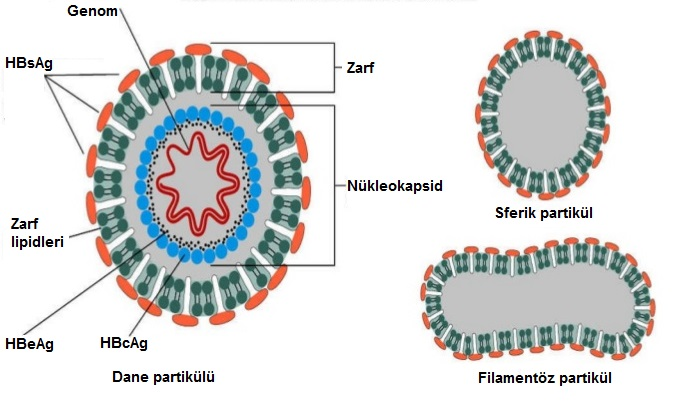
\includegraphics[width=0.6\linewidth]{../Figures/HBVstructure}
\caption[Hepatit B virüsünün yapısı]{Hepatit B virüsünün yapısı \par ({\scriptsize McGraw-Hill Companies Inc'den kaynak alınmıştır})}
\label{fig:HBVstructure}
\end{figure}

\subsection{Hepatit B Virüsü'nün Yapısı, Proteinleri ve Enzimleri}


\textbf{Virion}: DNA genomu, viral kapsid ve bunu saran zarfı içeren 42 mm çaplı enfeksiyoz küresel yapıdır (Dane partikülü).

\textbf{Zarf}: Lipoprotein yapıdadır ve nükleokapsidi çevreler. Membran lipidleri hepatosit membranı kökenlidir. Zarf yüzeyindeki HBsAg ise polipeptid yapıdadır. 

\textbf{Kapsid}: Viral genomu çevreleyen, protein yapılı HBV kapsidi ikozahedral (20 eşkenar üçgen yüz, 12 köşe) simetri göstermektedir. Hepatit B core antijen (HBcAg) ikişer ikişer disülfit bağları ile stabilize olduktan sonra bu birimlerden 180-240 tanesi bir araya gelerek kapsidi oluşturur. 

\textbf{Genom}: Kısmi çift sarmallı sirküler yapıda DNA içerir. Negatif iplikçik tam uzunluktadır, pozitif iplikçik ise kısmi tamamlanmıştır. 

\textbf{HBsAg (Hepatit B surface antijen)}: HBV'nin glikolize zarf proteinidir. Aktif covalently closed circular DNA (cccDNA)'dan ve integre DNA'dan sentezlenir. Büyük (L-HBsAg), orta (M-HBsAg), küçük (S-HBsAg) olmak üzere üç formu vardır (Şekil \ref{fig:hbsag}). S-HBsAg Dane partikülünde en fazla bulunan yüzey proteinidir. Fazla miktarda sentezlenerek hepatositten salınır. 

\begin{figure}[tbph]
\centering
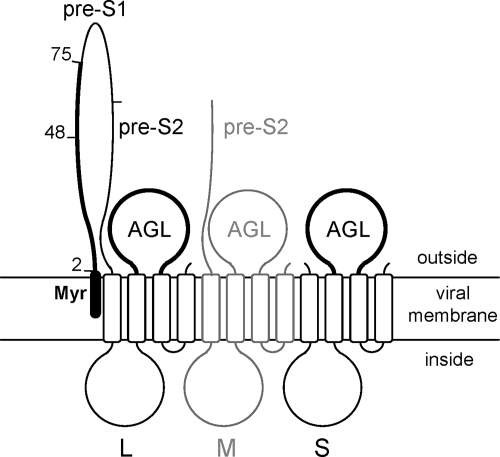
\includegraphics[width=0.45\linewidth]{../Figures/hbsag}
\caption[HBsAg'nin şematik görünümü]{HBsAg'nin şematik görünümü \cite{le2009pre} {\scriptsize \par AGL: Antigenic loop, Myr: Myristic acid}}
\label{fig:hbsag}
\end{figure}

\newpage

\textbf{HBcAg}: Viral DNA'yı çevreleyen kapsidin yapısı oluşturan proteinlerdir. Serumda serbest bulunmaz, hepatosit yüzeyinde eksprese edildiğinden immun yanıt oluşturur. 

\textbf{HBeAg (Hepatit B envelope antijen)}: Replikasyon için gerekli değildir, tam fonksiyonu bilinmemektedir. Hepatositten dışarı salınır. Viral DNA sentezlenmesinde kalıp olarak kullanılan pregenomik RNA (pgRNA)'dan sentezlendiğinde fazla saptanması, fazla miktarda pgRNA sentezlendiğini yani viral replikasyonun ve infektivitenin yüksek olduğunun göstergesidir. 

\textbf{HBV DNA polimeraz enzimi}: DNA polimeraz, revers transkriptaz ve RNase aktivitesi vardır. 

\textbf{HBx}: HBV replikasyonunda rol oynar, HBV'nin onkojenik potansiyaline katkıda bulunduğu bildirilmiştir \cite{liang2009hepatitis}.


\subsection{Hepatit B Virüsü'nün Genomu}

Genom, kısmi çift sarmallı sirküler yapıda ve yaklaşık 3,2 kb uzunluğundadır. Negatif iplikçik tamamlanmıştir, pozitif iplikçik ise değişen uzunluklardadır ve negatif iplikçikten daha kısadır. Negatif ipçiğin 5' ve 3' uçları arasında boşluk vardır ve negatif ipçik pozitif ipçik sayesinde halka şeklinde tutulur. Viral genomun bu yapısı gevşek sirküler DNA (rcDNA) olarak adlandırılır. Olgun virion içinde genom bu formdadır, replikasyon sırasında ise cccDNA; yeni oluşan kapsidlerin içinde ise polimeraz enzimi ile birlikte bulunan pgRNA formu halinde bulunur \cite{enfeksiyonlar3willke}.

HBV DNA üst üste binmiş 4 ORF (opening reading frame) içerir (Şekil \ref{fig:hbvgenom}):

\textbf{S (surface) geni}: Üç farklı zarf glikoproteini kodlar: Pre S1 (L-HBsAg), pre S2 (M-HBsAg) ve S proteini (S-HBsAg-Australia Antijen). 

\textbf{C (core) geni}: HBcAg ve HBeAg'yi kodlar.

\textbf{P (polimeraz) geni}: DNA polimerazı kodlar.

\textbf{X geni}: HBx'i kodlar. 


HBV'nin 10 genotipi (A-J) ve multipl subgenotipleri vardır. Farklı HBV izolatları \%90-\%98 aynı nükleotid sekansına sahiptir \cite{jawetz2013adelberg}. Ülkemizde baskın genotip Akdeniz ülkelerinde olduğu gibi genotip D'dir.

\bigskip

\begin{figure}[tbph]
\centering
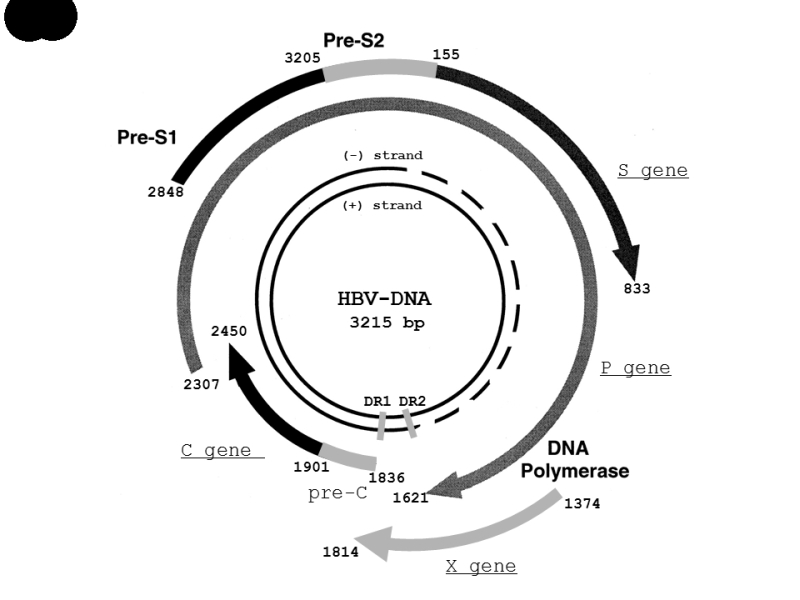
\includegraphics[width=0.7\linewidth]{../Figures/hbvgenom}
\caption[Hepatit B virüsünün genomu]{Hepatit B virüsünün genomu \cite{inoue2016hepatitis}}
\label{fig:hbvgenom}
\end{figure}

\subsection{Hepatit B Virüsü'nün Yaşam Döngüsü ve Hepatotropizm}


HBV'nin girişi; virionun hepatosit yüzeyinde bulunan hepatosit spesifik preS1 reseptörüne ve yüzey heparan sülfat proteoglikanlarına düşük afinite ile geri dönüşümlü olarak bağlanmasıyla başlar (Şekil \ref{fig:hbventry}). Virion; L zarf proteinin pre-S1 domaini ile NTCP (Na taurocholate cotransporting polypeptide)'ye bağlanır ve membran füzyonu ile sitoplazmaya kor partikülleri aktarılır \cite{yan2012sodium, watashi2014ntcp}. Hepatosit içine girişin endositoz ve füzyon ile olduğu öne sürülmüştür \cite{urban2010replication}. Viral DNA sitoplazmadan nükleusa girer ve rcDNA, cccDNA'ya dönüşür. cccDNA, konak polimeraz II'yi kullanarak negatif ipçikten viral transkripsiyonu başlatır. HBV'nin mRNA sentezini yöneten dört promoter bölgesi vardır: PreC/C, PreS1, S ve X promoter'leri (Şekil \ref{fig:hbvgenom}). Oluşan viral mRNA'lar sitoplazmaya gönderilir ve endoplazmik retikuluma bağlı ribozomlarda translasyon gerçekleşir. PreC/C bölgesi viral replikasyonun merkezidir ve pgRNA'yı sentezletir. pgRNA'dan HBcAg, HBeAg, polimeraz protenleri sentezlenir ve aynı zamanda pgRNA viral genom sentezi için kalıptır. Oluşan viral polimeraz pgRNA'nın enkapsidasyon dizisine bağlanarak viral kapsid yapımı başlatılır \cite{jeong2000evidence}. RNA'dan DNA sentezlenmesi anlamına gelen revers transkripsiyon yine polimeraz enzimi ile hücre sitoplazmasında viral kapsid içinde gerçekleşir. Negatif ipçik, sonrasında da pozitif ipçik böylece oluştuktan sonra sentezlenmiş HBsAg ile nükleokapsid birleşir, lipid zar kazanılarak hepatositten enfeksiyoz Dane partikülü olarak salınır ya da yeniden cccDNA oluşumu için nükleusa geri dönüştürülür \cite{yang2014persistence}.

Günde ortalama 10$ ^{11} $ yeni virionun meydana geldiği tahmin edilmektedir. Bu fazla ve hızlı virion üretiminin yanında DNA polimeraz enziminin proof reading fonksiyonunun olmaması replikasyon sırasında çok miktarda hata oluşmasında neden olmaktadır. 

\bigskip

\begin{figure}[tbph]
\centering
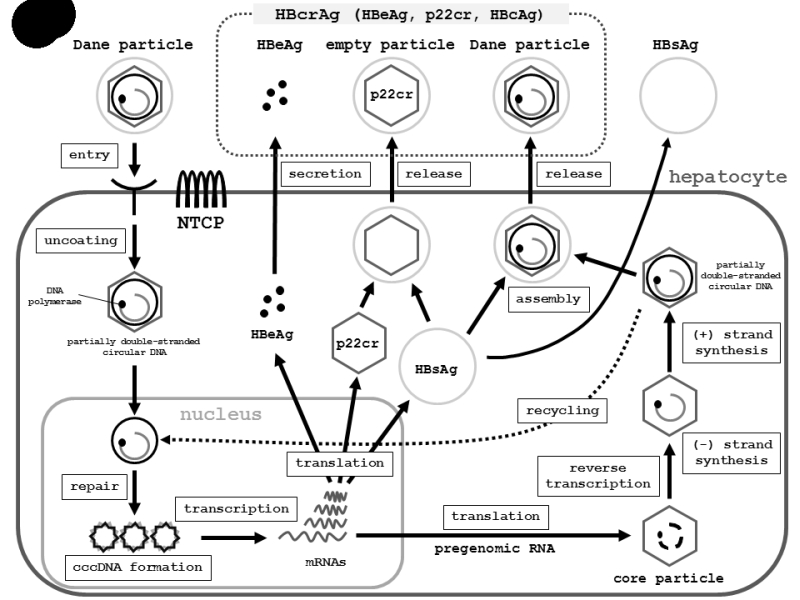
\includegraphics[width=0.9\linewidth]{../Figures/hbventry}
\caption[Hepatit B virüsünün hepatosite girişi, replikasyonu ve salınımı]{Hepatit B virüsünün hepatosite girişi, replikasyonu ve salınımı \cite{inoue2016hepatitis}}
\label{fig:hbventry}
\end{figure}


\subsection{Hepatit B Virüsü'ne Karşı İmmun Yanıt}

HBV’nin primer olarak replike olduğu yer hepatosittir. Direkt olarak sitopatik etkisi yoktur, virüse hücresel ve humoral immun yanıt oluşur. Humoral immun yanıt dolaşan virüs partiküllerini nötralize edip virüsün yayılımını engellemeye çalışırken, sellüler immun yanıt da enfekte hepatositleri öldürür \cite{chisari2010pathogenesis}. HBV, hücre yüzeyi ve endozomda Toll-like reseptörler ile, sitoplazmada da RIG-I (retinoic acid inducible gene I) ve MDA5 (melanoma differentiation gene 5) gibi sensörlerle immun sistem tarafından tanınır ve hepatosit, muhtemelen de diğer hücrelerden IFN salınır, aynı zamanda IFN ile stimule olan genler eksprese edilir \cite{sato2015rna,boeijen2017hepatitis}. Fakat HBV ile indüklenmiş bu IFN yanıtı zayıftır, hatta hayvan çalışmalarında HBV'nin IFN ekspresyonunu indüklemediği gösterilmiştir ve HBV'nin "gizlenen" bir virüs olduğu belirtilmiştir \cite{wieland2005stealth,wieland2004genomic}. Nukleusa cccDNA olarak adapte olmak da bu gizliliğe katkıda bulunur. Hangi patern tanıma reseptörlerinin ya da sinyal yolağının virüsün erken kontrolünde esas rolü oynadığı henüz bilinmemektedir.

Konak immun yanıtında karaciğer sinüzoidlerinde bulunan Kupffer hücreleri ve dendritik hücrelerin naif CD4+ ve CD8+ T hücrelerine antijen sunması da rol oynar ve yanıt aktivasyon ya da tolerans olarak gösterilir. 

Virüsle enfekte hepatositi tanıyan ve lizise uğratan naturel killer hücreler aynı zamanda IFN $ \gamma $ salgılayarak HBV'nin virüse spesifik CD8+ T hücreleri tarafından non sitolitik yolla temizlenmesini düzenler. Ayrıca cccDNA'nın integrasyonun engelleyen antiviral APOBEC ptoteinlerinin yapımı indüklenir.

Virüse spesifik CD4+ ve CD8+ T hücreleri, B hücreleri ve antikorlar HBV kontrolünde vazgeçilmezdir. HBV'ye karşı bu edinilmiş bağışıklık maruziyet sonrası 10 ila 12 haftada gelişir \cite{bertoletti2016adaptive,webster2000incubation}. Bu geç yanıtın virüsün gizli kalma doğasına katkıda bulunduğu düşünülmektedir ama kronikleşmede tek faktör bu değildir, virüsün kendiliğinden kontrol altına alındığı bireylerin çoğunda sonuçta bu gecikmiş yanıt gözlenmektedir.

Virüse spesifik CD4+ T lenfosit hücre yanıtı HBV kor epitoplarını, daha az olarak da yüzey antijeni, polimeraz ve x proteinini hedef alır. Akut, kontrol altına alınmış enfeksiyonlarda kronikleşmiş enfeksiyonlara göre daha hedefe yönelik ve güçlüdür. HBV'ye özgü CD8+ T hücre cevabı virüs temizlenmesinde ve KC hasar patogenezinde temel rolü oynamaktadır. Hepatositler tarafından viral antijenlerin CD8+ lenfositlere sunulmasıyla başlayan sitotoksik T hücre yanıtı enfekte hepatositi apoptoz ile öldürür, aynı zamanda IFN $ \gamma $ sekresyonunu uyarır. Akut hepatitte güçlüdür ve poliklonaldır kronik enfeksiyonda ise zayıftır. Zayıf sitotoksik T hücre yanıtı enfekte hepatositlerin temizlenmesinde yetersiz kalır ama yetersiz persistan hepatosit hasarı devam eder \cite{chisari2010pathogenesis}.


Erken çocuklukta virüse maruziyet ile oluşan kronik enfeksiyon, genellikle yüksek viremiye rağmen karaciğer hasarının bariz olmadığı immuntoleran faz ile karakterizedir. Bu fazda öne sürülen T hücre yanıtının ve/veya işlevinin olmadığıydı. Kronik HBV mekanizması ve immuntolerans sebebi net anlaşılamamakla birlikte sürekli antijen maruziyeti ile CD8+ T hücrelerinin fonksiyonlarının azalması/tükenmesi, inhibitör reseptörlerin ekspresyonu, sitokin proliferasyon kapasitesinin azalması,  viral yük, B ve T lenfosit inaktivasyona yol açan kaçış mutasyonları, viral antijenlerin kazanılmış immun cevabı baskılaması üzerinde durulmaktadır \cite{raziorrouh2010immunoregulatory,schurich2011role,chen2004function,webster2004longitudinal,reignat2002escaping}.



\section{HEPATİT B VİRÜS ENFEKSİYONU}

HBV; enfekte kişiden kan ve vücut sıvıları (semen, tükürük, servikal sekresyonlar, göz yaşı) ile penetran travma ya da mukozal temas ile bulaşabilmektedir. Yüksek prevelanslı bölgelerde HBV’nin enfekte anneden bebeğe perinatal geçişi en sık bulaş yoludur. Düşük prevelanslı bölgelerde ise çocuk doğurma çağındaki kadınlarda HBV enfeksiyon oranının az olmasıyla perinatal bulaş düşüktür ve bu bölgelerde bulaş genellikle adölesan ve yetişkin dönemde seksüel temas, iv ilaç kullanımı, enfekte kan ve kontamine aletlerle olmaktadır. 


HBV infeksiyonunun kliniği ve seyri virüs replikasyonu ve buna karşı immmun sistem yanıtı ile şekillenir. Virüse karşı kuvvetli immun yanıt ile akut-kendini sınırlayıcı hepatit; aşırı ve kontrolsüz yanıt ile fulminan hepatit kliniği oluşabilir. Yetersiz yanıt, tolerans ile virüsün temizlenememesi sonrası HBV kronikleşebilir. Perinatal dönemde HBV’ye karşı immun sistemin tolerans göstermesiyla akut hepatit B tablosundan ziyade kronikleşme görülmektedir böylece siroz ve HCC riski daha fazladır. Adölesan, yetişkin dönemde HBV infeksiyonunda enfeksiyonu akut kendini sınırlayan klinikle ortaya çıkmaktadır ve kronikleşme az; dolayısıyla siroz, HCC riski düşüktür (Şekil \ref{fig:akuthbv}) . 


\begin{figure}[tbph]
\centering
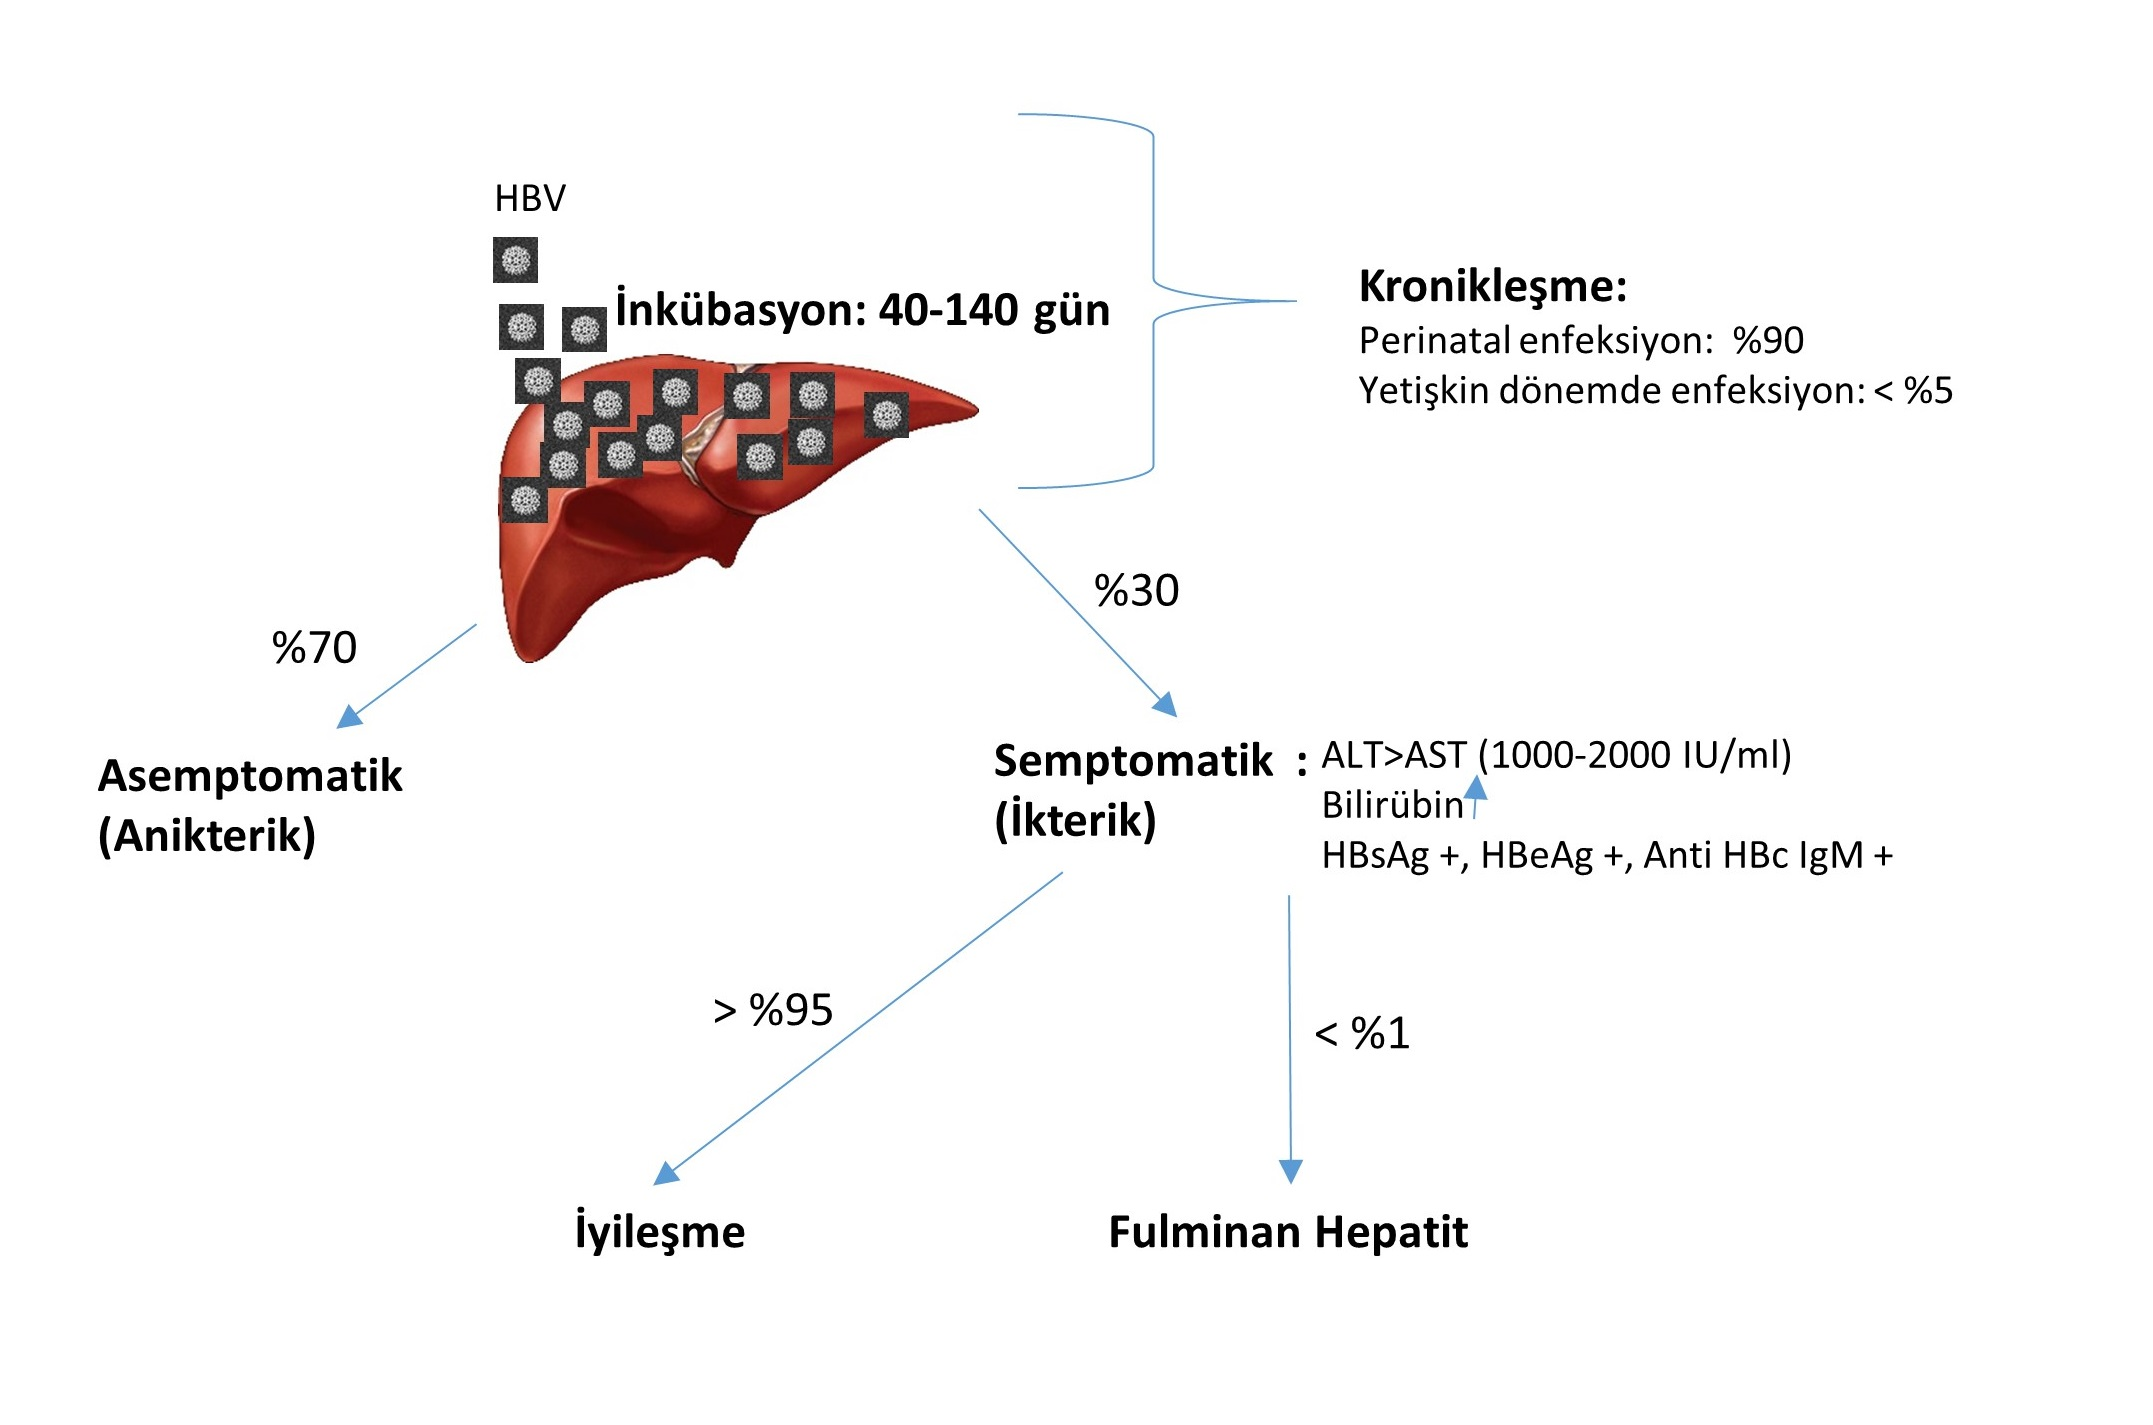
\includegraphics[width=0.8\linewidth]{../Figures/akuthbv}
\caption[Akut HBV enfeksiyonu]{Akut HBV enfeksiyonu \cite{terrault2016aasld}}
\label{fig:akuthbv}
\end{figure}



\subsection{Kronik Hepatit B}

HBsAg'nin 6 ayın üzerinde kanda pozitif saptanmasına kronik hepatit B (KHB) enfeksiyonu tanımlaması yapılmıştır. KHB'nin doğal seyri, HBV replikasyonu ve buna karşı immun yanıtımız çerçevesinde "kronik enfeksiyon" ve "hepatit" kavramları üzerinde yoğunlaşılarak beş faza ayrılmıştır \cite{european2017easl}. Fazların seyri karışıktır, sırayla olmayabilir, bir hastada her faz görülmeyebilir, fazlar arasındaki geçiş süreleri her hastada aynı değildir. Genelde erken yaşlarda enfekte olan kişilerde geçerlidir. 

\textbf{HBeAg pozitif kronik HBV enfeksiyonu (İmmuntoleran Faz):} Esas olarak doğum sırasında ya da erken çocukluk dönemde, nadiren de sonraki yıllarda bulaş ile ortaya çıkmaktadır. Konağın immuntoleransı sebebiyle HBV olabildiğince replike olmakta fakat immun yanıt gelişmediğinden KC'de nekroinflamasyon ve fibrozis oluşmamaktadır. HBeAg pozitif, HBV DNA yüksek, ALT normaldir. KC biyopsisinde inflamasyon/fibroz yoktur ya da minimaldir. Bulaştırıcılık yüksektir. Bu fazın süresi değişkendir, virüsün perinatal kazanımında en uzundur. Yüksek düzeyde HBV DNA integrasyonu olduğundan karsinogenez başlamış olabilir \cite{mason2016hbv}.

\textbf{HBeAg pozitif kronik hepatit B (İmmun Reaktif Faz):} İmmun sistemin reaksiyon göstermeye başlamasıyla hepatosit nekroinflamasyonu başlamıştır. HBeAg pozitiftir, HBV DNA immuntoleran faza göre azalmış olmakla birlikte yüksektir. ALT, immun yanıt ile hepatosit lizisi olduğundan yüksektir. KC'de orta-yüksek nekroinflamatuar aktivite vardır. Fibroza gidiş hızlanmıştır. İmmuntoleran fazdan bu faza geçişin 20'li ya da 30'lu yaşlarda olması beklenmektedir.  Çoğu hasta HBe serokonversiyonu ve HBV DNA baskılanmasıyla HBe negatif kronik HBV enfeksiyonu fazına geçer.

\textbf{HBeAg negatif kronik HBV enfeksiyonu (İnaktif taşıyıcılık):} HBeAg negatif, Anti-HBe pozitif, serum HBV DNA saptanamaz ya da düşük düzeyde, sürekli normal ALT düzeylerinde karaciğer histopatolojisinde hasar yok ya da minimaldir.

\textbf{HBeAg negatif kronik hepatit B: } Anti-HBe oluşmuştur, HBV DNA ve ALT yüksektir. Dalgalı seyir görülebilir, hepatik inflamasyon devam etmektedir. Çoğu vakada kor/prekor mutasyonu sebebiyle HBeAg eksprese edilememektedir.

\textbf{HBsAg negatif faz:} HBsAg negatif, Anti-HBe negatif ya da pozitiftir. ALT genelde normal, HBV DNA saptanamaz düzeydedir. HBsAg seroklirensi sirozdan önce olduysa siroz, HCC riski düşüktür. İmmunsupresyon ile reaktivasyon riski bu hasta grubunda mevcuttur.  


KHB'de antiviral ilaçların kullanım amacı kronik zamanda siroz ve hepatoselüler karsinoma ilerleyişi yavaşlatmak ve bunlara bağlı ölümü engellemektir. Akut hepatit durumunda antiviral tedavinin fulminan hepatite gidişi önleyip önlemediği tartışmalıdır. Şu an elimizdeki antiviral ilaçlar HBV replikasyonunu baskılayabilmektadır; HBV DNA'nın konak genomuna entegre olması, hepatosit nükleusu içindeki cccDNA'nın güncel antiviral ilaçlar ile inhibe edilememesi, HBV'ye karşı immuntolerans (örn. immuntoleran hastalar) gibi sebeplerle eradikasyon ya da kür sağlanamamaktadır  \cite{locarnini2015strategies}.


\subsection{HBeAg Negatif Kronik HBV Enfeksiyonu (İnaktif Taşıyıcılık)}

1987'de Hoofnagle ve arkadaşları HBsAg (+) hastaları kronik hepatit B ve asemptomatik veya sağlıklı taşıyıcı hastalar olarak iki gruba ayırmıştır \cite{hoofnagle1987chronic}. Yapılan çalışmalarda HBsAg (+) bireylerin çoğunda ALT düzeyinin normal olduğu görülmüş, fibrozu saptamak için her hastaya invaziv girişim yapmanın zor, anlamsız olması ve maliyet etkin olmaması HBV DNA için eşik değer arayışlarına yöneltmiştir. 2000'de National Institute of Health tarafından asemptomatik veya sağlıklı taşıyıcılık yerine inaktif HBsAg taşıyıcılığı terminolojisi kullanılmaya başlanmış ve 20000 IU/mL değeri aktif/inaktif hepatit için eşik değeri olarak belirlenmiştir \cite{lok2001management}. Fakat seri HBV DNA ölçümleri ile HBeAg negatif KHB hastalarının yanlış olarak inaktif taşıyıcı olarak değerlendirildiğine dair çalışmalar sonucu eşik değer 2000 IU/mL'ye indirilmiştir \cite{chu2002quantitative,cacciola2005virological}.


Günümüzde, ALT düzeyi normal, HBeAg negatif, Anti-HBe pozitif, HBV DNA saptanamaz ya da düşük seviyede (<2000 IU/ml) olan hastalar ile HBV DNA >2000 IU/mL olup  (genelde 20000 IU/ml'nin altında) ALT düzeyi devamlı normal, karaciğer biyopsisinde minimal nekroinflamatuar aktivite ve düşük fibroz olan hastalar bu fazda olarak değerlendirilir \cite{european2017easl,terrault2016aasld,sarin2016asian}. 


\subsection{HBeAg Negatif Kronik HBV Enfeksiyonunda Komplikasyonlar}

HBeAg negatif kronik HBV enfeksiyonunda antiviral ilaç endikasyonu yoktur. Doğru olarak tanı konduğunda uzun vadede prognoz iyidir, en çok görülecek senaryo yıllar boyu kronik KC hastalığı komplikasyonu olmadan takiptir. Yine de reaktivasyon, siroz ve HCC nadir ama mümkün komplikasyonlardır.    

\textbf{REAKTİVASYON:} Serum HBV DNA'nın yeniden yüksek değerlere ulaşması ve karaciğerdeki nekroinflamatuar aktivitenin artması ile bunun ALT yükselmesi olarak laboratuvara yansımasıdır. HBeAg yeniden pozitifleşebilir. Alevlenmelerle KC'de fibroz düzeyi artabilir. HBV reaktivasyonu kendiliğinden ya da immunsupresif tedavi ile olabilir. HAV, HCV, HDV, HEV ile süperenfeksiyon ve diğer viral hepatit dışı sebepler (ilaç, alkol vb) akılda tutulmalıdır. Kemoterapötik ajanlar (öz. rituksimab ve antrasiklin grubu), kortikosteroidler, metotreksat ve anti-TNF$ \alpha $ kullanımı ile reaktivasyon ve hepatik dekompansasyon riski vardır \cite{yeo2006diagnosis,yeo2008hepatitis,xuan2014hepatitis}. ALT'deki 2 kat artış ile birlikte HBV DNA'nın >20000 IU/ml'nin sonuçlandğı veya saptanabilir HBV DNA düzeyinin reaktivasyon olarak kabul edildiği çeşitli çalışmalarda insidans 0.4 ile 4.7 arasındadır \cite{martinot2002serum,papatheodoridis2008longitudinal,chu2007spontaneous,kumar2009spontaneous,tong2013hepatitis,zacharakis2008role}.


\textbf{FİBROZ/SİROZ:} Yıllarca süren kronik immun yanıt ile hepatosit destruksiyonu ve rejenerasyon siklusları fibroz, siroz ve HCC'ye sebep olur. İnaktif taşıyıcılık tanımında KC'de nekroinflamatuar aktivitenin olmadığı ya da minimal olduğu kabul edilmiştir. Böylelikle bu fazda olduğu kabul edilmiş hastalara KC biyopsisi önerilmez. Fakat yapılan çeşitli çalışmalarda ALT ve DNA düzeyine göre inaktif kabul edilmiş hastaların \%10'unda KC hasarının atlanabileceği görülmüştür \cite{villa2011natural,papatheodoridis2012follow}. Bu hasar doğal klinik seyirdeki HBeAg (+) KHB fazında oluşmuş olabilir. 


\textbf{HEPATOSELÜLER KARSİNOM:} HCC tüm dünyada en sık görülen kanserlerde altıncı sırada olup kanser ile ilişkili mortalitenin üçüncü sebebidir. Etyoloji coğrafi farklılık göstermektedir. Uzakdoğu ve sahra altı Afrika'da daha erken yaşta gelişir ve genetik faktörler, HBV ve ek karsinogenler ile ilişkilidir, batıda ise genellikle geç yaşlarda ve siroz zemininde gelişir. Doubling time 4-6 aydır.   Taraması biyokimyasal ve radyolojik tetkiklerle yapılmaktadır, tanısı ise MR'daki tipik görüntü paterniyle ve/veya biyopsi ile konur. Biyokimyasal testlerden genelde AFP çalışılmıştır. Dünyadaki HCC vakalarının \%50-55'i, endemik bölgelerdeki HCC vakaların ise \%70-80'i HBV'ye atfolunur. Siroz, HCC için öncü kliniktir fakat KHB hastalarının yılda yaklaşık \%0.1'inde siroz olmadan da HCC gelişebilir \cite{fattovich2008natural,chayanupatkul2017hepatocellular}. HCC oluşumunda çok sayıda HBV'ye ve hastaya bağlı faktör rol oynar. Konak genomuna entegre olmuş HBV DNA ve mikrodelesyonlar hücresel bölünme kontrol mekanizmalarını bozarak onkogen etkisi gösterebilir \cite{matsubara1990integration}. Buna ek olarak bazı HBV proteinleri direkt olarak HCC gelişiminde rol oynayabilir. HHBx'in çeşitli transkripsiyon faktörleri, tümor supresyon genleri ve DNA tamirinde rol alan proteinlerle  etkileşimde bulunduğu gösterilmiştir \cite{chisari2010pathogenesis,kremsdorf2006hepatitis}.

İnaktif taşıyıcılarda HBV DNA saptanamaz düzeyde olsa bile, HBV ile enfekte olmayan populasyona göre HCC riski daha fazladır \cite{chen2010carriers}. İleri yaş, ailede HCC öyküsü, siroz varlığı, alkol kullanımı, HBV DNA yüksekliği, ALT yüksekliği, HBe serokonversiyon süresinin uzaması HCC gelişimi için risk faktörleridir. HBsAg serokonversiyonu sonrası da HCC riski devam etmektedir bu sebeple özellikle serokonversiyon gelişmiş 50 yaş üstü erkek hastalarda HCC taramasının devam etmesi önerilmektedir \cite{yip2017impact}. Diğer HCC taramasının önerildiği KHB taşıyıcı hasta grupları sirotik hastalar, 50 yaş üstü Asya kökenli kadınlar, 40 yaş üstü Asya kökenli erkekler, ailede HCC öyküsü olanlar, Afrikalı-Kuzey Amerikalı siyahiler ve sirozlulardır \cite{bruix2011management}. HCC oranlarının yüksek belirtildiği yayınlar genelde Asya kaynaklıdır (Öz. Tayvan). Bunun nedeni perinatal dönemde kazanılmış HBV, genetik faktörler ve ek karsinojenler olabilir. Düşük düzey DNA ve normal ALT ile uzun süre takip edilen taşıyıcıları içeren Avrupa kaynaklı yayınlarda bu oran daha düşüktür. 

Özellikle riskli gruptaki hastalarda görüntüleme yöntemleri ile tanıda geç kalmamak adına HCC taraması devam etmelidir. Semptomlar çıktığından sonra saptanmış HCC'de 5 yıllık prognoz kötüdür.




\textbf{HBsAg SEROKLİRENSİ:} KHB'de immun kontrolün sağlandığının en iyi serolojik göstergesidir. HBsAg seroklirensi ve Anti-HBs serokonversiyonu genellikle birkaç yıl saptanamaz düzeyde seyreden HBV DNA ölçümlerinden sonra yılda \%1-\%3 hastada görülmektedir \cite{martinot2002serum}.  Seroklirens genç yaşta, fibroz gelişmeden oluştuğunda prognoz mükemmeldir ancak seroklirens esnasında sirozlu hastada klinik kötüye gidiş, dekompansasyon, HCC ve bunlara bağlı ölüm üzerinde etkisi yoktur.   

Tablo \ref{tablo:lit}'de literatürde inaktif taşıcılarda doğal seyir ile ilgili yaplmış çalşmalar gösterilmiştir


%\begin{\begin{landscape}
\begin{sidewaystable}
\begin{minipage}[c]{\textwidth}
\renewcommand{\arraystretch}{1.3} %SATIR ARALI^GI BEL'IRLEMEK 'IÇ'IN SAYIYI DE^G'I¸ST'IR'IN
\centering
\begin{threeparttable}
\caption[HBeAg negatif kronik HBV enfeksiyonunda doğal seyir ile ilgili literatüler]{HBeAg negatif kronik HBV enfeksiyonunda doğal seyir ile ilgili literatürler} \label{tablo:lit} %Tablo ba¸slı^gı ve referans etiketi
%---------------------------------------
{\scriptsize \begin{tabular}{llllL{1cm}L{1.4cm}L{1.4cm}llL{1cm}L{1.7cm}L{1.7cm}}
\toprule\toprule
                         & \textbf{ÜLKE} & \textbf{DİZAYN} & \textbf{N} & \textbf{İZLEM (YIL)} & \textbf{REAKT. N (\%)} & \textbf{REAKT. İNS} & \textbf{S N (\%)} & \textbf{HCC N (\%)} & \textbf{HCC İNS.} & \textbf{HBsAg KLR N (\%)} & \textbf{HBsAg KLR İNS. 100 kişi-yıl} \\
\midrule
Martinot-Peignoux (2002) \cite{martinot2002serum} \tnote{1,  } \:\tnote{a} & Fransa        & Prospektif      & 38         & 3.2                & 1 (1)                  & 0.8                      & 0                & 0                  &                        &                           &                              \\
Martinot-Peignoux (2013) \cite{martinot2013prediction} \tnote{1} \:\tnote{a} & Fransa        & Prospektif      & 54         & 10                 & 0 (0)                  &                          &                  &                    &                        & 8 (15)                    & 1.5           \\
Chen (2010) \cite{chen2010carriers} \tnote{1}            & Tayvan        & Prospektif      & 1932       & 13.1               &                        &                          &                  & 16 (0.82)          & 0.06                   &                           &                              \\
Habersetzer (2015) \cite{habersetzer2015loss}  \tnote{1}    & Fransa        & Prospektif      & 109        & 6                  &                        &                          &                  &                    &                        & 11 (3.5)                  & 2.3         \\
Magalhães (2015) \cite{magalhaes2015hepatitis} \tnote{1} \:\tnote{h}       & Portekiz      & Retrospektif    & 100        & 4.6                & 10 (10)                &                          & 0                & 0                  &                        & 4 (4)                     &                              \\
Tong ve Trieu (2013) \cite{tong2013hepatitis} \tnote{1} \:\tnote{f}    & USA           & Prospektif      & 146        & 8                  & 1 (0.7)                &                          & 0                & 2 (1.3)            & 0.17                   & 13 (9)                    & 1.1            \\
Papatheodoridis (2008) \cite{papatheodoridis2008longitudinal} \tnote{2} \:\tnote{e}   & Yunanistan    & Prospektif      & 85         & 3                  & 12 (14)                & 4.7                      &                  &                    &                        &                           &                              \\
Oliveri (2017)  \cite{oliveri2017long}   \tnote{2} \:\tnote{g}      & İtalya        & Prospektif      & 133        & 4.7                & 1 (0.75)               &                          & 0                & 0                  &                        & 21 (15.7)                 &                              \\
Gigi (2007) \cite{gigi2007long}    \tnote{2} \:\tnote{d}          & Yunanistan    & Retrospektif    & 307        & 7.4                & 73 (23.8)              &                          & 1                & 0                  &                        & 24 (7.8)                  &                              \\
Zacharakis (2008) \cite{zacharakis2008role} \tnote{3} \:\tnote{c}      & Yunanistan    & Prospektif      & 195        & 5.3                & 4 (2.1)                & 0.4                      & 0                & 0                  &                        & 16 (8.2)                  &                              \\
Chu ve Liaw (2007) \cite{chu2007spontaneous}  \tnote{3} \:\tnote{b}     & Tayvan        & Prospektif      & 1241       & 12.3               & 211 (17)               & 1.4                      & 40 (3.2)         & 4 (0.32)         &                        &                           &                              \\
Chu ve Liaw (2007) \cite{chu2007hbsag}  \tnote{3} \:\tnote{b}     & Tayvan        & Prospektif      & 1965       & 10.8               & 314 (15.9)             & 1.55                     &                  &                    &                        & 245 (12)                  & 1.2           \\
Kumar (2009)  \cite{kumar2009spontaneous}   \tnote{3} \:\tnote{a}        & Hindistan     & Prospektif      & 217        & 6.3                & 43 (19.8)              & 3.1                      &                  &                    &                        &                           &                              \\
Hsu (2002)  \cite{hsu2002long}   \tnote{3}          & Tayvan        & Prospektif      & 189        & 8.2                &                        &                          & 1 (0.5)        & 3 (1.6)            &                        & 9 (4.8)                   &                              \\
Taida (2016)  \cite{taida2017prognosis}   \tnote{4}        & Japonya       & Prospektif      & 388        & 2.8                &                        &                          & 0                & 0                  &                        &                           &     \\
\bottomrule                        
\end{tabular}}
%------------------------------------------
\footnotesize
\begin{tablenotes}
\item \textbf{REAKT.}: Reaktivasyon; \textbf{İNS.}: İnsidans; \textbf{S}: Siroz; \textbf{KLR.}: Klirens \par
\textbf{İnaktif Taşıyıcılık Kriteri:} \par
\item [1] HBeAg (-), Anti-HBe (+); ALT N, HBV DNA<2000 IU/ml \par
\item [2] HBeAg (-), Anti-HBe (+), ALT: N, HBV DNA<20000 IU/ml \par
\item [3] HBeAg (-), Anti-HBe (+), ALT:N \par
\item [4] HBeAg (-), Anti-HBe (+), ALT<31 U/L; HBV DNA<4 log kopya/ml \par
\textbf{Reaktivasyon Kriteri:} \par
\item[a] ALT$ \geq $ 2ULN ve/veya HBV DNA>20000 IU/ml \par
\item[b] ALT$ \geq $ 2ULN ve HBV DNA'nın saptanabilir düzeyde olması \par
\item [c] ALT yüksek ve HBV DNA >2000 IU/ml \par
\item [d] ALT yüksek ve HBV DNA >20000 IU/ml \par
\item [e] ALT artışı, saptanabilir HBV DNA ve KHB ile uyumlu histopatoloji \par
\item [f] ALT > 80 U/L ve HBV DNA   $ \geq $ 1000000 kopya/mL \par
\item [g] ALT N ya da yüksek ve HBV DNA >20.000 IU/ml \par
\item [h] Belirtilmemiş


%\item [$\S$] third note ;
%\item [**] the first note;
\end{tablenotes}
\end{threeparttable}
\end{minipage}
\end{sidewaystable}
%\end{landscape}}


\newpage

\subsection{HBeAg Negatif Kronik HBV Enfeksiyonu'nun Takibi}

İlk defa başvurmuş HBsAg pozitif bir hastadan ayrıntılı anamnez alınmalıdır. Bulaş yolu açısından annede ve diğer birinci derece akrabalarda HBsAg pozitifliğinin bilinip bilinmediği, riskli cinsel temas, diyaliz öyküsü, kan ve kan ürünleri nakli, ameliyat öyküsü, diş tedavisi, iv ilaç kullanımı sorgulanmalıdır. Komorbiditeler (obezite, diyabet, metabolik sendrom) değerlendirilmeli, kronik KC hastalığı açısından fizik muayenesi (ödem, ikter, batın kollateralleri, asit muayenesi vb) yapılmalıdır. HBV replikasyonu ve kronik KC hastalığı varlığı açısından hemogram, ALT, AST, ALP, GGT, total ve direkt bilirübin, albumin, protrombin zamanı, HBeAg, Anti-HBe, HBV DNA testleri ile koinfeksiyonlar için Anti-HCV, Anti-HDV, Anti-HIV; hepatit A virüsüne bağışıklığı belirlemek için de Anti-HAV IgG bakılmalıdır. Anti-HAV IgG negatif olanlar aşılanmalıdır. Birinci derece akrabalar ve partnerler de HBV için taranmalı, bağışıklıkları yoksa aşılanmalıdır. 


HBV DNA <2000 IU/ml, HBeAg negatif, ALT düzeyi normal olan bir hastada tek ölçüm ile inaktif taşıyıcılık tanısı konulmamalıdır. HBeAg negatif KHB'de HBV DNA ve ALT dalgalı seyredebileceğinden hastalar ilk yıl içerisinde üç ayda bir ALT ve periyodik olarak HBV DNA düzeyi takip edilmesi önerilmektedir \cite{european2017easl}. İnaktif taşıyıcılık ile HBeAg negatif KHB'nin ayrımı, iki kliniğin seyrindeki farklılık sebebiyle önemlidir. İnaktif taşıyıcılıkta prognoz iyidir, komplikasyonlara ilerleyiş riski düşüktür, HBeAg negatif KHB'de ise bu risk daha yüksektir. 


İlk bir yıllık takipte ALT düzeyi normal seyrediyorsa kontrol periyodu 6 aya çekilebilir. Yapılan çalışmalarda ilk ALT düzeyi normal olan hastaların ilk bir sene içinde yüksek bir ALT düzeyine sahip olma ihtimalinin \%15-20 olduğu görülmüş ve bu riskin 3 senelik takip sonrasında azaldığı gözlenmişir bu yüzden ilk 1-3 yılda yakın gözlem önemlidir \cite{papatheodoridis2012follow,papatheodoridis2008longitudinal}. 


Rehber önerilerine baktığımızda EASL 2017, HBV DNA < 2000 IU/ml olan hastalarda ALT'nin 6-12 ayda bir bakılmasını ve 2-3 yılda bir de KC fibroz durumunun değerlendirmesini; HBV DNA $ \geq $ 2000 IU/ml olan hastalardaysa en az 3 ayda bir ALT ve HBV DNA bakılmasını, her yıl da non invaziv bir test ile KC fibroz değerlendirmesinin yapılmasını önermektedir \cite{european2017easl}.

APASL 2015, HBV DNA < 2000 IU/ml olan hastalarda 3-6 ayda bir ALT ve AFP, 6-12 ayda bir de HBV ve KC USG takibini önermektedir. HBV $ \geq $ 2000 IU/mi ise de 3 ayda bir  HBV DNA ve ALT ile takip önermektedir \cite{sarin2016asian}. 

VHSD 2017 ise, inaktif taşıyıcıların 6-12 ayda bir HBV DNA, AFP ve KC USG ile takip edilmesini önermektedir \cite{vhsd2017}.  

Uzman görüşlerinde HBV DNA > 2000 IU/ml olan hastalara KC biyopsisi yapılabileceği belirtilmektedir. Çeşitli yayınlarda ALT düzeyi normal HBV DNA 2000-20000 IU/ml olan hastaların çok azında belirgin KC hasarı saptanmıştır. Bu hasta grubunda ALT ilk bir yıl 3 ayda bir, sonrasında 6 ayda bir HBV DNA ile değerlendirilmeli ve fibroz da non invaziv olarak senede bir kere üç sene boyunca takip edilmelidir. Üç sene sonrasında tedavi düşünülmüyorsa hayat boyunca diğer hastalar gibi takibe devam edilmelidir \cite{papatheodoridis2012follow}. Eğer ALT yükselir ve HBV DNA $ \geq $ 20000 olursa özellikle 35 yaş üstü ve ailesinde siroz/HCC öyküsü olan hastalarda karaciğerin invaziv ya da noninvaziv değerlendirmesi uygun olacaktır. 

\subsubsection{AFP, Görüntüleme Yöntemleri ve KC biyopsisi}

AFP, yolk kesesi ve fetal KC'den salgılanan bir plazma proteinidir. 8-12 yaştan itibaren yetişkindeki değerine düşer. Aynı endoderm kökenli organların tümörlerinde (HCC, mide kanseri, pankreas kanseri, intrahepatik kolanijokarsinomlar) serum AFP değerleri yükselebildiği gibi; tütün, alkol kullanımı, gebelik, kolon kanseri metastazları, testisin nonseminom germ hücreli tümörlerinde de yükselebilir. Karaciğerde kitle ve AFP yüksekliği direkt olarak HCC varlığını göstermez. HCC taramasında AFP'nin sensitivitesi ve spesifitesi yetersizdir \cite{bruix2011management}.


USG; kolay ulaşılabilirlik, radyasyon içermemesi ve düşük maliyetli olması gibi avantajlarla kronik KC hastalığı ve HCC taramasında kullanılır. Karaciğerin parenkim değerlendirmesi subjektiftir ve siroz tanısında duyarlılığu düşüktür. Birden fazla görüntüleme bulgusunun bir arada olması (parenkim ekosu yaygın kaba, karaciğer yüzeyinin nodüler görüntüsü, asit varlığı) daha kuvvetli olarak siroz düşündürür. HCC tanısında USG'un, BT ve MR'a göre duyarlılığı daha düşüktür ve rejeneratif nodüller, displastik nodüller ile küçük HCC odağı ayırt edilemeyebilir \cite{arif2014mri}.

USG'da 1 cm'den büyük nödül saptandığında 4 fazlı (erken arteryal, arteryal, venöz ve geç fazları içeren) dinamik BT ya da MR çekilmelidir. 1 cm'den küçük nodüllerde 3 ay sonra kontrol USG önerilmektedir, lezyonda büyüme yoksa USG takibi 3-6 ayda bir devam etmeli, boyut büyüdüyse 4 fazlı dinamik BT ya da MR çekilmelidir. HCC portal dolaşımdan kanlanmadığından arteryal hipervaskülarite ve venöz geç fazda kontrast kaybı (washout) görüntüsü HCC tanısı koydurur (Şekil \ref{fig:hcc}).  Bu tipik görüntü yoksa başka bir kontrastlı dinamik görüntüleme (BT ya da MR) çekilmelidir. Yine emin olunamıyorsa biyopsi yapılmalıdır \cite{bruix2011management}. 

\bigskip

\begin{figure}[tbph]
\centering
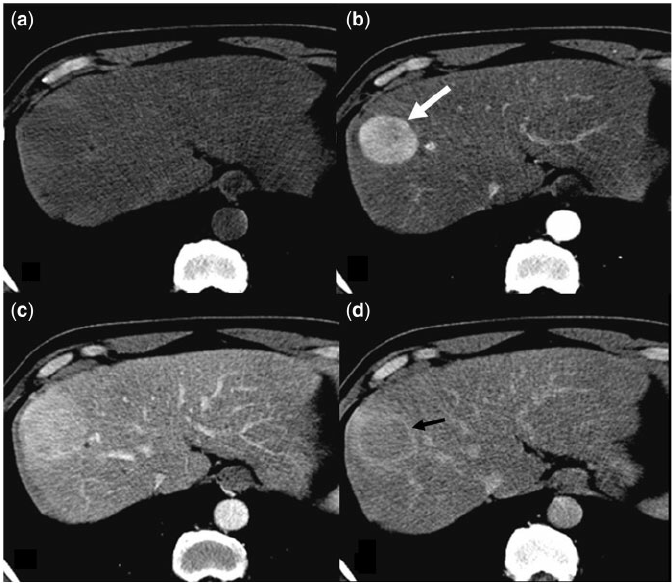
\includegraphics[width=0.7\linewidth]{../Figures/hcc}
\caption[Hepatoselüler karsinoma MR görüntüsü (washout patern)]{KHB'li bir hastada HCC'nin MR görüntüsü (washout patern) \cite{hennedige2012imaging} \par \textbf{(a)} Erken Faz-kontrast tutulumu yok \textbf{(b)} Arteriyel Faz, \textbf{(c)} Portal venöz faz, \par \textbf{(d)} Geç faz. İnce psödokapsül geç fazda görülmekte}
\label{fig:hcc}
\end{figure}


Kontrastlı dinamik MR ile anlatıldığı gibi biyopsi ihtiyacı olmadan tipik görüntü ile HCC tanısı konabilmektedir. >2 cm tümörlerde sensitivite artmaktedır. KC'in en fazla saptanan lezyonu hemanjiom ile ayrımın yapılmasında en iyi görüntüleme yöntemidir. 

Biyopsi KHB'de tanıdan ziyade KC hasarının belirlenmesi ile evrelendirmede ve olası diğer hastalıkların ekartasyonunda kullanılır. Antiviral ilaçlara yanıt ve hastalığın ilerleyişi de kontrol biyopsiler ile değerlendirilebilir. KC biyopsisi, KC'in yaklaşık 1/50.000'ini gösterir. KC'de fibroz heterojenite gösterdiğinden KC dokusunun gerçek durumu atlanabilir, aynı zamanda patologlar arasında değerlendirme farklılığı da bulunabilir. Biyopsi sonrası komplikasyonların yarısından fazlası ilk 2 saatte, neredeyse tamamı ilk 24 saat içinde olmaktadır. Bunlar sıklıkla ağrı, kanama, vazovagal refleks veya kanama ile açıklanabilecek hipotansiyon, yanlış anatomik bölgeye girilmesi sebebiyle oluşabilecek pnömotoraks, hemotoraks, safra kesesi perforasyonu, hemobili, pnömoperitoneumdur. Nondiagnostik biyopsi de bir diğer sorundur. Alınan parça en az 11 portal alan içermelidir bu da 16 gauge iğne kullanılarak alınmış en az 2 cm uzunluğundaki biyopsi materyali ile mümkün olur \cite{standish2006appraisal}. 

Biyopside patoloji tarafından KC'de nekroinflamasyon (Grade - Derecelendirme - Histolojik Aktivite İndeksi) ve fibroz (Stage - Evreleme) skoru verilir (Tablo \ref{tablo:ishakhai}), (Tablo \ref{tablo:ishakfib}). Bu skor ile takip ve tedavi yaklaşımı belirlenir. Histolojik aktivite indeksi KC'deki inflamasyon ve hepatoselüler hasarın göstergesi olup bu hasarın fibroza ilerleyebileceğini düşündürür. Evre ise fibrozun varlığını ve yaygınlığını gösterir \cite{guido2011chronic}.  

\bigskip

\begin{figure}[tbph]
\centering
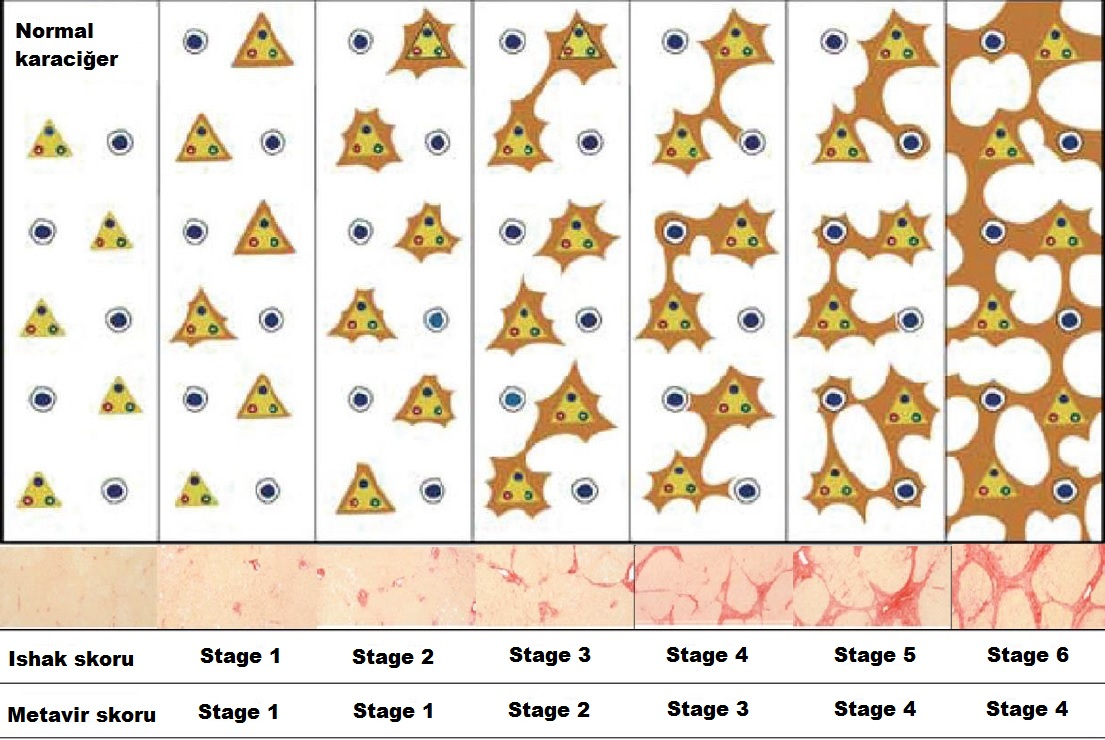
\includegraphics[width=0.9\linewidth]{../Figures/pato}
\caption[Ishak ve Metovir fibroz evrelemesi]{Ishak ve Metovir Fibroz Evrelemesi \cite{guido2011chronic,standish2006appraisal}}
\label{fig:pato}
\end{figure}






%\begin{\begin{landscape}
\begin{minipage}[c]{\textwidth}
\renewcommand{\arraystretch}{1.1} %SATIR ARALI^GI BEL'IRLEMEK 'IÇ'IN SAYIYI DE^G'I¸ST'IR'IN
\centering
\begin{threeparttable}
\caption[ISHAK skorlama sistemine göre modifiye
histolojik aktivite indeksi derecelendirmesi]{ISHAK skorlama sistemine göre modifiye
histolojik aktivite indeksi derecelendirmesi} \label{tablo:ishakhai} %Tablo ba¸slı^gı ve referans etiketi
%---------------------------------------
{\scriptsize \begin{tabular}{ll}
\toprule\toprule
\textbf{A. Periportal veya periseptal interface hepatiti (*piecemeal*)}              &   \\
\midrule
Yok                                                                                  & 0 \\
Hafif (fokal, birkaç portal alanda)                                                  & 1 \\
Hafif/Orta ( fokal, portal alanların çoğunda)                                        & 2 \\
Orta (trakt ya da septaların \%50’den azında, çevresinde devamlılık gösteren)        & 3 \\
Şiddetli (trakt ya da septaların \%50’den fazlasında, çevresindedevamlılık gösteren) & 4 \\
\midrule
\textbf{B. Konfluent nekroz}                                                         &   \\
\midrule
Yok                                                                                  & 0 \\
Fokal konfluent nekroz                                                               & 1 \\
Zon 3 nekroz (bazı alanlarda)                                                        & 2 \\
Zon 3 nekroz (çoğu alanda)                                                           & 3 \\
Zon 3 nekroz + seyrek portal-santral (P-C) köprüleşme                                & 4 \\
Zon 3 nekroz + çok sayıda portal-santral (P-C) köprüleşme                            & 5 \\
Panasiner veya mültiasiner nekroz                                                    & 6 \\
\midrule
\textbf{C. Fokal (*spotty*) litik nekroz, apoptozis fokal inflamasyon}               &   \\
\midrule
Yok                                                                                  & 0 \\
1 veya daha az odak (x 100’lik her büyütmede)                                        & 1 \\
2-4 odak (x 100’lük her büyütmede)                                                   & 2 \\
5-10 odak (x100’lük her büyütmede)                                                   & 3 \\
10’dan fazla odak (x100’lük her büyütmede)                                           & 4 \\
\midrule
\textbf{D. Portal inflamasyon}                                                       &   \\
\midrule
Yok                                                                                  & 0 \\
Hafif (bazı veya tüm portal alanlarda)                                               & 1 \\
Orta (bazı veya tüm portal alanlarda)                                                & 2 \\
Orta/Belirgin (tüm portal alanlarda)                                                 & 3 \\
Belirgin (tüm portal alanlarda)                                                      & 4 \\
\bottomrule
\end{tabular}}
%------------------------------------------
\begin{tablenotes}
%\footnotesize
%\item [*] Bazı hastalarda 2000-20000 IU/ml aralığında olup, ALT normal, KC hasarı yok/minimaldir.
%\item [**] Dalgalı seyir
%\item [$\dag$] second note ; %tabloya "\tnote{*}" ekleyin
%\item [$\ddag$] third note ;
%\item [$\S$] third note ;
%\item [**] the first note;
\end{tablenotes}
\end{threeparttable}
\end{minipage}
%\end{landscape}}



\bigskip

%\begin{\begin{landscape}
\begin{minipage}[c]{\textwidth}
\renewcommand{\arraystretch}{1.1} %SATIR ARALI^GI BEL'IRLEMEK 'IÇ'IN SAYIYI DE^G'I¸ST'IR'IN
\centering
\begin{threeparttable}
\caption[ISHAK skorlama sistemine göre fibrozis evrelemesi]{ISHAK skorlama sistemine göre fibrozis evrelemesi} \label{tablo:ishakfib} %Tablo ba¸slı^gı ve referans etiketi
%---------------------------------------
{\scriptsize \begin{tabular}{ll}
\toprule\toprule
\textbf{}                                                                                                        & \textbf{Skor} \\
\midrule
Fibrozis yok                                                                                                     & 0             \\
Birkaç portal alanda fibröz genişleme ve +/- kısa fibröz septa                                                   & 1             \\
Portal alanların çoğunda fibröz genişleme ve +/- kısa fibröz septa                                               & 2             \\
Portal alanların çoğunda fibröz ve seyrek portal –portal (P-P) köprüleşme                                        & 3             \\
Portal alanlarda fibröz genişleme ve belirgin köprüleşme{[}Portal-portal (P-P) yanı sıra portal-santral (P-C){]} & 4             \\
Belirgin köprüleşme (P-P ve/veya P-C) ile seyrek nodül (inkomplet siroz)                                         & 5             \\
Siroz (olası veya kesin)                                                                                         & 6      \\
\bottomrule    
\end{tabular}}
%------------------------------------------
\begin{tablenotes}
%\footnotesize
%\item [*] Bazı hastalarda 2000-20000 IU/ml aralığında olup, ALT normal, KC hasarı yok/minimaldir.
%\item [**] Dalgalı seyir
%\item [$\dag$] second note ; %tabloya "\tnote{*}" ekleyin
%\item [$\ddag$] third note ;
%\item [$\S$] third note ;
%\item [**] the first note;
\end{tablenotes}
\end{threeparttable}
\end{minipage}
%\end{landscape}}
     

Yukarıda belirtilen dezavantajlar sebebiyle biyopsiye olan ihtiyacı azaltmak ve biyopsinin kontrendike olduğu hastalarda KC fibrozu değerlendirmesinde ultrasonografik ileri görüntüleme yöntemleri ön plana çıkmaktadır. Bunlar transient elastografi, akustik radyasyon kuvveti impulsu görüntülenmesi (ARFI), shear dalgası elastografisi (SWE)'dir. Temel prensip dokunun sertliğini tespit etmektir.

Transient elastografide KC'e düşük frekanslı ve amplitüdlü titreşimler gönderilir. Eğer KC dokusunun esnekliği azalmış, sertliği artmışsa dalganın yayılım hızı artar ve bu hız probdaki dedektör ile saptanıp kilopaskal (kPA) cinsinden ifade edilerek fibroz miktarı belirlenir. 1.5-2.5 ile 75 kPA aralığında sonuç bildirilerek F0'dan F4'e kadar fibroz rapor edilir. Kolay uygulanabilir olması, biyopsi ile karşılaştırıldığında yaklaşık 100 kat daha fazla karaciğer parankimini taraması, komplikasyonsuz olması ve uygulayan kişiler arasında farklılığın az olması yöntemin avantajlarını oluştururken, orta derece fibrozisi ayırt etmede sensitivite ve spesifitesinin tam bilinmemesi, asitli hastalarda ve obez hastalarda ölçüm kalitesini bozulması dezavantajlarını oluşturmaktadır. Gebelerde ve implantı olan hastalarda kullanılması önerilmez \cite{alahdab17transient}.


\subsubsection{Sağlıkta Uygulama Tebliği'ne göre KHB tedavisi}
Takip ve yapılan tetkikler sonrasında KHB tedavisi düşünülürse güncel SGK Sağlıkta Uygulama Tebliği şu şekildedir:

\begin{itemize}
\item İlk tedaviye başlamak için; HBV DNA seviyesi 10.000 kopya/ml (2.000 IU/ml) veya üzerinde olan erişkin hastalara, bu durumun belirtildiği rapor ve eki tetkik sonuçlarına (HBV DNA sonucu ve karaciğer biyopsi raporu) göre karaciğer biyopsisinde Histolojik Aktivite İndeksi (HAI) $ \geq $6 veya fibrozis $ \geq $2 olan hastaların tedavisine interferonlar veya pegile interferonlar veya oral antiviraller ile başlanabilir. 

\item Erişkin hastalarda interferonlar ve pegile interferonlar ALT değeri normalin üst sınırının 2 katını geçen, HBeAg negatif olan ve HBV DNA $ \leq $ 10$ ^{7} $ kopya/ml olan hastalar ile HBeAg pozitif olan ve HBV DNA $ \leq $ 10$ ^{9} $ olan hastalarda kullanılabilir. İnterferonlar ve pegile interferonlar kronik hepatit B hastalarında en fazla 48 hafta süreyle kullanılabilir. 

\item Oral antiviral tedaviye erişkinde günde 100 mg lamivudin veya 600 mg telbivudin veya 245 mg tenofovir veya 0,5 mg entekavir ile başlanır. 

\item Erişkin hastalar oral antiviral tedavi altındayken lamivudin veya telbivudin tedavisinin 24 üncü haftasında HBV DNA 50 IU/ml (300 kopya/ml) ve üzerinde olan hastalarda diğer antiviraller kullanılır. Ancak bu tedavilerin 24 üncü haftasında HBV DNA 50 IU/ml (300 kopya/ml) altında ise başka bir oral antiviral ajana geçilemez veya eklenemez. Oral antiviral tedavisi alan hastalarda negatif olan HBV DNA’nın pozitifleşmesi veya HBV DNA’nın 10 kat yükselmesi ile başka bir oral antiviral ajana geçilebilir veya almakta oldukları tedaviye ikinci bir oral antiviral eklenebilir. Tenofovir veya entekavir ile tedavi alan hastalarda birinci yılın sonunda halen “HBV DNA pozitif” olması durumunda bu iki antiviral arasında geçiş yapılabilir veya bu iki antiviral birlikte kullanılabilir. Oral antiviral tedavisi alan hastalarda gebelik durumunda oral antiviral değişiminde bu koşullar aranmaz. Kullanılan antivirale karşı yan etki gelişmesi halinde koşul aranmaksızın başka bir antivirale geçilebilir. Oral antiviral değişimi ya da tedaviye yeni oral antiviral eklenmesi için, düzenlenecek yeni veya mevcut raporda bu durum belirtilir. Adefovir tedavisinde koşul aranmaksızın tenofovir veya entekavire geçilebilir.

\item Her yenilenen raporda tek başına HBsAg pozitifliği veya HBsAg negatifliği ile birlikte Anti-HBs negatifliği raporda belirtilmelidir. Oral antiviral tedavi, HBsAg negatif hastalarda Anti-HBs pozitifleştikten sonra en fazla 12 ay daha sürdürülür. Antiviral tedavi almakta olan hastaların raporlarının yenilenmesinde, başlama kriterlerinin hastanın tedavisine başlandığı tarihteki mevzuata uygun olduğu yeni raporda belirtilir.   

\end{itemize}



\section{SAĞLIK EKONOMİSİ}

Sağlık ekonomisi, ekonomi kurallarının sağlık hizmetleri alanına uygulanmasıyla ortaya çıkmış bir bilim dalıdır. Sağlık sektörüne ayrılmış tüm kaynakların maksimum sağlık hizmeti üretmek amacıyla en etkin ve verimli şekilde nasıl kullanılacağını ve topluma nasıl bölüştürüleceğini araştırır.
 
Sağlık harcamaları sadece bir gider kalemi olarak hesap edilmemelidir. Sağlık harcamaları ile toplumdaki bireylerin yaşam süreleri ve kaliteleri etkilenmektedir bu yönüyle diğer kamusal harcamalardan ayrılır. Teorik olarak sağlık söz konusu olduğunda (Ölümün olduğu yerde daha ciddi ne olabilir?) alınan tıbbi eğitim ve tecrübeler eşliğinde akla gelebilecek her türlü tarama yaklaşımlarının uygulandığı, laboratuvar ve görüntüleme tekniklerinin kullanılabildiği bir toplum hayal edilir. Fakat gerçek dünyada kaynaklar kısıtlı olduğundan kamu parası kullanılırken sağlık hizmetlerinin kendi içinde önceliklendirmesine önem verilmelidir. Sağlık ekonomisinde amaç tüm kaynakların verimli ve etkin kullanılmasıdır. 

\subsection{Maliyet} 

\begin{enumerate}[1.]\itemsep-6pt
\item \textbf{Doğrudan (Direkt) maliyet:} Laboratuar testleri, poliklinik ücretleri, tanıya yönelik yapılan görüntüleme teknikleri ve girişimsel işlemler, ilaç ücretleri gibi hasta, kurum, kamu veya özel geri ödeme sistemi tarafından karşılanması gereken harcamalardır.
\item \textbf{Dolaylı (İndirekt) maliyet:} Hastalığın morbidite ve mortalitesi sonucu verimlilik kaybı, üretime katkısının sonlanması ile ortaya çıkacak ekonomik kayıplardır. Hastane yatışı esnasında hastanın iş gücüne katılamaması ile çalışılan gün kaybı veya hastalık sonucu sakat/sekelli kalıp daha uzun yaşama sonucu gelecekteki ek maliyetlerin ortaya çıkması örnek gösterilebilir.
\item \textbf{Soyut maliyetler:} Hastalığa bağlı ortaya çıkan etkilerle kişinin yaşam kalitesindeki kaybın ölçüldüğü soyut bir maliyettir. QALY (Quality Adjusted Life Year-Kaliteye Endeksli Yaşam Yılı) her bir ömür senesini yaşam kalitesiyle birlikte ele alan bir ölçüttür. QALY yönteminde hastalar kendi sağlıklılık değerlendirmelerini 0 ile 1 arasında puanlarlar. 1 QALY mükemmel yaşam kalitesiyle geçirilmiş bir yılı temsil ederken 0 QALY ölümü temsil eder. Tabii “ölümden beter” olarak değerlendirilen durumlar olduğunda bunlar negatif değerler ile belirtilirler. 
Yaşanan yıl (n) X kişinin kendi yaşam kalitesi değerlendirmesi (0 – 1 arası değer) = QALY olarak hesaplanır. 
QALY hesaplaması her hastalık için aynı derecede hassas değildir, yaşam kalitesini arttıran tedavilerin değerlendirmesinde tercih edilebilir.

QALY dışında sık kullanılan yaşam kalitesi ölçütlerinde EQ5D (European Quality 5 Dimension), SF36 (Short Form 36), SF12 (Short Form 12), McMaster Sağlık İndeksi Anketi (McMaster Health Index Questionnaire), Nottingham Sağlık Profili (Nothingham Health Profile), Hastalık Etki Ölçeği (Sickness Impact Profile), Dünya Sağlık Örgütü Yaşam Kalitesi Ölçeği (World Health Organization Quality of Life Quastionnaire, WHOQOL) sayılabilir. 
\end{enumerate}


\subsection{Kârlar/Sonuçlar}

\begin{enumerate}[1.]\itemsep-6pt
\item \textbf{Ekonomik kârlar:} Yapılan tüm tasarruflar para birimi olarak hesaplanır ve ekonomik kâr olarak değerlendirilir.
\begin{enumerate}[a.]\itemsep-6pt
\item \textbf{Doğrudan kârlar:} Tanı koyarken, hastayı izlerken yapılan tasarruflardır.  Fazladan laboratuvar ve görüntüleme yöntemlerinden tasarruf, hastanede yatış süresini kısaltma, uygun taramayla hastalığa erken safhada tanı konarak olası komplikasyonların engellenmesi ile medikal tedavi/cerrahi masrafların da engellenmesi, poliklinik kontrol başvurularının azaltılması vb...
\item \textbf{Dolaylı kârlar:} Hasta ya da hasta yakınının iş kaybının engellenmesi
\item \textbf{Tanımlanamayan kârlar:} Hastanın tedavi ile şikayetlerindeki gerilemenin dikkate alınmasıdır. Hesaplanması zor, subjektiftir.
\end{enumerate}
\item \textbf{Sağlıksal etkiler/kârlar:} Yapılan tedaviler sonucu etkilerin tıbbi birimlerle ifadesidir. Kan basıncındaki mmHg düşüş, semptom skorlarında değişiklikler (Alerjik rinit semptom skorlaması, prostat semptom skoru...) vb...
\end{enumerate}

\section{SAĞLIK HARCAMALARINA İLİŞKİN GÜNCEL BİLGİLER}

\subsection{Ülkemizdeki Genel Durum}

Türkiye İstatististik Kurumu’nun verilerine göre Türkiye’de sağlık harcamaları artmaktadır. 2016 yılında sağlık harcamaları \%14.5 artışla 119 milyar 756 milyon TL’ye ulaşmış, kişi başı sağlık harcaması 2015 senesinde 1345 TL iken 2016 senesinde \%13.3 artarak 1524 TL’ye yükselmiştir. Sağlık harcamalarının \%78.5'u genel devlet bütçesinden, \%16.3'ü hane halkları tarafından karşılanmıştır \cite{tuik2017}.

OECD (Ekonomik Kalkınma ve İşbirliği Örgütü)'nin 2017 sağlık istatistikleri raporuna göre Türkiye'de sağlık durumu ve harcamalar ile ilgili vurgu yapılan noktalardan birkaçı şu şekildedir \cite{oecd2017}

\begin{itemize}
\item Yaşam beklentisi OECD ortalamasının altındadır. Erkeklerde 75.3 yıl (OECD ülkeleri ortalaması: 77.9), kadınlarda ise 80.7 yıldır (OECD ülkeleri ortalaması: 83.1). Buna rağmen Türkiye 1970'den beri sağlıklı yaşam beklentisi kazanımı en fazla olan ülkeler arasındadır. Sebepleri arasında gelir artışı, eğitim, sağlık sigortasına katılımın artması sayılabilir. 
\item Nüfusun \%98.4'ünün sağlık sigortası vardır.
\item OECD ülkeleri arasında kişi başına düşen sağlık harcaması en düşük olan ülkeler arasındadır (Kişi başına 1088 Amerikan doları). Sağlık harcamaları tüm ülkelerde artma eğilimindedir.
\item Gayri safi yurt içi hasılada sağlık harcamalarına ayrılan pay \%4.3'tür. Bu oranda Hindistan ile birlikte son sıralardayız. 
\item Kişi başına düşen doktor ve hemşire sayısı en düşük ülkeler arasındadır (Sırasıyla 1.8/1000 kişi; 2/1000 kişi)
\item Kişi başına düşen yatak sayısı ülkemiz hariç genel OECD ülkelerinde azalma eğilimindedir.
\item İlginç bir şekilde Türkiye en çok MRI çekilen ülkedir (144.3/1000 kişi).
\end{itemize}

İlaç kullanımımıza baktığımızda pazarda toplam tutar ölçeğinde en çok paya sahip ilaç grubu onkolojik ilaçlar olmuştur, ikinci sırada antibiyotikler gelmektedir. Kutu ölçeğinde ise en çok tüketime sahip ilaç grubu ise 2010’dan beri azalma eğiliminde olmasına rağmen hala antibiotiklerdir \cite{sektor17}.



\begin{minipage}{0.49\textwidth}
 \begin{center}
 	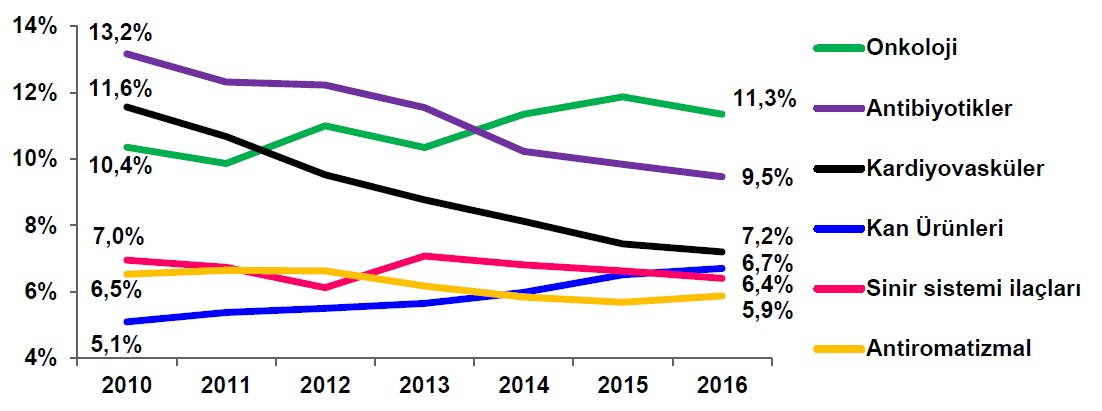
\includegraphics[width=1\linewidth, height=0.15\textheight]{../Figures/eko1}
 	\end{center}
 	  %\vspace{0pt}
 	  \captionof{figure}[İlaçların toplam tutar üzerinden payları]{İlaçların toplam tutar üzerinden payları \cite{sektor17}}
 	  \label{fig:eko1}	
\end{minipage}
\begin{minipage}{0.49\textwidth}
	\begin{center}
	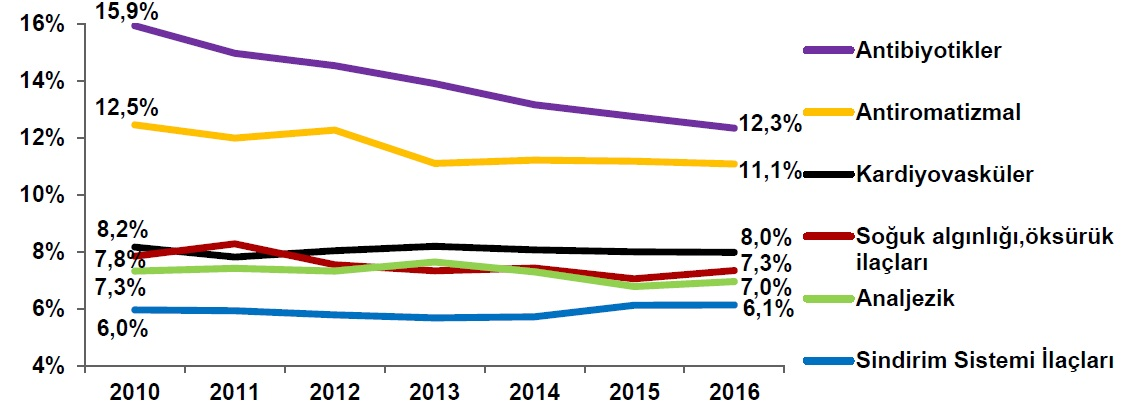
\includegraphics[width=1\linewidth, height=0.15\textheight]{../Figures/eko2}
	\end{center}
	  %\vspace{0pt}
	  \captionof{figure}[İlaçların kutu ölçeğinde payları]{İlaçların kutu ölçeğinde payları \cite{sektor17}}
	  \label{fig:eko2}
\end{minipage}\\



\subsection{Kronik Hepatit B'de Maliyet}

KHB'de en çok hasta yükünü taşıyıcı grup oluşturmaktadır fakat bu grup aynı zamanda KHB hastaları arasında en az harcama yapılan gruptur. Antiviral kullanımı ile ve komplikasyon oluştuğunda kişi başına düşen maliyet artmaktadır. Antiviral ilaç kullanımından fayda görecekleri tanımak komplikasyon gelişme riskini azaltacağından maliyet etkindir. 

Viral hepatit için ilk sırada istenen tarama testlerinin fiyatı 0.5-3 dolardır. Nükleik asit testleri ise 25-200 dolardır \cite{world2017global}. 

Antiviral ilaçlar kullanımıza baktığımızda IMS (Intercontinental Marketing Services) verilerine göre  2017 yılının ilk 6 ayında net kutu bazında satış rakamları şu şekildedir: Tenofovir disoproksil fumarat 290.412; entekavir: 124.912; lamivudin: 59.912; telbivudin: 14.606.  



\phantomsection
	
	%----------------------------------------------------------------
\newpage
\chapter{YÖNTEM} % Main chapter title
\label{MM} % For referencing the chapter elsewhere, use \ref{Chapter1} 
\lhead{\emph{Gereç \& Yöntemler}} % This is for the header on each page -
%perhaps a shortened title
%----------------------------------------------------------------------------------------
% Mate & Met
%---------------------------------------------------------------------- ------------------

\section {ÇALIŞMANIN TASARIMI} Bu retrospektif çalışma Istanbul Medeniyet Üniversitesi Göztepe Eğitim ve Araştırma Hastanesi Enfeksiyon Hastalıkları polikliniğine başvuran hastaların verileri elektronik ortamda taranarak yapıldı. 01.06.2016 - 01.06.2017 tarihleri arasında polikliniğimize başvurmuş hastaların kayıtlı tanıları incelendi. ICD-10 tanı kodları listesinden Z22.5 Viral hepatit taşıyıcısı; B18.0 Kronik viral hepatit B, delta ajansız, K74 Karaciğer fibroz ve sirozu; C22.0 Hepatoselüler karsinom tanıları ile Z13.9 Tarama muayenesi, tanımlanmamış; Z24.6 Viral hepatite karşı bağışıklama ihtiyacı; Z20.5 Viral hepatite temas ve maruz kalma; R94.5 Karaciğer fonksiyon testlerinin anormal sonuçları gibi gözden kaçabilecek tanılar girilmiş hastaların tetkikleri retrospektif olarak incelendi ve kriterlere uygun olanlar çalışmaya dahil edildi. 

\section{TANIMLAR} 

\textbf{HBeAg negatif kronik HBV enfeksiyonu (inaktif yaşıyıcı): } HBsAg en az 6 ay süreyle pozitif, HBeAg negatif, Anti-HBe pozitif, ALT normal ya da HBV dışı sebebe bağlı yüksek, HBV DNA <2000 IU/ml karaciğer biyopsisinde hepatite özgü bulgular yok ya da minimal olan, ya da HBV DNA 2000-20000 IU/ml olup karaciğer biyopsisinde hepatite özgü bulgular yok ya da minimal olan hastalar

\textbf{HBsAg seroklirensi: } KHB hastasında HBsAg'nin en az 6 ay boyunca en az 2 ölçümde negatif sonuçlanması

\textbf{Siroz:} KHB'ye bağlı karaciğer fibrozu (ISHAK fibroz skoru $ \geq $ 5)

\textbf{Hepatosellüler karsinom:} KHB'ye bağlı gelişen malign karaciğer kanseri (Kontrastlı BT ya da MR'da HCC lehine bulgu saptanması)

\newpage

\textbf{Çalışmaya Dahil Olma Kriterleri:}

\begin{enumerate}
\item $ \geq $ 18 yaş
\item Şimdiki zamanda ya da geçmişinde en az bir senedir HBeAg negatif kronik HBV enfeksiyonu olarak tanımlanmış olmak
\item Takip süresi boyunca her yıl poliklinik takibine gelmiş olmak
\end{enumerate}

\textbf{Çalışmaya Dahil Olmama Kriterleri:}

\begin{enumerate}
\item Antiviral tedavi almış olmak
\item Diğer kronik karaciğer hastalıklarının bulunması (alkolizm, otoimmmun hepatit, hemokromatosis, Wilson hastalığı vb.)
\item Karaciğer transplantasyonu öyküsü
\item HIV, HCV ya da HDV koenfeksiyonu
\item Gebe hastalar
\end{enumerate}


\section{ÇALIŞMA} Çalışmada her yıl düzenli takip edilen kohort hedeflendiğinden bir yıllık zaman diliminde polikliniğimize başvumuş toplam hasta havuzu incelendi. Çalışmaya alınmış hastaların yaşı, cinsiyeti, toplam takip süresi (son poliklinik viziti ile ilk poliklinik viziti tarihi arasındaki süre), toplam poliklinik başvurusu belirlendiği gibi KHB ve komplikasyonları takibinde etkin rol oynayan hemogram, ALT, AST, albumin, PT-APTT-INR, AFP, HBsAg, Anti-HBs, HBeAg, Anti-HBe, HBV DNA, Anti-HBc IgM, Anti-HBc IgG, delta antikoru, Anti-HCV, Anti-HIV, Anti-HAV IgG, hepatobilier USG, üst batın USG, tüm batın USG, kontrastlı dinamik difüzyon üst batın MR tetkikleri ile görüntüleme eşliğinde karaciğer biyopsisinin toplam kaç defa yapıldığı kaydedildi. İlk ve son ALT (IU/L); AST (IU/L), HBV DNA (IU/ml) değerleri ile HBsAg,  Anti-HBs, HBeAg, Anti-HBe ve delta antikor durumu (pozitif-negatif) incelendi. HBV enfeksiyonun doğal seyri HBsAg seroklirensi, siroz ve hepatoselüler karsinom sonlanmaları olarak kaydedildi. Varsa biyopsi sonuçlarına bakıldı. 

Hastaların hepsinin sağlık güvencesi vardı. Tetkiklerin ücretlendirmesinde SGK esas alındı. Buna göre TL cinsinden hemogram 3,3; ALT: 1,21, AST: 1,1, albumin: 1,1, PT-APTT-INR: 6,6, AFP: 7,15, HBsAg: 8,25, Anti-HBs: 8,8, HBeAg: 8,25, Anti-HBe: 8,8, HBV DNA: 111,87, Anti-HBc IgM: 8,8, Anti-HBc IgG: 8,8, delta antikoru: 9,35, Anti- HCV:8,8, Anti-HIV:8,25, Anti-HAV IgG: 8,8, hepatobilier USG: 11,22, üst batın USG: 16,83, tüm batın USG: 26,28, kontrastlı dinamik difüzyon üst batın MR: 107,25, görüntüleme eşliğinde karaciğer biyopsisi ise günübirlik yatış, patoloji işlem girişlerini içeren paket fiyatı olmak üzere 300 TL olarak hesaplandı. 


\section{İSTATİSTİK YÖNTEMLER}

Hasta verileri ücretsiz "General Public License" lisansı olan R (R version 3.4.1) ile analiz edildi. Sayısal veriler normal dağılım gösterdiğinde parametrik testlerle kıyaslandı; tanımlanması ise ortalama ve standart sapma ile gösterildi. Normal dağılım göstermeyen sayısal veriler ortanca ve inter quantil oranlar şeklinde sunuldu. Sınıflandırıcı veriler ise sıklık ve yüzde dağılım olarak ifade edildi.






\phantomsection
	
	%----------------------------------------------------------------
\newpage
\chapter{BULGULAR} % Main chapter title
\label{SS} % For referencing the chapter elsewhere, use \ref{Chapter1} 
\lhead{\emph{Bulgular}} % This is for the header on each page - perhaps a
%shortened title
%------------------
% BULGULAR
%------------------
%\section{Sonuçlar} %Sonuçlar kısmında genellikle section olmaz gerekir ise
%\section{title} " %" kaldırılarak eklenir
% aşağıda mevcut örnek tablo ve figür komutlarından faydalanabilirsiniz
% % % % % % % % % % % % % % % % % % % % % % % % % % % % % % % % % % % % % % % % %
Toplam 293 hasta çalışmaya alınmıştı. Ortalama takip süresi 60 (30.0;102) aydı. Kohortun genel özellikleri Tablo \ref{tablo:kohortgenel}'de gösterilmiştir. 

 \begin{longtable}{lcc}\caption{Kohortun genel özellikleri}\label{tablo:kohortgenel}\\
    \hline
     &    N=293       &  N \\
     \hline
    Cinsiyet &                  & 293\\
$\qquad$Erkek &   151 (51.5\%)    &    \\
$\qquad$Kadın &   142 (48.5\%)    &    \\
Yaş &   47.3 (12.7)    & 293\\
Takip Süresi (Ay) & 60.0 [30.0;102]  & 293\\
Poliklinik Başvurusu & 18.0 [11.0;29.0] & 293 \\

    \hline
    \end{longtable}

Hastaların bakılan ilk ve son laboratuvar testlerinin sonuçları Tablo \ref{tablo:ilksonlab}'de gösterilmiştir. 6 hastada takip başlangıcında HBeAg pozitifti, takip sonunda ise hepsinde HBeAg serokonversiyonu oluşmuştu. Delta antikoru pozitif saptanmış hastalarda dış merkezde bakılan HDV RNA negatifti. 293 hastanın 18'i (\%6.2) HBsAg seroklirensi oluşmasına rağmen takip ediliyordu. Bu hastaların 6'sında (\%33) Anti-HBs oluşmuştu.   


    \begin{longtable}{lccc}\caption{Hastaların ilk ve en son yapılan testleri ve sonuçları} \label{tablo:ilksonlab}\\
    \hline
     &       ILK        &       SON        & \multirow{2}{*}{\textit{p}}\\
 &      N=293       &      N=293       &           \\

    \hline
    \hline
    \endfirsthead
    \multicolumn{4}{l}{\tablename\ \thetable{} \textit{-- önceki sayfadan devam ediyor}}\\
    \hline
     &       ILK        &       SON        & \multirow{2}{*}{p.overall}\\
 &      N=293       &      N=293       &           \\

    \hline
    \hline
    \endhead
    \hline
    \multicolumn{4}{l}{\textit{devam ediyor}} \\
    \endfoot
    \multicolumn{4}{l}{}  \\
    \endlastfoot
    ALT & 20.0 [16.0;28.0] & 20.0 [15.0;28.0] &   0.395  \\
    AST & 21.0 [17.0;24.0] & 19.0 [17.0;23.0] &   0.021  \\
    HBV DNA &  354 [107;1355]  &  236 [49.0;773]  &   0.001   \\
    HBeAg &                  &                  &   0.035  \\
    $\qquad$Pozitif &    6 (2.10\%)     &    0 (0.00\%)     &          \\
    $\qquad$Negatif &   280 (97.9\%)    &    232 (100\%)    &          \\
Anti-HBe &                  &                  &   0.005  \\
$\qquad$Pozitif &   277 (96.9\%)    &    228 (100\%)    &          \\
$\qquad$Negatif &    9 (3.15\%)     &    0 (0.00\%)     &          \\
Delta Antikoru &                  &                  &   0.637  \\
$\qquad$Pozitif &    3 (1.11\%)     &    1 (0.49\%)     &          \\
$\qquad$Negatif &   268 (98.9\%)    &   205 (99.5\%)    &          \\
HBsAg & & & \\
$\qquad$Pozitif &    293 (100\%)     &    275 (93.8\%)     &          \\
$\qquad$Negatif &    0 (0.00\%)    &   18 (6.2\%)    &          \\


    \hline
    \end{longtable}

 
Hastalara yapılan laboratuvar, görüntüleme ve biyopsi tetkiklerinin toplam sayısı ve toplam maliyet Tablo \ref{tablo:toplamsayi}'te gösterilmiştir. En çok istenmiş tetkik ALT idi. Toplam maliyeti en fazla olan test HBV DNA idi. KC biyopsisi toplam en az yapılmış 2. test olmasına rağmen HBV DNA'dan sonra toplam maliyette 2. sıradaydı.


\begin{longtable}{L{5.5cm}cc}\caption{Hastalara yapılan tetkiklerin toplam sayısı ve toplam maliyet} \label{tablo:toplamsayi}\\
    \hline
     Test & Toplam sayı & Toplam Maliyet (TL) \\ 

   
    \hline
    \endfirsthead
    \multicolumn{3}{l}{\tablename\ \thetable{} \textit{-- önceki sayfadan devam ediyor}}\\
    \hline
     Test & Toplam sayı & Toplam Maliyet (TL) \\ 
    \hline
   
    \endhead
    \hline
    \multicolumn{3}{l}{\textit{devam ediyor}} \\
    \endfoot
    \multicolumn{3}{l}{}  \\
    \endlastfoot
             Hemogram & 2421 & 7989 \\
             ALT & 3019 & 3653 \\
             AST & 2839 & 3123 \\
             Albumin & 1023 & 1125 \\
             PT-APTT-INR & 489 & 3227 \\
             AFP & 1783 & 12748 \\
             Anti HCV & 321 & 2825 \\
             Anti HIV & 186 & 1534 \\
             Anti HAV IgG & 200 & 1760 \\
             Anti HBc IgM & 20 & 176 \\
             Anti HBc IgG & 100 & 880 \\
             HBsAg & 1392 & 11484 \\
             Anti-HBs & 664 & 5843 \\
             HBeAg & 918 & 7574 \\
             Anti-HBe & 852 & 7498 \\
             HBV DNA & 2401 & 268599.87 \\
             Delta Antikoru & 675 & 6311 \\
             Hepatobilier USG & 115 & 1290 \\
             Üst batın USG & 736 & 12387 \\
             Tüm batın USG & 358 & 9372 \\
             Üst batın MR & 63 & 6757 \\
             KC biyopsisi & 43 & 12900 \\
             
                 \hline
                 \end{longtable}


37 hastaya toplam 43 KC biyopsisi yapılmıştı. 37 hastanın biyopsi anında ALT ve HBV DNA değerleri Tablo \ref{tablo:biyopsi}'te gösterilmiştir. En çok biyopsi kararı ALT normal düzeyde, HBV DNA ise 2000 ile 20000 IU/ml arasında olan hastalara verilmiştir.

\bigskip

%\begin{\begin{landscape}
\begin{minipage}[c]{\textwidth}
\renewcommand{\arraystretch}{1} %SATIR ARALI^GI BEL'IRLEMEK 'IÇ'IN SAYIYI DE^G'I¸ST'IR'IN
\centering
\begin{threeparttable}
\caption{Biyopsi anındaki HBV DNA ve ALT düzeylerine göre hasta sayısı} \label{tablo:biyopsi} %Tablo ba¸slı^gı ve referans etiketi
%---------------------------------------
\begin{tabular}{lcc}
\hline
                          & ALT N (IU/L) & ALT yüksek (IU/L) \\
                          \hline
HBV DNA \textless2000 (IU/ml)     & 2     & 2          \\
HBV DNA 2000-20000  (IU/ml)       & 26    & 2          \\
HBV DNA \textgreater20000  (IU/ml) & 0     & 5 \\
\hline        
\end{tabular}
%------------------------------------------
\begin{tablenotes}
\footnotesize
\item İki defa biyopsi yapılmış hastalarda son biyopsi dikkate alınmıştır.
\end{tablenotes}
\end{threeparttable}
\end{minipage}
%\end{landscape}}

\bigskip

ALT normal iken biyopsi yapılmış 28 hastanın 10'unun fibroz skoru 0, 17'sinin 1, 1'inin ise 2 idi. ALT yüksek iken biyopsi yapılmış 9 hastanın 4'ünün fibroz skoru 0, 5'inin ise 1 idi.






                

Testlerin kişi başına toplam maliyeti ise Tablo \ref{tablo:toplamveyuzde}'te gösterilmiştir. Kişi başı tetkik masrafının \%69'unu HBV DNA oluşturmaktadır. 

\begin{longtable}{L{5.5cm}cc}\caption{Kişi başına toplam harcama ve yüzdeleri} \label{tablo:toplamveyuzde}\\
    \hline
     Test & Toplam TL/kişi & \% Toplam \\ 

   
    \hline
    \endfirsthead
    \multicolumn{3}{l}{\tablename\ \thetable{} \textit{-- önceki sayfadan devam ediyor}}\\
    \hline
     Test & Toplam TL/kişi & \% Toplam \\ 
    \hline
   
    \endhead
    \hline
    \multicolumn{3}{l}{\textit{devam ediyor}} \\
    \endfoot
    \multicolumn{3}{l}{}  \\
    \endlastfoot
	Hemogram & 27,27 &	2,05\% \\
	ALT & 12,47 &	0,94\% \\
	AST & 10,66 &	0,80\% \\
	Albumin & 3,84 &	0,29\% \\
	PT-APTT-INR & 11,01&	0,83\% \\
	AFP & 43,51&	3,28\% \\
	Anti-HCV & 9,64 &	0,73\% \\
	Anti-HIV & 5,24 &	0,39\% \\
	Anti-HAV IgG & 6,01 &	0,45\% \\
	Anti-HBc IgM & 0,60 &	0,05\% \\
	Anti-HBc IgG & 3,00 &	0,23\% \\
	HBsAg & 39,19 &	2,95\% \\
	Anti-HBs & 19,94 &	1,50\% \\
	HBeAg & 25,85 &	1,95\% \\
	Anti-HBe & 25,59 &	1,93\% \\
	HBV DNA & 916,72 &	69,04\% \\
	Delta Antikoru & 21,54 &	1,62\% \\
	Hepatobilier USG & 4,40 &	0,33\% \\
	Üst batın USG & 42,28 &	3,18\% \\
	Tüm batın USG & 31,99 &	2,41\% \\
	Üst batın MR & 23,06 &	1,74\% \\
	KC biyopsisi & 44,03 &	3,32\% \\
\hline
                 \end{longtable}

Hastalar takip süresine göre kategorize edildiğinde 0-36 ay arasında takip edilmiş hastalarda vizit başına toplam maliyet en fazlaydı. Masrafın çoğunu HBV DNA oluşturuyordu (Tablo \ref{tablo:tlvizit}). 


  \begin{longtable}{lcccc}\caption{Takip süresine göre testlerin vizit başına maliyeti} \label{tablo:tlvizit}\\
      \hline
        & 0-36 Ay & 36-72 Ay & 72-108 Ay & 108-150 Ay \\ 
  
     
      \hline
      \endfirsthead
      \multicolumn{5}{l}{\tablename\ \thetable{} \textit{-- önceki sayfadan devam ediyor}}\\
      \hline
        & 0-36 & 36-72 & 72-108 & 108-150 \\ 
      \hline
     
      \endhead
      \hline
      \multicolumn{5}{l}{\textit{devam ediyor}} \\
      \endfoot
      \multicolumn{3}{l}{}  \\
      \endlastfoot
   Hemogram & 1.32 & 1.29 & 1.25 & 1.29 \\ 
   ALT & 0.54 & 0.53 & 0.63 & 0.60 \\ 
   AST & 0.48 & 0.45 & 0.54 & 0.51 \\ 
   Albumin & 0.23 & 0.19 & 0.17 & 0.18 \\ 
   PT-APTT-INR & 0.60 & 0.43 & 0.58 & 0.47 \\
   AFP & 2.47 & 2.23 & 1.98 & 1.95 \\ 
   Anti-HCV & 0.76 & 0.40 & 0.48 & 0.43 \\ 
   Anti-HIV & 0.44 & 0.24 & 0.24 & 0.25 \\ 
   Anti-HAV IgG & 0.69 & 0.45 & 0.14 & 0.27 \\  
   Anti-HBc IgM & 0.03 & 0.05 & 0.02 & 0.02 \\ 
   Anti-HBc IgG & 0.34 & 0.17 & 0.11 & 0.11 \\ 
   HBsAg & 2.46 & 2.22 & 1.60 & 2.02 \\ 
   Anti-HBs & 1.15 & 1.05 & 0.92 & 0.92 \\ 
   HBeAg & 1.99 & 1.28 & 1.05 & 1.34 \\ 
   Anti-HBe & 2.08 & 1.31 & 0.96 & 1.37 \\ 
   HBV DNA & 54.12 & 49.40 & 37.74 & 44.01 \\ 
   Delta Antikoru & 1.84 & 1.27 & 0.72 & 0.96 \\ 
   Hepatobilier USG & 0.29 & 0.22 & 0.16 & 0.18 \\ 
   Tüm Batın USG & 2.58 & 2.49 & 0.96 & 1.37 \\ 
   Üst Batın USG & 2.17 & 2.14 & 1.91 & 2.10 \\ 
   Üst Batın MR & 0.89 & 1.57 & 0.59 & 1.35 \\ 
   KC Biyopsisi & 1.85 & 1.79 & 1.17 & 2.05 \\
   \hline
   TOPLAM (TL) & 79.32 & 71.17 & 54.05 & 63.75 \\
  \hline
                   \end{longtable}
                   


Vizit başı toplam masraf, takip süresi arttıkça 36-72 ay ve 72-108 ay takipli hastalarda düşerken, 108-150 ay takip edilmiş hastalarda yeniden artmaktaydı. Takip süresine göre ilk 3 senedeki bu kümelenme Şekil \ref{fig:Fig1} ve \ref{fig:Fig2}'de gösterilmiştir.  
   
  
\begin{minipage}{0.49\textwidth}
 \begin{center}
 	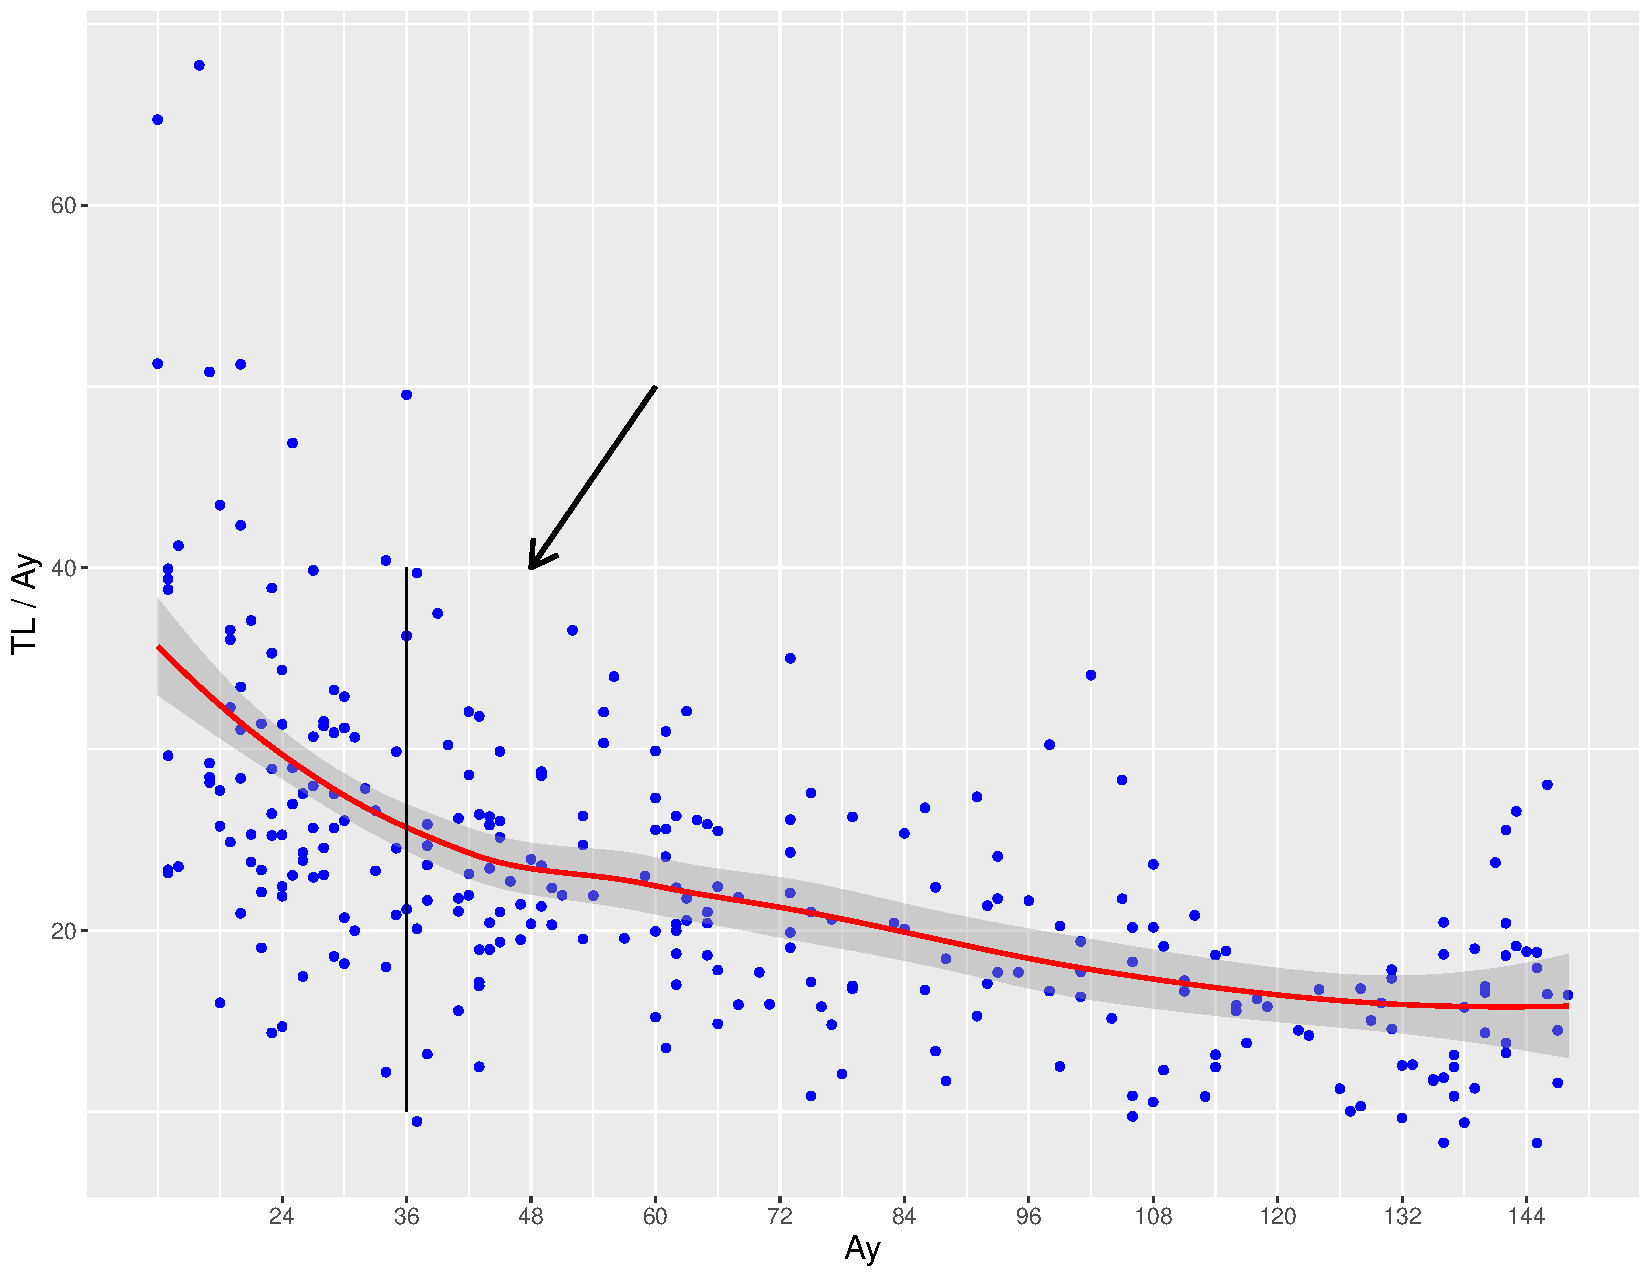
\includegraphics[width=1\linewidth, height=0.3\textheight]{../Figures/Fig1}
 	\end{center}
 	  %\vspace{0pt}
 	  \captionof{figure}{Aylara göre masraf kümelenmesi (TL/Ay)}
 	  \label{fig:Fig1}	
\end{minipage}
\begin{minipage}{0.49\textwidth}
	\begin{center}
	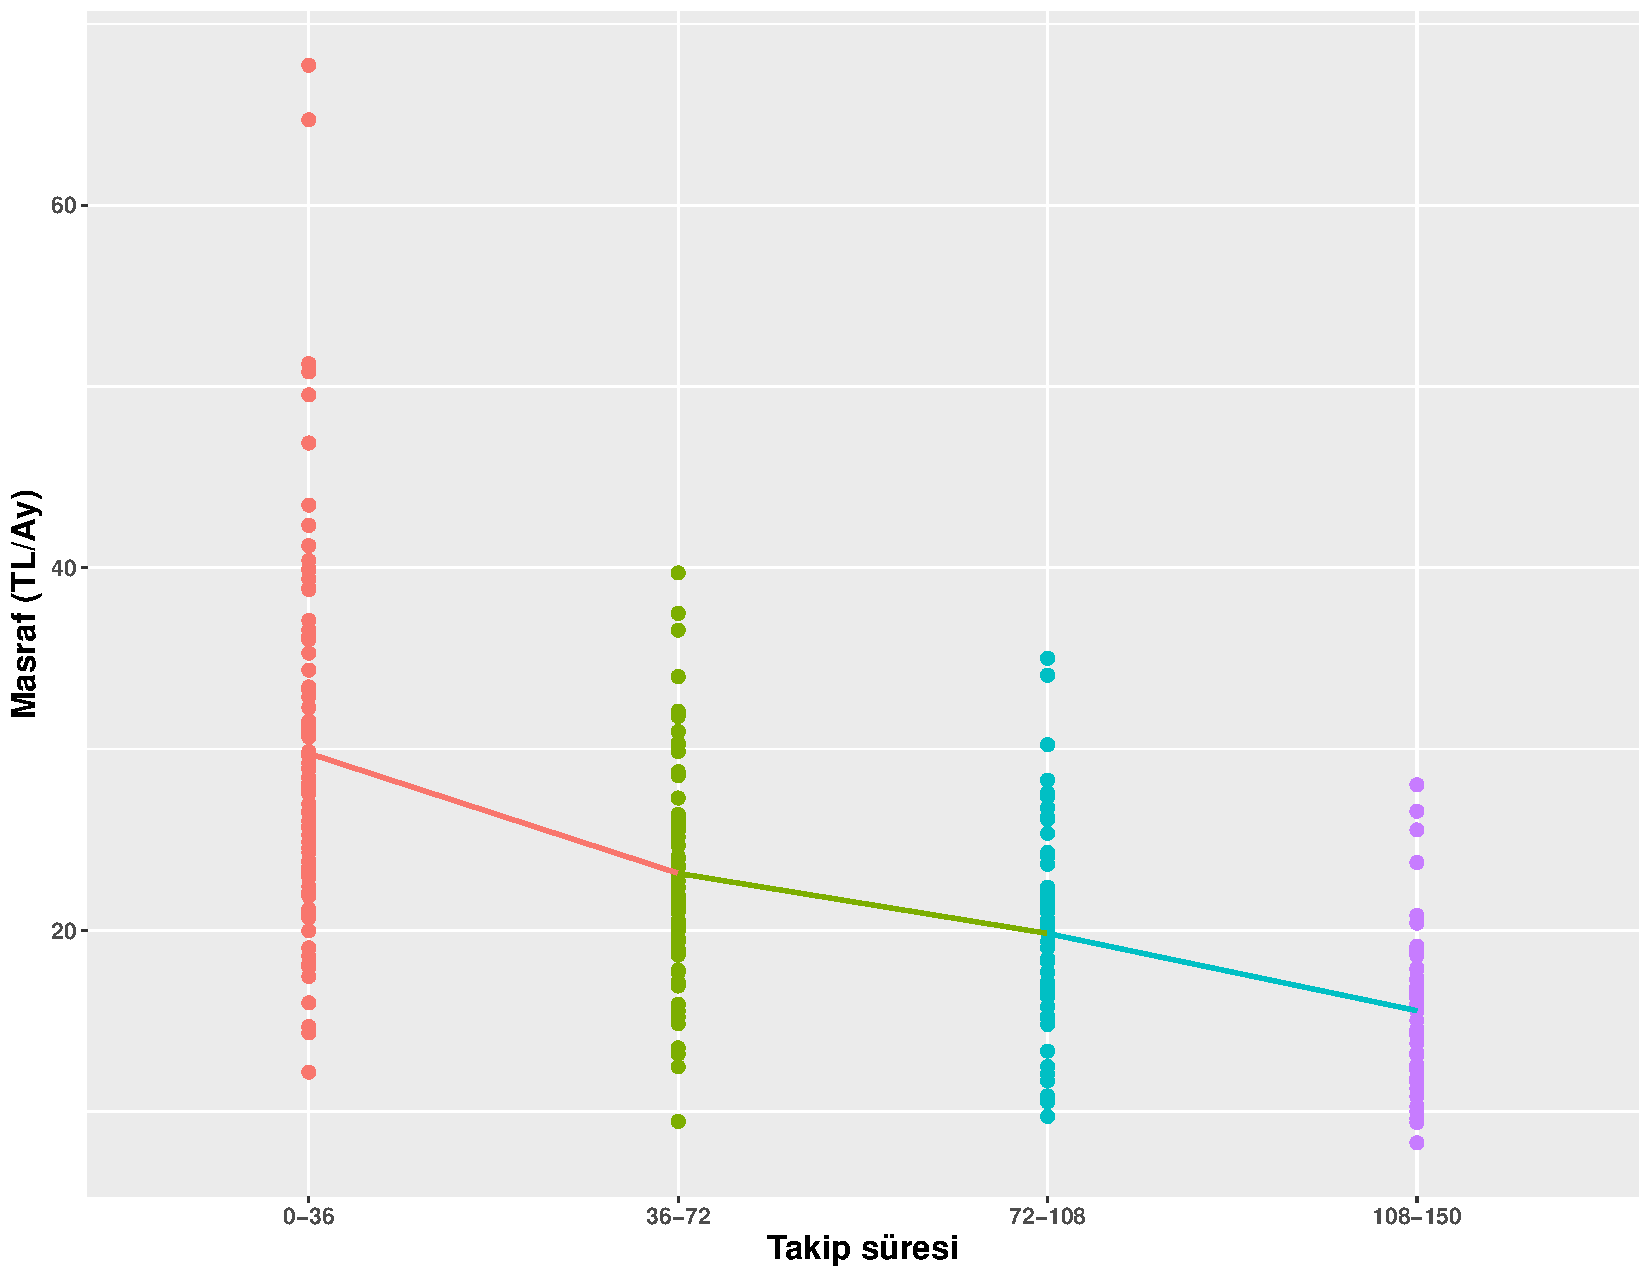
\includegraphics[width=1\linewidth, height=0.3\textheight]{../Figures/Fig2}
	\end{center}
	  %\vspace{0pt}
	  \captionof{figure}{Takip sürelerine göre masraf (TL/Ay)}
	  \label{fig:Fig2}
\end{minipage}\\  
  
  
  
Takip süresine göre testlerin hasta başına maliyeti Tablo \ref{tablo:tlhasta}'de gösterilmiştir. Oran olarak en çok masrafı HBV DNA oluşturmaktadır (Şekil \ref{fig:Fig5}). HBV DNA çıkartıldığında sırasıyla KC biyopsisi, AFP, üst batın USG ve HBsAg masrafı üstlenmektedir (Şekil \ref{fig:Fig6}) 
   
  
  \begin{longtable}{lcccc}\caption{Takip süresine göre testlerin hasta başına maliyeti} \label{tablo:tlhasta}\\
        \hline
          & 0-36 Ay & 36-72 Ay & 72-108 Ay & 108-150 Ay \\ 
    
       
        \hline
        \endfirsthead
        \multicolumn{5}{l}{\tablename\ \thetable{} \textit{-- önceki sayfadan devam ediyor}}\\
        \hline
          & 0-36 & 36-72 & 72-108 & 108-150 \\ 
        \hline
       
        \endhead
        \hline
        \multicolumn{5}{l}{\textit{devam ediyor}} \\
        \endfoot
        \multicolumn{3}{l}{}  \\
        \endlastfoot
  Hemogram & 12.03 & 22.34 & 47.93 & 36.67 \\ 
  ALT & 4.89 & 9.07 & 24.24 & 16.92 \\ 
  AST & 4.34 & 7.69 & 20.69 & 14.34 \\ 
  Albumin & 2.02 & 3.12 & 6.58 & 4.86 \\ 
  PT-APTT-INR & 5.35 & 6.68 & 23.15 & 13.32 \\
  AFP & 21.45 & 36.65 & 75.59 & 54.10 \\
  Anti-HCV & 5.96 & 6.17 & 18.30 & 11.29 \\ 
  Anti-HIV & 3.39 & 3.51 & 8.90 & 6.85 \\ 
  Anti-HAV IgG & 5.57 & 6.37 & 5.31 & 6.97 \\
  Anti-HBc IgM & 0.29 & 0.71 & 0.70 & 0.83 \\ 
  Anti-HBc IgG & 2.64 & 2.83 & 3.91 & 2.82 \\   
  HBsAg & 20.72 & 36.41 & 57.75 & 53.08 \\ 
  Anti-HBs & 9.88 & 17.40 & 33.66 & 24.91 \\ 
  HBeAg & 16.68 & 21.24 & 36.93 & 35.80 \\ 
  Anti-HBe & 17.21 & 21.34 & 34.22 & 36.53 \\ 
  HBV DNA & 469.85 & 828.10 & 1433.00 & 1207.35 \\ 
  Delta Antikoru & 14.75 & 20.74 & 27.90 & 26.82 \\ 
  Hepatobilier USG & 2.99 & 3.74 & 6.59 & 5.29 \\ 
  Tüm Batın USG & 20.36 & 39.72 & 34.91 & 35.57 \\ 
  Üst Batın USG & 18.70 & 36.56 & 69.72 & 59.06 \\ 
  Üst Batın MR & 8.34 & 28.35 & 25.54 & 36.42 \\ 
  KC biyopsisi & 23.33 & 34.48 & 57.14 & 79.25 \\
   \hline
                      \end{longtable}




\begin{minipage}{0.49\textwidth}
 \begin{center}
 	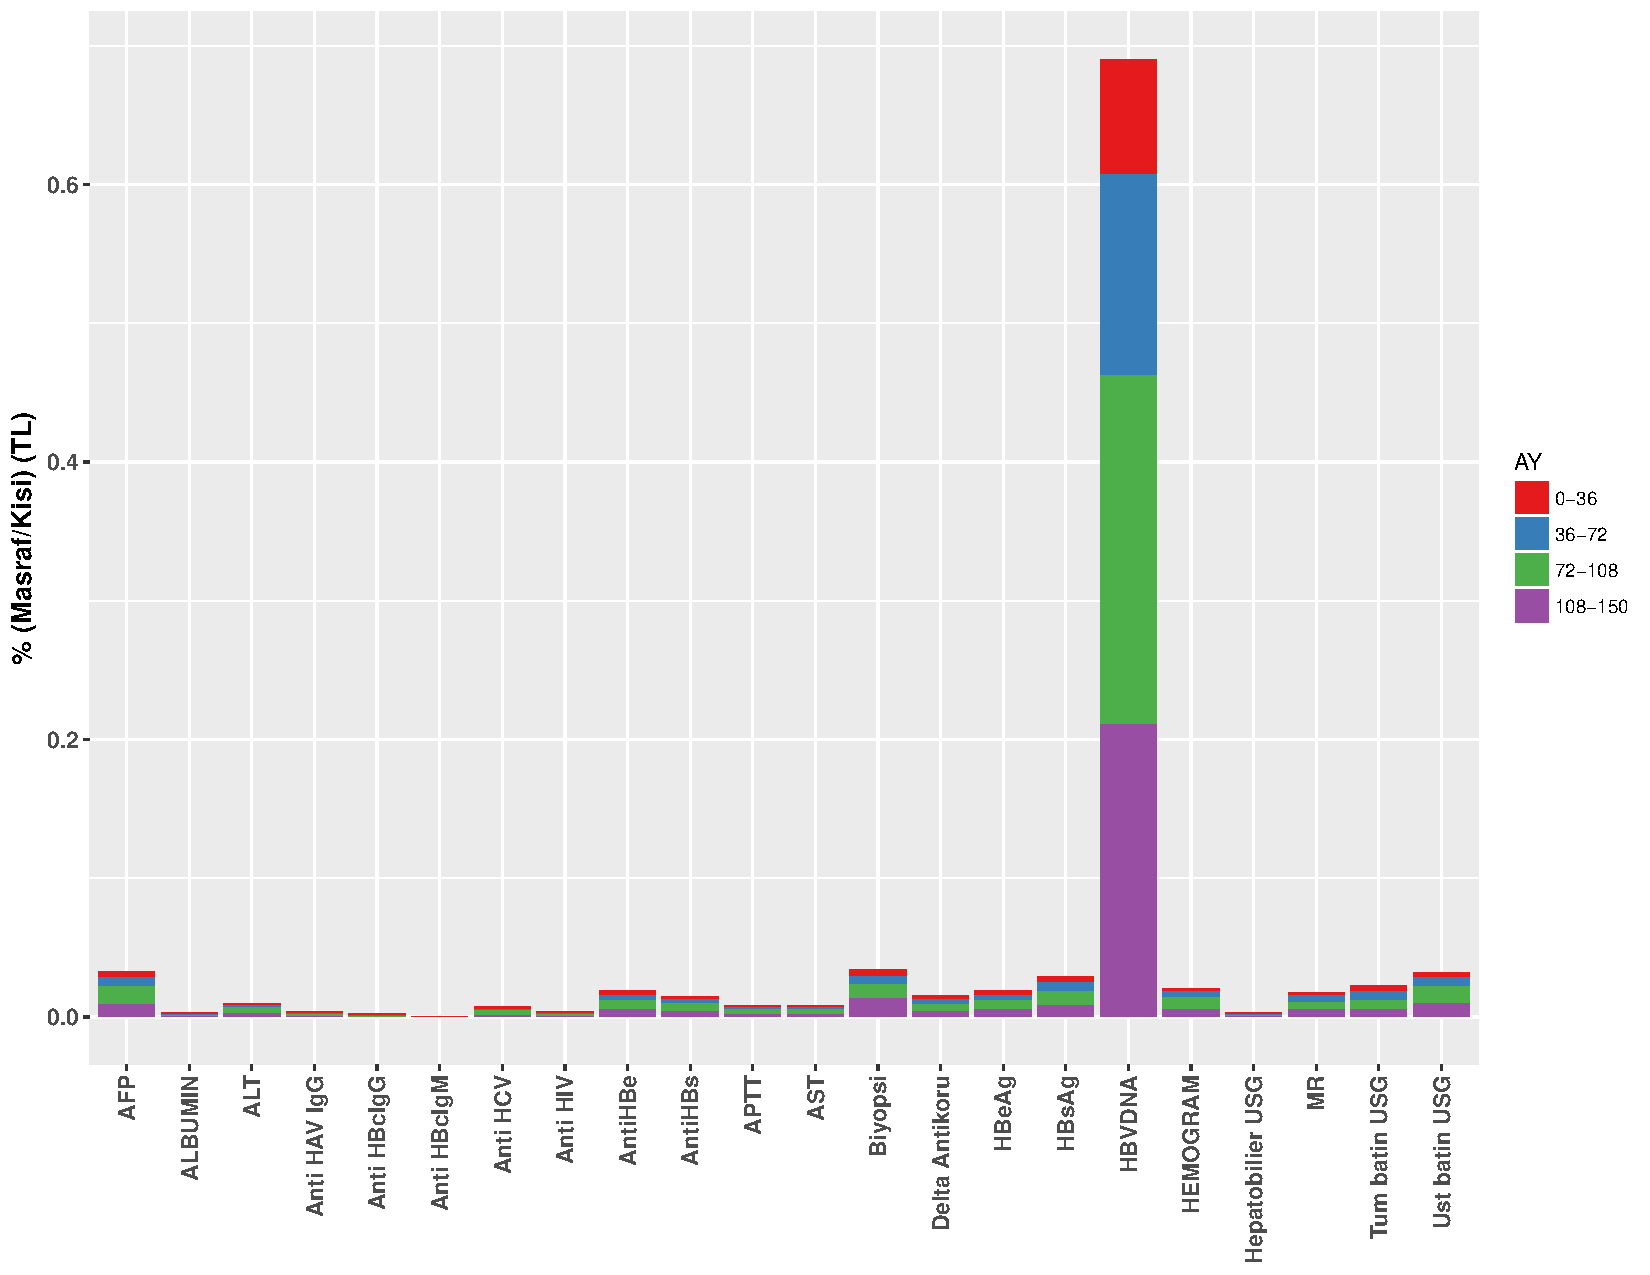
\includegraphics[width=1\linewidth, height=0.35\textheight]{../Figures/Fig5}
 	\end{center}
 	  %\vspace{0pt}
 	  \captionof{figure}{Takip süresine göre hasta başı maliyette testlerin yüzdeleri}
 	  \label{fig:Fig5}	
\end{minipage}
\begin{minipage}{0.49\textwidth}
	\begin{center}
	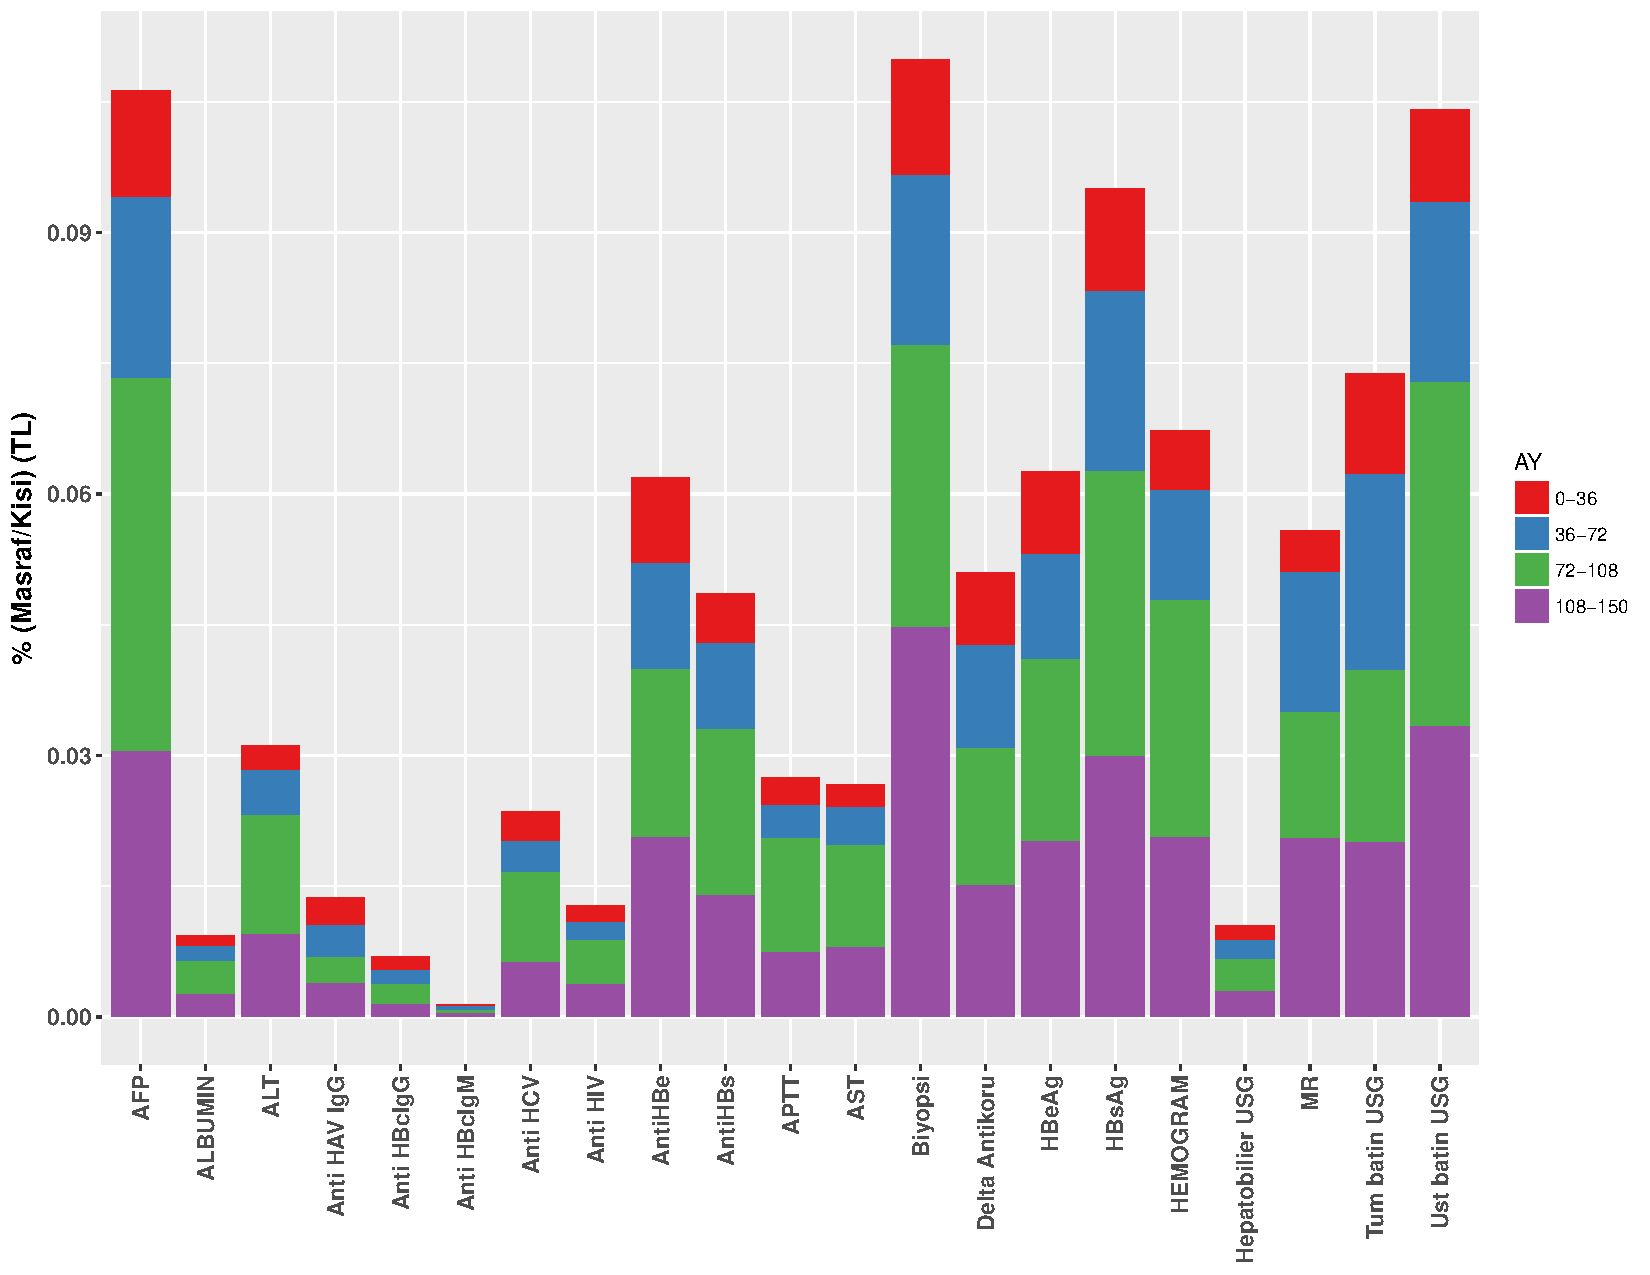
\includegraphics[width=1\linewidth, height=0.35\textheight]{../Figures/Fig6}
	\end{center}
	  %\vspace{0pt}
	  \captionof{figure}{Takip süresine göre hasta başı maliyette HBV DNA çıkartıldığında testlerin yüzdeleri}
	  \label{fig:Fig6}
\end{minipage}\\  










\phantomsection
	
	%----------------------------------------------------------------
\newpage
\chapter{TARTIŞMA ve SONUÇ} % Main chapter title
\label{STS} % For referencing the chapter elsewhere, use \ref{Chapter1} 
\lhead{\emph{Tartışma \& Sonuç}} % This is for the header on each page -
%perhaps a shortened title
%----------------------------------------------

% Tartışma

%-----------------------------------------------

\section{TARTIŞMA}

% % % % % % % % % % % % % % % % % % % % % % % % % % % % %

İnaktif taşıyıcı hastalar enfeksiyon hastalıkları polikliniğinde en fazla takip edilen hasta grubudur. Takibin amacı KHB'nin yol açabileceği komplikasyonları erken tanımaktır. Retrospektif çalışmamızda her yıl düzenli olarak kontrole gelen 293 hastanın ortalama 60 (30.0;102) ay takip süresi sonunda hiçbirisinde  siroz ya da hepatoselüler kanser gelişmemiştir. İnaktif taşıyıcılarda hastalığın doğal seyrinin incelendiği Avrupa kaynaklı retrospektif çalışmalara baktığımızda Magalhães'in çalışmasında \cite{magalhaes2015hepatitis} siroz ya da HCC gelişmemiş, Gigi ve ark. \cite{gigi2007long}'da ise bir siroz gelişmiş, hiç HCC gelişmemiştir. 

Prospektif çalışmalarda ise Avrupa kaynaklı kohortlarda da siroz ya da HCC bildirilmemiştir \cite{martinot2002serum,oliveri2017long,zacharakis2008role}. Tayvan kaynaklı çalışmalarda ise yüksek oranlar mevcuttur \cite{chen2010carriers,chu2007spontaneous,hsu2002long}. Bir Amerika kaynaklı çalışmada 2 hastada HCC saptanmıştır \cite{tong2013hepatitis}. Çalışmaların hasta sayısı, takip süresi ve komplikasyonların oranları Tablo \ref{tablo:lit}'de incelenebilir.

Çalışmamızda 18 (\%6) hastada HBsAg kaybı olmuştu. HBsAg kaybı oranı diğer Avrupa kaynaklı retrospektif çalışmalarla benzerdir (Magalhães'in çalışmasında \%4 \cite{magalhaes2015hepatitis}; Gigi ve ark \%7.8 \cite{gigi2007long}).  

Değinilen çalışmalar ışığında söylenebilir ki HBeAg negatif HBV enfeksiyonu doğru olarak tanımlandığında oldukça iyi seyirlidir. En sık senaryo hastaların herhangi bir komplikasyon gelişmeden yıllarca takibidir. İkinci senaryo spontan HBsAg kaybıdır. Siroz ve HCC oldukça nadirdir ve oranlar coğrafik farklılıklar göstermektedir. KHB için orta endemik olan ülkemizde KHB'nin en fazla hastayı içeren bu alt grubunun yıllarca takip edileceği düşünüldüğünde takibin periyodu ve hangi testlerle yapılacağı maliyet uygun yaklaşımları gerektirmektedir. Çalışmamızın amacı bu takip maliyetinin tanımlanmasıdır.

Çalışmamızda toplam en çok istenmiş ilk beş test sırasıyla ALT, AST, hemogram, HBV DNA ve AFP idi. Anlaşılmaktadır ki klasik ALT, HBV DNA yanında AST'yi ALT ile kombine değerlendirmekteyiz, hemogramı ise ya sirozun laboratuar bulgusu olarak sitopeni araştırmak (öz. trombositopeni) amaçlı ya da basit rutin olarak isteme yatkınlığımız bulunmakta. HCC taraması amacıyla da AFP'yi tercih etmekteyiz. 

Maliyet hesaplamalarında toplam en çok harcama yapılan test HBV DNA idi. İkinci sırada \%5.9 ile KC USG (hepatobilier USG, üst batın USG ve tüm batın USG toplandığında), sonrasında da sırasıyla KC biyopsisi (\%3,32) AFP (\%3.28) ve HBsAg (\%2.95) geliyordu. HBV DNA hasta başına toplam harcamanın \%69'unu oluşturuyordu.

37 hastaya toplam 43 defa yapılmış olmasına rağmen KC biyopsisi toplam masraflarda üçüncü sırada geliyordu. KC biyopsisi günübirlik yatış gerektirmesi, girişimsel radyoloji işlemi, işlem sonrası kontrol görüntüleme ve hemogram bakılması ve patolojik işlem girişi gerektirdiğinden en pahalı işlemdir. En çok KC biyopsisinin ALT normal, HBV DNA 2000 ile 20000 arası olan hastalara istenmiş olması ALT'den ziyade HBV DNA düzeyinin biyopsi kararımızı etkilediğini göstermiştir. Bunda geçmiş rehberlerin inaktif taşıyıcılıkta HBV DNA için 2000 IU/ml'yi eşik değer olarak belirlemesi rol oynamış olabilir.

Toplam masrafta olduğu gibi takip süresine göre vizit başına ve hasta başına da en çok masrafı HBV DNA oluşturuyordu. Takip süresine göre kategorilendirme yapıldığında (0-36 ay, 36-72 ay, 72-108 ay, 108-150 ay) vizit başına en çok masraf yapılan hastalar 0-36 ay aralığında takip edilmiş hastalardı. Takip süresi uzadıkça vizit başı maliyet düşerken 108-150 ay takip edilmiş hastalarda yeniden artıyordu. Bu durum yeni hastaların ilk başvuruda tüm tetkiklerinin yapılmasının ve ilk senelerde daha sık aralıklarla tetkik istenmesinin göstergesi olabilir. 

KHB'nin maliyetiyle ilgili daha çok aşılama maliyet etkinlik ve çeşitli tedavi stratejilerinin literatürdeki tedavi oranları eşliğinde simüle edildiği (Markov modellemesi) tedavi maliyet etkinlik çalışmaları yapılmıştır. Tedavisiz yıllarca takip edilen inaktif hastalarda maliyet tanımlama çalışmamızda literatürde benzer yayın bulmakta zorlandık. Ülkemizde yapılmış çalışmalara baktığımızda Karahasanoğlu ve ark.'ın 2013 yılında KHB ve kronik hepatit C'de takip, tedavi ve komplikasyonlarının maliyetinin araştırıldığı çalışmasında \cite{karahasanouglu2013costs} 158 inaktif taşıyıcının 1 yıllık takip sonrası maliyeti ortalama 178.10±161.74 Amerikan doları (dönemin dolar kuruyla çarptığımızda 320.58±291.132 TL) olarak hesaplanmıştır fakat yapılan testler ile ilgili detaylar belirtilmemiştir. Tosun'un 2007 yılında HBV ile savaşımda ülke kaynaklarının ekonomik kullanımı ile ilgili önerilerini sunduğu çalışmasında \cite{tosun2007hepatit} ilk kez HBsAg pozitifliği saptanan bir hastaya yapılması gereken ve yılda bir kez tekrarlanması önerilen tetkiklerin vizit başı maliyeti 199.80 TL, asemptomatik taşıyıcılara 3-6 ayda veya yılda bir kez yapılması gereken tetkiklerin vizit başı maliyeti ise 72 TL olarak hesaplanmıştır.

Tanımladığımız bulgular eşliğinde maliyet etkin takip için neler önerebiliriz? İnaktif taşıyıcılığın iyi seyrini dikkate alarak masrafın çoğunu üstlenen testlere odaklandığımızda takip periyodunun arttırılması (örn. altı ayda birden senede bire uzatılması) HBV DNA için maliyet uygun olabilir.  KC biyopsisi hem hasta için invaziv hem de en masraflı işlem olduğundan biyopsi kararının dikkatli verilmesi önemlidir. ALT hepatosit hasarını gösteren ucuz bir testtir, fiyatı HBV DNA'nın yüzde biridir. KHB'de dalgalı seyir gösterebilir. Antiviral verilmesine gerek olmayan HBeAg pozitif HBV enfeksiyonu (immuntoleran) ve HBeAg negatif HBV enfeksiyonunda (inaktif taşıyıcılık) sürekli normal ALT seyri vardır ve biyopside KC hasarı beklenmez ya da minimaldir. Dolayısıyla biyopsi kararında ALT yüksekliği durumunda şüphelenip HBV DNA ile ortak karara varmak gereksiz biyopsileri engelleyebilir. Bununla birlikte çoğu zaman farketmediğimiz bir ayrıntı olarak poliklinik ekranında gereksiz tetkik girişi yapmamaya özen gösterilmelidir. Örneğin siroz ve HCC için KC parenkim değerlendirmesi amaçlı USG istediğimizde "tüm batın USG" girişi yapıldığında ücretlendirme 26,18 TL; "hepatobilier USG" girişi yapıldığında ücretlendirme 11,22 TL olmaktadır. Tüm batın USG, hepatobilier USG'nin iki katından daha pahalıdır, aradaki fark aynı zamanda 12 tane ALT değerindedir.   





% % % % % % % % % % % % % % % % % % % % % % % % % % % % % %

\newpage

\section{TEZİN KISITLILIKLARI}


\begin{itemize}
\item KHB'ye bağlı siroz ya da HCC gelişmiş hastaların takibi gastroenteroloji polikliniğine kaymış olabileceğinden bu hastaların klinik seyri ve maliyeti değerlendirilememiştir.

\item Veri tabanına poliklinik başvuruları ve tetkikler toplam sayı olarak girildiğinden takip süresi boyunca istem seyrinin değerlendirmesi yapılamamıştır. 


\end{itemize}

  

% % % % % % % % % % % % % % % % % % % % % % % % % % % % % % %

% % % % % % % % % % % % % % % % % % % % % % % % % % % % % %

\newpage

\section{SONUÇ}

% % % % % % % % % % % % % % % % % % % % % % % % % % % % % %

\begin{itemize}

\item Çalışmamıza göre HBeAg negatif HBV enfeksiyonu takibinde toplam en çok istenmiş test ALT idi, sonrasında da sırasıyla AST, hemogram, HBV DNA ve AFP geliyordu.  Toplam, vizit başına ve hasta başına en fazla masraf HBV DNA'ya aitti. HBV DNA çıkarıldığında ise hasta başı en fazla masrafı sırasıyla KC biyopsisi, AFP, üst batın USG ve HBsAg oluşturuyordu.

\item 0-36 ay aralığında takip edilmiş hastaların diğer takip kategorilerine göre vizit başına maliyeti daha fazlaydı.

\item HBeAg negatif HBV enfeksiyonu doğru olarak tanımlandığında oldukça iyi seyirlidir. Orta endemik ülkemizde KHB'nin en çok hastayı içeren bu alt grubun kronik KC komplikasyonları açısından yıllarca takip edileceği düşünüldüğünde takipte maliyet uygun yaklaşımlar benimsenmelidir.

\item Takip periyodunun arttırılması, biyopsi yapılacak hastaya dikkatli karar verilmesi, özellikle görüntüleme tetkik girişlerinin uygun yapılması maliyeti düşürülebilir. 

\item Ülkemizde inaktif taşıcıların takip maliyetini tanımlayacak çalışmalar sağlık harcamalarında politika karar vericilerine yön gösterecektir.

\end{itemize}

  
\phantomsection
\cleardoublepage
	%-----------------------------------------------------------------
	% ÖRNEKLER görmek için uncomment yapınız
	% -----------------------------------------------------------------
	
	%	\newpage
\lhead{\emph{örnekler}}

Bkz referans \cite{jorgensen1979heparin}.
Tablo \ref{tablo:1}'de görüldüğü gibi;\footnote{dipnot eklemek için}

\begin{mycode}
	\begin{itemize}\itemsep-6pt 
	    	\item[\ding{51}] yes
		    \item[\ding{55}] no 
	\end{itemize}
\end{mycode}

\begin{itemize}\itemsep-6pt 
 \item[\ding{51}] yes
 \item[\ding{55}] no 
\end{itemize}


\begin{mycode}
	\begin{dingautolist}{192}\itemsep-6pt 
		 \item The first item
	\end{dingautolist}
\end{mycode}

\begin{dingautolist}{192}\itemsep-6pt 
\item The first item
\item The second item
\item The third item
\end{dingautolist}


\begin{mycode}
 \dingfill {228}
\end{mycode}

\dingfill {228}


\begin{enumerate}[1.]\itemsep-6pt
\item bir
\item iki
\item üç
\end{enumerate}

\begin{minipage}{0.45\textwidth}
	\begin{enumerate}[1.]\itemsep-6pt%for capital roman numbers.
		\item bir
		\item iki
		\item üç
	\end{enumerate}
\end{minipage}
\begin{minipage}{0.45\textwidth}
	\begin{enumerate}[a.]\itemsep-6pt
		\item bir
		\item iki
		\item üç
	\end{enumerate}
\end{minipage}\\[1cm]

\begin{figure}[tbph]
\centering
\includegraphics[width=3cm]{../Figures/263px-Kefir_glass_london_feb_10}
\caption[kfr]{Kefir bardağı}
\label{fig:263px-Kefir_glass_london_feb_10}
\end{figure}

Bu araya yazılarımızı yazabiliriz.

%\begin{landscape}
\begin{minipage}{\textwidth}
	\centering
	\begin{threeparttable}
		\caption{Tablo başlığı buraya yazılır}  \label{tablo:1} %Tablo başlığı ve referans etiketi
		% ---------------------------------------
		\begin{tabular}{lccccr}
			\hline\hline
			Ranks & FAVORABLE \tnote{*} &(\%) & UNFAVORABLE &(\%) & Total \\
			 \hline
			A& 23 & (91.4) & 7 & (8.6) & 81 \\ 
			B& 58 & (90.6) & 6 & (9.4) & 64 \\ 
			C& 10 & (25.6) & 29 & (74.4) & 39 \\
			\hline
		\end{tabular}
		%------------------------------------------	    
		\begin{tablenotes}
			\footnotesize
			\item[] buraya not ekle\\
			\item[*] the first note; %tabloya "\tnote{*}" ekleyin 
			\item[$\dag$] second note ; %tabloya "\tnote{$\dag$}" ekleyin
			%\item[$\ddag$] third note ;
			%\item[$\S$] third note ;
			%\item[**] the first note; 
		\end{tablenotes}
	\end{threeparttable}
\end{minipage}
%\end{landscape}



\pagebreak
%---------------------------------------------------------
% % % % % % % % % % % % % % % % % % % % % % % % % %
% % % % % % % % % % % % % % % % % % % % % % % % % % 
\begin{mycode}
 \begin{center}
\begin{threeparttable}
	\renewcommand{\arraystretch}{1.3}
	\rowcolors{2}{gray!20}{white}
	\caption{Üç parçalı tablo}
	\label{tablo:UP} %Tablo başlığı ve referans etiketi
	% -------------------------------------------------------
       \begin{tabular}{rccccc}
        	\hline\hline
        	Ranks & FAVORABLE \tnote{*} &(\%) & UNFAVORABLE &(\%) & Total \\ \hline
        	0 & 74 & (91.4) & 7 & (8.6) & 81 \\ 
        	1 & 58 & (90.6) & 6 & (9.4) & 64 \\ 
        	6 & 10 & (25.6) & 29 & (74.4) & 39 \\\hline
       \end{tabular}
	%-------------------------------------------------------	    
	\begin{tablenotes}
		\footnotesize
		\item[*] the first note; %tabloya "\tnote{*}" ekleyin 
		\item[$\dag$] second note ; %tabloya "\tnote{$\dag$}" ekleyin
		%\item[$\ddag$] third note ;
		%\item[$\S$] third note ;
		%\item[**] the first note; 
	\end{tablenotes}
\end{threeparttable}
 \end{center}
\end{mycode}


\begin{center}
\begin{threeparttable}
   \renewcommand{\arraystretch}{1.3}
   \rowcolors{2}{gray!20}{white}
    \caption{Üç parçalı tablo}
    \label{tablo:UP} %Tablo başlığı ve referans etiketi
% -------------------------------------------------------
       \begin{tabular}{rccccc}
	    \hline\hline
	    Ranks & FAVORABLE \tnote{*} &(\%) & UNFAVORABLE &(\%) & Total \\ \hline
	    0 & 74 & (91.4) & 7 & (8.6) & 81 \\ 
	    1 & 58 & (90.6) & 6 & (9.4) & 64 \\ 
	    6 & 10 & (25.6) & 29 & (74.4) & 39 \\\hline
	    \end{tabular}
%-------------------------------------------------------	    
\begin{tablenotes}
 \footnotesize
	\item[*] the first note; %tabloya "\tnote{*}" ekleyin 
	\item[$\dag$] second note ; %tabloya "\tnote{$\dag$}" ekleyin
	%\item[$\ddag$] third note ;
	%\item[$\S$] third note ;
	%\item[**] the first note; 
\end{tablenotes}
\end{threeparttable}
\end{center}

%-----------------------------------
%Örnek Tablo 1 (arraystrech ile satır büyüklüğü ayarlanır)
%----------------------------
\begin{table}[H]
\renewcommand{\arraystretch}{1.3}
\begin{tabular}{lclclclc}
\hline
\hline 
Month & Week & Programme \\
\hline
May & 3-4 & Cycle Tour \\
June & 1-2 & \textless DCP Project\\
July & 1-2 & \textgreater Clean Energy\\
August & 3-4 & Interim Report\\
\hline
\end{tabular}
\caption{Four months plan: where,what how}
\label{tab:tab1}
\end{table}
\newpage
Daha detaylı bilgi is tablo \ref{tab:tab2}'de görülüyor.
%------------------------------
%Örnek Tablo 2 burada L(left) R(right) J(center) ile genişlik ayarlanır Toplam size = column sayısıs
%-------------------------------
%--------------------------
%Tablo 3 profesyonel görünümlü tablo
%--------------------------
\begin{mycode}
  \begin{table}[H]
  	\renewcommand{\arraystretch}{1.3}
  	\begin{tabular}{l C{3cm} C{3cm}}
       	\toprule
            	& \mcc{Item}   \\
         \cmidrule(r){2-3}
            	Animal  & Description & Price \tablefootnote{der} (\$) \\ 
         \midrule
            	\mr{\rotatebox[origin=c]{90}{Gnat}} & per gram    & 13.65    \\
            	& each        & 0.01                           \\
            	Gnu \tablefootnote{man}             & stuffed     & 92.50  \\
            	Emu                                 & stuffed     & 33.33     \\
            	Armadillo                           & frozen      & 8.99  \\ 
          \bottomrule
  	\end{tabular}
  	\caption{Profes table}
  	\label{tab:tabP}
  \end{table}
\end{mycode}

\begin{table}[H]
\renewcommand{\arraystretch}{1.3}
\begin{tabular}{l C{3cm} C{3cm}}
	\toprule
	                                    & \mcc{Item}    \\
	\cmidrule(r){2-3}
          Animal  & Description & Price \tablefootnote{der} (\$) \\ \midrule
	\mr{\rotatebox[origin=c]{90}{Gnat}} & per gram    & 13.65                          \\
	                                    & each        & 0.01                           \\
	Gnu \tablefootnote{man}             & stuffed     & 92.50                          \\
	Emu                                 & stuffed     & 33.33                          \\
	Armadillo                           & frozen      & 8.99                           \\ \bottomrule
\end{tabular}
\caption{Profes table}
\label{tab:tabP}
\end{table}
%--------------------------
%Öbek Tablo 4
%--------------------------
% Table generated by Excel2LaTeX from sheet 'Sheet1'
\begin{table}[htpn]

  \centering
  \renewcommand{\arraystretch}{1.5}
  \caption{Add caption}
    \begin{tabular}{lC{3cm}r}
    	\toprule
    	değişken & ölen   & kalan \tablefootnote{ss} \\ \midrule
    	a        & $22^2$ &           $\leqslant$ 33 \\
    	b        & $3_2$  &           $\geqslant$ 66 \\ \bottomrule
    \end{tabular}%   
  \label{tab:tab4}%
\end{table}

\newpage
\begin{table}[c]
\hbox{
\rotcaption{Minimum number of individuals; effect of rotating table
and caption separately}\label{rotfloat3}%
\begin{sideways}
\begin{tabular}[t]{cccccccccR{3cm}}
\hline
Phase&Total&Cattle&Sheep&Pig&Red \tablefootnote{ilk kez} Deer&Horse&Dog&Goat&Other\\
\hline
&1121&54&12&32&1&1&1&1&1 polecat\\
3&8255&58&6&35&1&1&1&1&1 roe deer, 1 hare, 1 cat, 1 otter\\
4&543&45&6&45&4&1&1&---&---\\
\hline
&9919&157&24&112&6&3&3&2&5\\
\hline
\end{tabular}
\end{sideways}
}
\end{table}
\cleardoublepage

%--------------------------
%Burada resmi kestik ve çevirdik 
%---------------------------
\newpage
\pagestyle{fancy}
\begin{figure}[htpn]
\centering
\includegraphics[trim=2cm 2cm 1cm 1cm, clip=true, totalheight=0.2\textheight, angle=45]{../Figures/Electron}
\caption[elect2]{Electron grafiği}
\label{fig:Electr}
\end{figure}
%-------------------------------
% landscape page
%-------------------------------
\newpage
\pagestyle{plain}
\begin{landscape}
 % Table generated by Excel2LaTeX from sheet 'Sheet1'
 \begin{table}[htbp]
   \centering
   \caption{Add caption}
     \begin{tabular}{lccr}
     	\toprule
     	variables                                     &     FAVORABLE     & UNFAVORABLE \tablefootnote{dfıjreıo} &  \\
     	                                              &      (n=342)      &               (n=165)                &              p-value \\ \midrule
     	\multicolumn{1}{c}{}                          &                   &                                      & \multicolumn{1}{c}{} \\
     	Age (years), median (IQR)                     & 34.0 (23.0, 46.0) &          44.0 (28.0, 62.0)           &               <0.001 \\
     	Female gender                                 &   165 (48.2\%)    &             76 (46.1\%)              &                 0.64 \\
     	Elapsed time (days), median (IQR)             & 20.0 (10.0, 30.0) &          20.0 (12.0, 34.0)           &                 0.32 \\
     	AC / NV                                       &                   &                                      &               <0.001 \\
     	None                                          &    65 (19.0\%)    &              14 (8.5\%)              &  \\
     	Noisea vomiting \tablefootnote{bulantı kusma} &    89 (26.0\%)    &              11 (6.7\%)              &  \\
     	Altered consciousness                         &    67 (19.6\%)    &             80 (48.5\%)              &  \\
     	AC plus NV                                    &   121 (35.4\%)    &             60 (36.4\%)              &  \\
     	Altered consciousness                         &   188 (55.0\%)    &             140 (84.8\%)             &               <0.001 \\
     	Nausea/Vomiting                               &   210 (61.4\%)    &             71 (43.0\%)              &               <0.001 \\
     	Meningeal irritation sign                     &   231 (67.5\%)    &             121 (73.3\%)             &                 0.18 \\
     	Focal Neurological deficit                    &                   &                                      &               <0.001 \\
     	None                                          &   271 (79.2\%)    &             105 (63.6\%)             &  \\
     	Central\_Nerve\_Palsy                         &    38 (11.1\%)    &             24 (14.5\%)              &  \\
     	CNP plus MD                                   &     8 (2.3\%)     &              11 (6.7\%)              &  \\
     	Motor\_Deficit                                &    25 (7.3\%)     &             25 (15.2\%)              &  \\
     	Neurological deficit                          &    71 (20.8\%)    &             60 (36.4\%)              &               <0.001 \\
     	Central Nerve Palsy                           &    46 (13.5\%)    &             35 (21.2\%)              &                0.025 \\
     	2th Cranial Nerve                             &    21 (6.1\%)     &              6 (3.6\%)               &                 0.24 \\
     	3th Cranial Nerve                             &    16 (4.7\%)     &              12 (7.3\%)              &                 0.23 \\
     	Sequel                                        &     0 (0.0\%)     &             79 (47.9\%)              &  \\ \bottomrule
     \end{tabular}%
   \label{tab:addlabel}%
 \end{table}%
\end{landscape}
\newpage
\pagestyle{plain}
\begin{landscape}
\begin{figure}[htpn]
\centering
\includegraphics[width=0.3\linewidth]{../Figures/Electron}
\caption[e1]{Electron grafiği}
\label{fig:Electron}
\end{figure}
\end{landscape}
%---------------------------------
%Yazı resim etrafında
%---------------------------------
\newpage


\pagestyle{fancy}

\begin{mycode}
\begin{wrapfigure}[15]{l}[75pt]{10cm}
	\begin{center}
        	\includegraphics[width=0.5\linewidth, height=0.3\textheight]{../Figures/symbols}
        	\end{center}
        	\vspace{10pt}
        	\caption{\LaTeX \; için kullanılan semboller}
        	\label{fig:sym5}
\end{wrapfigure}
\end{mycode}


\begin{wrapfigure}[15]{l}[75pt]{10cm}
 \begin{center}
\includegraphics[width=0.5\linewidth, height=0.3\textheight]{../Figures/symbols}
\end{center}
  \vspace{10pt}
  \caption{\LaTeX \; için kullanılan semboller}
  \label{fig:sym5}
\end{wrapfigure}
Most gulls, particularly Larus species, are ground nesting carnivores, which will take live food or scavenge opportunistically. The live food often includes crabs and small fish. Apart from the kittiwakes, gulls  are typically coastal or inland species, rarely venturing far out to sea. The large species take up to four years to attain full adult plumage, but two years is typical for small gulls.
Gulls — the larger species in particular — are resourceful and highly-intelligent birds, demonstrating complex methods of communication and a highly-developed social structure. Certain species (e.g. the Herring Gull) have exhibited tool use behaviour. Many species of gull 
have learned to co-exist successfully with man and have thrived in human habitats. Others rely on kleptoparasitism to get their food.
%-------------------
% bölümleri ayırmak için
%-------------------
\phantomsection

\newpage

\begin{mycode}
\pagestyle{plain}
\topcaption{top caption}
  \tabletail{\hline \multicolumn{2}{r}{{Devam ediyor}} \\ }
  \tablehead{\hline variables & FAVORABLE & UNFAVORABLE&                        \\
	   &      (n=342)        &          (n=165)          &    \textit p-value \\ \hline }
         \begin{mpxtabular}{lccr}
        	Age (years), median (IQR)                & 34.0 (23.0, 46.0) & 44.0 (28.0, 62.0) & <0.001 \\
        	Female gender                            &   165 (48.2\%)    &    76 (46.1\%)    &   0.64 \\
        	Elapsed time (days), median (IQR)        & 20.0 (10.0, 30.0) & 20.0 (12.0, 34.0) &   0.32 \\
        	AC / NV                                  &                   &                   & <0.001 \\
        	Sequel                                   &     0 (0.0\%)     &    79 (47.9\%)    &  \\ 
        \bottomrule
         \end{mpxtabular}\\[3cm]
\cleardoublepage
\end{mycode}

\begin{center}
%\taburowcolors[2] 2{white .. lightgray}
\begin{longtabu} to \linewidth {X[3, l] X[2, l] X[2, c]}
\caption{Kohortun genel özellikleri} \label{tablo:TAB1}\\
 \toprule[1mm]
\textbf{FAKTÖRLER} &  & \textbf{DEĞER} \\
                   &  &  n(\%)\\
\hline
\endfirsthead
\textbf{FAKTÖRLER} &  & \textbf{DEĞER} \\
\hline
\endhead
\hline \multicolumn{3}{r}{\textit{Devam ediyor}} \\
\endfoot
\hline
\endlastfoot

                         	Yaş, ortalama (SS) &                            & 38.4 (11.9)       \\
\rowcolor{white!90!black}	Cinsiyet           & Erkek                      & 1188 (85.9)        \\


\end{longtabu}
\end{center}


\pagestyle{plain}
 \topcaption{top caption}
 \tabletail{\hline \multicolumn{2}{r}{{Devam ediyor}} \\ }
 \tablehead{\hline variables & FAVORABLE & UNFAVORABLE&                        \\
                                           &      (n=342)        &          (n=165)          &    \textit p-value \\ \hline }
 \begin{mpxtabular}{lccr}
 	Age (years), median (IQR)                & 34.0 (23.0, 46.0) & 44.0 (28.0, 62.0) & <0.001 \\
 	Female gender                            &   165 (48.2\%)    &    76 (46.1\%)    &   0.64 \\
 	Elapsed time (days), median (IQR)        & 20.0 (10.0, 30.0) & 20.0 (12.0, 34.0) &   0.32 \\
 	AC / NV                                  &                   &                   & <0.001 \\
 	None                                     &    65 (19.0\%)    &    14 (8.5\%)     &  \\
 	Noisea vomiting                          &    89 (26.0\%)    &    11 (6.7\%)     &  \\
 	Altered consciousness                    &    67 (19.6\%)    &    80 (48.5\%)    &  \\
 	AC plus NV                               &   121 (35.4\%)    &    60 (36.4\%)    &  \\
 	Altered consciousness                    &   188 (55.0\%)    &   140 (84.8\%)    & <0.001 \\
 	Nausea/Vomiting            L{4cm}l              &   210 (61.4\%)    &    71 (43.0\%)    & <0.001 \\
 	Meningeal irritation sign                &   231 (67.5\%)    &   121 (73.3\%)    &   0.18 \\
 	Focal Neurological deficit               &                   &                   & <0.001 \\
 	None                                     &   271 (79.2\%)    &   105 (63.6\%)    &  \\
 	Central\_Nerve\_Palsy                    &    38 (11.1\%)    &    24 (14.5\%)    &  \\
 	CNP plus MD                              &     8 (2.3\%)     &    11 (6.7\%)     &  \\
 	Motor\_Deficit                           &    25 (7.3\%)     &    25 (15.2\%)    &  \\
 	Neurological deficit                     &    71 (20.8\%)    &    60 (36.4\%)    & <0.001 \\
 	Central Nerve Palsy                      &    46 (13.5\%)    &    35 (21.2\%)    &  0.025 \\
 	2th Cranial Nerve                        &    21 (6.1\%)     &     6 (3.6\%)     &   0.24 \\
 	3th Cranial Nerve                        &    16 (4.7\%)     &    12 (7.3\%)     &   0.23 \\
 	Noisea vomiting \footnote{bulantı kusma} &    89 (26.0\%)    &    11 (6.7\%)     &  \\
 	Altered consciousness                    &    67 (19.6\%)    &    80 (48.5\%)    &  \\
 	AC plus NV                               &   121 (35.4\%)    &    60 (36.4\%)    &  \\
 	Altered consciousness                    &   188 (55.0\%)    &   140 (84.8\%)    & <0.001 \\
 	Nausea/Vomiting                          &   210 (61.4\%)    &    71 (43.0\%)    & <0.001 \\
 	Meningeal irritation sign                &   231 (67.5\%)    &   121 (73.3\%)    &   0.18 \\
 	Focal Neurological deficit               &                   &                   & <0.001 \\
 	None                                     &   271 (79.2\%)    &   105 (63.6\%)    &  \\
 	Central\_Nerve\_Palsy                    &    38 (11.1\%)    &    24 (14.5\%)    &  \\
 	CNP plus MD                              &     8 (2.3\%)     &    11 (6.7\%)     &  \\
 	Motor\_Deficit                           &    25 (7.3\%)     &    25 (15.2\%)    &  \\
 	Neurological deficit                     &    71 (20.8\%)    &    60 (36.4\%)    & <0.001 \\
 	Central Nerve Palsy                      &    46 (13.5\%)    &    35 (21.2\%)    &  0.025 \\
 	2th Cranial Nerve                        &    21 (6.1\%)     &     6 (3.6\%)     &   0.24 \\
 	3th Cranial Nerve                        &    16 (4.7\%)     &    12 (7.3\%)     &   0.23 \\
 	AC plus NV                               &   121 (35.4\%)    &    60 (36.4\%)    &  \\
 	Altered consciousness                    &   188 (55.0\%)    &   140 (84.8\%)    & <0.001 \\
 	Nausea/Vomiting                          &   210 (61.4\%)    &    71 (43.0\%)    & <0.001 \\
 	Meningeal irritation sign                &   231 (67.5\%)    &   121 (73.3\%)    &   0.18 \\
 	Focal Neurological deficit               &                   &                   & <0.001 \\
 	None                                     &   271 (79.2\%)    &   105 (63.6\%)    &  \\
 	Central\_Nerve\_Palsy                    &    38 (11.1\%)    &    24 (14.5\%)    &  \\
 	CNP plus MD                              &     8 (2.3\%)     &    11 (6.7\%)     &  \\
 	Motor\_Deficit                           &    25 (7.3\%)     &    25 (15.2\%)    &  \\
 	Neurological deficit                     &    71 (20.8\%)    &    60 (36.4\%)    & <0.001 \\
 	Central Nerve Palsy                      &    46 (13.5\%)    &    35 (21.2\%)    &  0.025 \\
 	2th Cranial Nerve                        &    21 (6.1\%)     &     6 (3.6\%)     &   0.24 \\
 	3th Cranial Nerve                        &    16 (4.7\%)     &    12 (7.3\%)     &   0.23 \\
 	AC plus NV                               &   121 (35.4\%)    &    60 (36.4\%)    &  \\
 	Altered consciousness                    &   188 (55.0\%)    &   140 (84.8\%)    & <0.001 \\
 	Nausea/Vomiting                          &   210 (61.4\%)    &    71 (43.0\%)    & <0.001 \\
 	Meningeal irritation sign                &   231 (67.5\%)    &   121 (73.3\%)    &   0.18 \\
 	Focal Neurological deficit               &                   &                   & <0.001 \\
 	None                                     &   271 (79.2\%)    &   105 (63.6\%)    &  \\
 	Central\_Nerve\_Palsy                    &    38 (11.1\%)    &    24 (14.5\%)    &  \\
 	CNP plus MD                              &     8 (2.3\%)     &    11 (6.7\%)     &  \\
 	Motor\_Deficit                           &    25 (7.3\%)     &    25 (15.2\%)    &  \\
 	Neurological deficit                     &    71 (20.8\%)    &    60 (36.4\%)    & <0.001 \\
 	Central Nerve Palsy                      &    46 (13.5\%)    &    35 (21.2\%)    &  0.025 \\
 	2th Cranial Nerve                        &    21 (6.1\%)     &     6 (3.6\%)     &   0.24 \\
 	3th Cranial Nerve                        &    16 (4.7\%)     &    12 (7.3\%)     &   0.23 \\
 	Sequel                                   &     0 (0.0\%)     &    79 (47.9\%)    &  \\ \bottomrule
 \end{mpxtabular}\\[3cm]
     \cleardoublepage

\begin{landscape}
\begin{ThreePartTable}
	\begin{TableNotes}
		\item[*] Bulantı kusma\\
		\item[] Another note
	\end{TableNotes}
	\begin{longtable}{L{9cm} c}
		\caption{Tablo başlığı}\\
		\toprule
		Column 1 & Column 2 \\
		\midrule
		\endhead
		\cmidrule{2-2}
		\multicolumn{2}{r}{\textit{devam ediyor}}
		\endfoot
		\bottomrule
		\insertTableNotes\\
		\endlastfoot
		%----tablo------

		Age (years), median (IQR)                 &  <0.001  \\ 
		Female gender                             &    0.64  \\ 
		Elapsed time (days), median (IQR)         &    0.32  \\ 
		AC / NV                                   &  <0.001  \\ 
		None                                      &    \\ 
		Noisea vomiting         \tnote{*}                  &    \\ 
		Altered consciousness                     &    \\ 
	\end{longtable}
\end{ThreePartTable}
\end{landscape}



	%	\newpage
\lhead{\emph{örnekler}}

\tcbset{colframe=blue!50!black,colback=red!5!white,
	boxsep=0pt,top=1mm,bottom=1mm,left=1mm,right=1mm,
	nobeforeafter,width=(\linewidth-2mm)/3}
\tcboxfit[height=8cm]{\lipsum[1]}\hfill
\tcboxfit[height=4cm]{\lipsum[1]}\hfill
\tcboxfit[height=2cm]{\lipsum[1]}

\tcbset{before upper={\textit{The story:}\par},
	colback=red!5!white,colframe=red!75!black,fonttitle=\bfseries,width=(\linewidth)}
\begin{tcolorbox}[title=My title]
	This is a \textbf{tcolorbox}.
\end{tcolorbox}


\begin{enumerate}[1.]\itemsep-6pt
	\item bir
	\item iki
	\item üç
\end{enumerate}
-------------------------------------------

\begin{minipage}{0.45\textwidth}
	\begin{enumerate}[1.]\itemsep-6pt%for capital roman numbers.
		\item bir
		\item iki
		\item üç
	\end{enumerate}
\end{minipage}
\hfill
\begin{minipage}{0.45\textwidth}
	\begin{enumerate}[a.]\itemsep-6pt
		\item bir
		\item iki
		\item üç
	\end{enumerate}
\end{minipage}\\[3cm]
-----------------------------------------------------------------------------------
\newpage
\begin{figure}[tbph]
\centering
\includegraphics[width=3cm]{../Figures/263px-Kefir_glass_london_feb_10}
\caption[kfr]{Kefir bardağı}
\label{fig:263px-Kefir_glass_london_feb_10}
\end{figure}
-------------------------------------------------------------------------------------
\newpage
%\begin{landscape}
\begin{minipage}[c]{\textwidth}
	\renewcommand{\arraystretch}{1.3} % SATIR ARALIĞI BELİRLEMEK İÇİN SAYIYI DEĞİŞTİRİN
	\centering
	\begin{threeparttable}
		\caption{Tablo başlığı buraya yazılır}  \label{tablo:1} %Tablo başlığı ve referans etiketi
		% ---------------------------------------
		\begin{tabular}{lccccr}
			\hline\hline
			Ranks & FAVORABLE \tnote{*} &(\%) & UNFAVORABLE &(\%) & Total \\
			 \hline
			A& 23 & (91.4) & 7 & (8.6) & 81 \\ 
			B& 58 & (90.6) & 6 & (9.4) & 64 \\ 
			C& 10 & (25.6) & 29 & (74.4) & 39 \\
			\hline
		\end{tabular}
		%------------------------------------------	    
		\begin{tablenotes}
			\footnotesize
			\item[] buraya not ekle\\
			\item[*] the first note; %tabloya "\tnote{*}" ekleyin 
			\item[$\dag$] second note ; %tabloya "\tnote{$\dag$}" ekleyin
			%\item[$\ddag$] third note ;
			%\item[$\S$] third note ;
			%\item[**] the first note; 
		\end{tablenotes}
	\end{threeparttable}
\end{minipage}
%\end{landscape}


\pagebreak
Bu tablo bir sayfayı aşacak büyük tablolar için tercih edilebilir\\
SAYFA ENİ KULLANILACAK İSE  \% $ \backslash$newpage, \% $ \backslash$pagestyle{plain}, \% $ \backslash$begin\{landscape\}   ve \% $ \backslash$end\{landscape\} "\%" KALDIRILIR
% % % % % % % % % % % % % % % % % % % % % % % % % % % % % % %
% %TABLO ÖRNEĞİ
% % % % % % % % % % % % % % % % % % % % % % % % % % % % % % %
%\newpage
%\pagestyle{plain}
%\begin{landscape}  
	\begin{ThreePartTable}
		\renewcommand{\arraystretch}{1} % SATIR ARALIĞI BELİRLEMEK İÇİN SAYIYI DEĞİŞTİRİN
%------------------NOTLAR
			\begin{TableNotes}
				\footnotesize
				\item[] Buraya tanımlar eklenebilir DDT, dedete; TBL, tablo; \dots  \\
				\item[*] Sakatlık veya ölüm; %tabloya "\tnote{*}" ekleyin 
				\item[$\dag$] Bulantı kusma ; %tabloya "\tnote{$\dag$}" ekleyin
				%\item[$\ddag$] third note ;
				%\item[$\S$] third note ;
				%\item[**] the first note; 
			\end{TableNotes}
%--------KOLON SAYISI -- BAŞLIK ve ETİKET  ---KOLON BAŞLIKLSRI
		\begin{longtable}{L{5cm}ccr} % KOLON SAYISI left (l) right(r) center(c) veya sabit genişlik için L{Xcm}R, {Xcm]}C{Xcm}
			
			\caption{Tablo başlığı} \label{tablo:2} \\ %BAŞLIK ve ETİKET
			\toprule\toprule
			Ranks & FAVORABLE & UNFAVORABLE \tnote{*}& \textit p-value \\ % KOLON BAŞLIKLARI
			\midrule
			\endhead
			\cmidrule{2-2}
			\multicolumn{2}{r}{\textit{devam ediyor}}
			\endfoot
			\bottomrule
			\insertTableNotes  \\
			\endlastfoot
% % % %---TABLO----------------------------------------------
			Age (years), median (IQR)                 & 5(22.3)& 8(30)&  <0.001  \\ 
			Female gender                             & & &    0.64  \\ 
			Elapsed time (days), median (IQR)         & & &    0.32  \\ 
			AC / NV                                   & & &  <0.001  \\ 
			None                                      & & &    \\ 
			Noisea vomiting   \tnote{$\dag$}        & & &    \\ 
			Altered consciousness                     & & &    \\ 	
% % % % %--tablo sonu------------------------------------------& 
		\end{longtable}
	\end{ThreePartTable}
%\end{landscape}
% % % % % % % % % % % % % % % % % % % % % % % % % % % % % % % % % % % % % % %
%TABLO SONU
% % % % % % % % % % % % % % % % % % % % % % % % % % % % % % % % % % % % % % % %
	%	\phantomsection
	%	\cleardoublepage
	
	%----------------------------------------------------------------------------------------
	%	BIBLIOGRAPHY
	%----------------------------------------------------------------------------------------
\phantomsection 
\label{Bibliography}
%\hyphenpenalty=1000000
\addtotoc{\bibname}
\setstretch{1.3}
\lhead{\emph{Kaynaklar}} % Change the page header to say "Bibliography"
%\bibliographystyle{vancouver_jit} 
\bibliographystyle{vancouver2} %Journal italic
%\bibliographystyle{unsrtnat}
%\bibliographystyle{plainnat}
%\bibliographystyle{abbrvnat
\bibliography{Chapters/2.Bibliography}
	% % % % % % % % % % % % % % % % % % % % % % % % % % % % % % % % % % % % % % % %
	%% % % % % %
	
	%----------------------------------------------------------------------------------------
	%	EKLER
	----------------------------------------------------------------------------------------
	%	\phantomsection
	%	\appendix
	%----------------------------------------
\phantomsection
\clearpage
\addtotoc{Etik Kurul Onay Formu}
\lhead{EK A. \emph{Etik Kurul Onay Formu}} % This is for the header
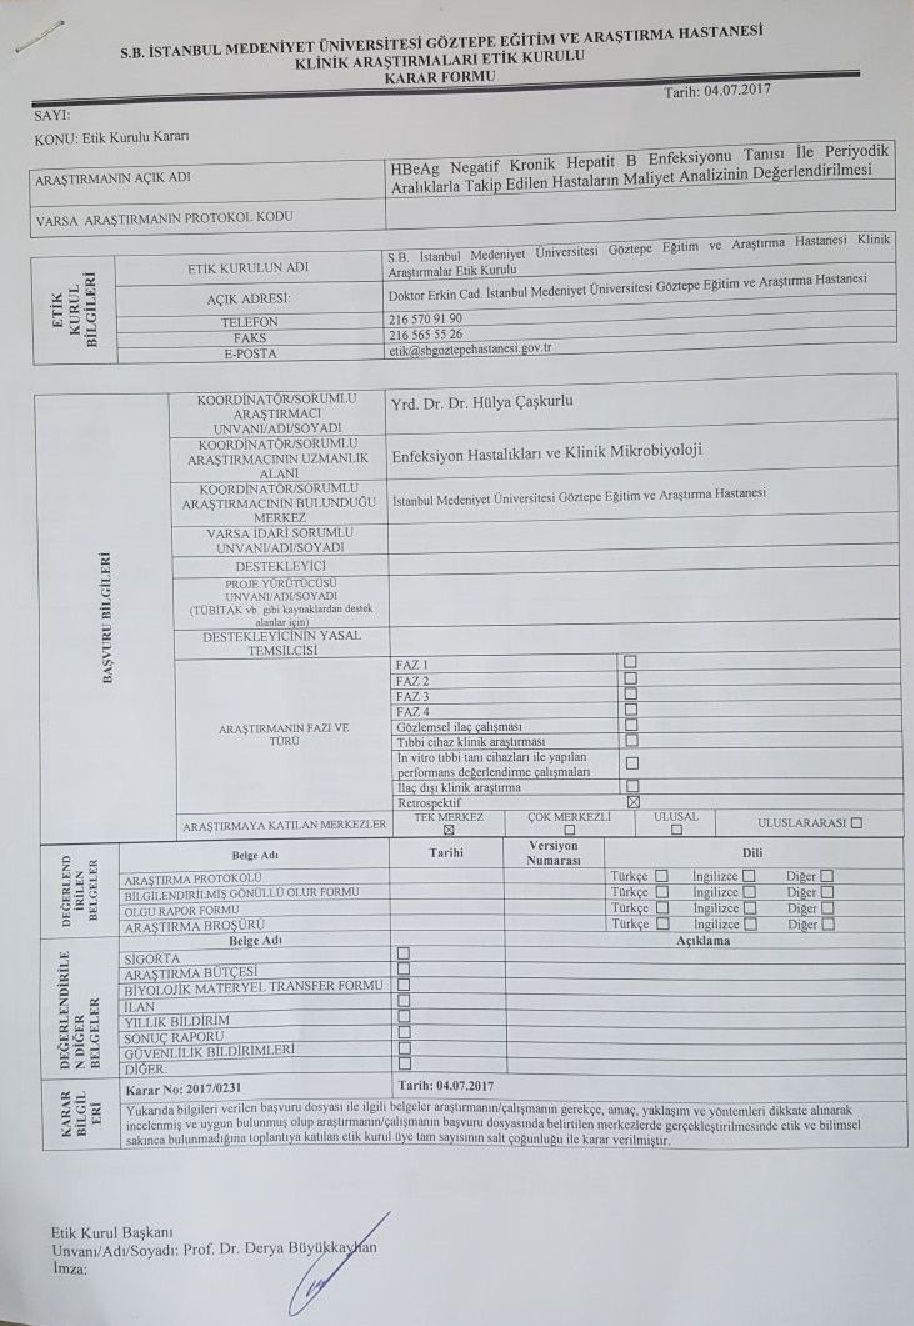
\includepdf[pages={1},offset=80 -50, scale=0.73, pagecommand={\thispagestyle{fancy}}] {onam.pdf} %onam formu "onam.pdf" olarak
%Figures altına yerleştirilecek
\phantomsection
\clearpage
%\addtotoc{Etik Kurul Onay Formu}
\lhead{EK A. \emph{Etik Kurul Onay Formu}} % This is for the header
\includepdf[pages={2},offset=80 -50, scale=0.73,
pagecommand={\thispagestyle{fancy}}] {onam.pdf} %onam formu "onam.pdf" olarak
%Figures altına yerleştirilecek
	%-------------------
	% bölümleri ayırmak için
	%-------------------
	\cleardoublepage
	\phantomsection
	\backmatter
	
	%--------------------------------------------------------------------------------------
	%TEZ DEĞERLENDİRME FORMU
	%--------------------------------------------------------
%\phantomsection
%\cleardoublepage
%\pagestyle{empty}
%



\renewcommand*{\LayoutTextField}[2]{\makebox[1em][l]{#1 }%
   \raisebox{\baselineskip}{\raisebox{-\height}{#2}}}

%\renewcommand{\LayoutChoiceField}[2]{%
%\makebox[2.5em][l]{#2}\parbox[t]{\linewidth}{#1}%
%}
%\changepage{}{20mm}{}{-10mm}{}{}{}{}{}
\newgeometry{left=5cm,top=4cm,bottom=2cm,right=0.1cm}

\begin{center}
T.C.\\
SAĞLIK BAKANLIĞI\\
İSTANBUL MEDENİYET ÜNİVERSİTESİ\\
GÖZTEPE EĞİTİM ve ARAŞTIRMA HASTANESİ\\[2mm]
{\small \textbf{TEZ DEĞERLENDİRME FORMU}}
\end{center}

\begin{Form}[action=mailto:imutipfakultesi@medeniyet.edu.tr,encoding=html,method=post]

\begin{tabular}{R{3cm}L{12cm}}
\textbf{TEZ BAŞLIĞI}: & {\footnotesize \ttitle} \\
\textbf{YAZAR}: & \authornames \\
\textbf{DANIŞMAN}: & \supname  \\
                   & %\supnameh\\    
\end{tabular}

%\begin{tabular}{R{3cm}L{12cm}}
%\textbf{TEZ BAŞLIĞI} & \TextField[name=tb,default=, multiline=true, height=1.2cm, width=11cm, charsize=10pt, bordercolor=0 1 1, borderwidth=0, backgroundcolor={.95 .95 .95}]{\mbox{}} \\[6mm]
%\textbf{YAZAR} & \TextField[name=y,default=, multiline=false, width=6cm,charsize=10pt, bordercolor=0 1 1,borderwidth=0,backgroundcolor={.95 .95 .95}]{\mbox{}} \\
%\textbf{DANIŞMAN} &  \TextField[name=d,default=, multiline=false, width=6cm,charsize=10pt, bordercolor=0 1 1,borderwidth=0,backgroundcolor={.95 .95 .95}]{\mbox{}}  \\
%\end{tabular}

\begin{tabbing}
\hspace*{10.2cm}\=\hspace*{1.5cm}\= \kill
\> \; VAR \> YOK \\[2mm]
SCI-Exp Kapsamında Yayınlanma Potansiyeli \> \ChoiceMenu[radio,radiosymbol=\ding{52}, name=yp,charsize=14pt, bordercolor=0 1 1,]{\mbox{}}{\mbox{},\mbox{\space\space\space\space}}\\[3mm]
Patent Alma Potansiyeli \> \ChoiceMenu[radio,radiosymbol=\ding{52}, name=pp,charsize=14pt, bordercolor=0 1 1,]{\mbox{}}{\mbox{},\mbox{\space\space\space\space}}\\[2mm]
\end{tabbing} 

\begin{tabbing}
\hspace{3.3 cm} \= \kill
KARAR \> \ChoiceMenu[combo,name=karar, width=8cm,charsize=10pt,bordercolor=0 1 1, default=]{\mbox{}}
{,BAŞARILI, DEĞİŞİKLİK YAPILMASI GEREKİR, BAŞARISIZ} \\[4mm]
YORUMLAR \> \TextField[name=Comment,default=, multiline=true,height=10\baselineskip,
  width=12cm,charsize=10pt, bordercolor=0 1 1,borderwidth=0,backgroundcolor={.95 .95 .95}]{\mbox{}} \\[4mm]
\end{tabbing}

%\begin{textblock}{3}(7.7,-0.2)
%...
%\end{textblock}

%\begin{textblock}{3}(8,-0.2)
%Tarih:
%\end{textblock}

\begin{tabbing}
\hspace*{10cm}\= \hspace*{3cm}\= \kill
\> Tarih \' \TextField[name=t,default= ... / ... / 20.., multiline=false, width=3cm,charsize=10pt, bordercolor=0 1 1,borderwidth=0,backgroundcolor={.95 .95 .95}]{\mbox{}}\\
\> İsim Soyad \' \TextField[name=isim,charsize=10pt, width=5.3cm,charsize=10pt, borderwidth=0,bordercolor=0 1 1,,backgroundcolor=0.95 0.95 0.95]{}\\[2mm]
\> İmza \'
\end{tabbing}

\vfill
\Reset[borderwidth=0,color=0.5 0.5 0.5]{Temizle} \quad \Submit[borderwidth=0]{Gönder} \quad  \Acrobatmenu{Print}{Yazdır}
\end{Form}

%\restoregeometry
	
	%\phantomsection
	%\cleardoublepage
	%\pagestyle{empty}
	%\renewcommand*{\LayoutTextField}[2]{\makebox[1em][l]{#1: }%
   \raisebox{\baselineskip}{\raisebox{-\height}{#2}}}

%\renewcommand{\LayoutChoiceField}[2]{%
%\makebox[2.5em][l]{#2}\parbox[t]{\linewidth}{#1}%
%}
%\changepage{}{20mm}{}{-10mm}{}{}{}{}{}
\newgeometry{left=5cm,top=4cm,bottom=0.1cm,right=0.1cm}

\begin{center}
T.C.\\
SAĞLIK BAKANLIĞI\\
İSTANBUL MEDENİYET ÜNİVERSİTESİ\\
GÖZTEPE EĞİTİM ve ARAŞTIRMA HASTANESİ\\[2mm]
{\small \textbf{TEZ DEĞERLENDİRME FORMU}}
\end{center}

\begin{Form}[action=mailto:imutipfakultesi@medeniyet.edu.tr,encoding=html,method=post]

\begin{tabular}{R{5cm}L{11cm}}
\textbf{ADI SOYADI}: & \authornames \\
\textbf{GÖREVİ}: &  {\footnotesize \MakeUppercase{\klinikname}} \\
\textbf{ADAYIN HAZIRLIDIĞI TEZİN ADI}: &  {\footnotesize \ttitle} \\[4mm]
\end{tabular}
\bigskip



{\small \begin{tabbing}
\hspace*{9cm}\=\hspace*{1.2cm}\= \kill
1. SAYFA SAYISI : \> \TextField[name=sayfa, charsize=9pt, width=2cm,bordercolor=0 1 1, borderwidth=0, backgroundcolor={.9 .9 .9}]{\mbox{}}\\[2mm]
2. TABLO SAYISI : \> \TextField[name=tablo, width=2cm,charsize=9pt,bordercolor=0 1 1, borderwidth=0, backgroundcolor={.9 .9 .9}]{\mbox{}}\\[2mm]
3. ŞEKİL : \> \TextField[name=sekil, width=2cm,charsize=9pt,bordercolor=0 1 1, borderwidth=0, backgroundcolor={.9 .9 .9}]{\mbox{}}\\[2mm]
4. İSTATİSTİK SAYISI : \> \TextField[name=ist, charsize=9pt, width=2cm,bordercolor=0 1 1, borderwidth=0, backgroundcolor={.9 .9 .9}]{\mbox{}}\\[2mm]
5- LİTERATÜR SAYISI VE FAYDALANMA DURUMU : \> \TextField[name=lit, width=7cm,bordercolor=0 1 1, borderwidth=0, charsize=9pt,backgroundcolor={.9 .9 .9}]{\mbox{}}\\[2mm]
6-YAZI TERTİBİ : \> \TextField[name=yazitertibi, charsize=9pt,width=7cm,bordercolor=0 1 1, borderwidth=0, backgroundcolor={.9 .9 .9}]{\mbox{}}\\[2mm]
7- KONUYU ANLATMA VE KONUYA HAKİMİYETI : \> \TextField[name=konu,charsize=9pt, width=7cm,bordercolor=0 1 1, borderwidth=0, backgroundcolor={.9 .9 .9}]{\mbox{}}\\[2mm]
8- İNCELEMENİN BİLİMSEL BAKIMDAN TUTUMU : \> \TextField[name=bilimsellik,charsize=9pt, width=7cm,bordercolor=0 1 1, borderwidth=0, backgroundcolor={.9 .9 .9}]{\mbox{}}\\[2mm]
9- ORİJİNAL OLUP OLMADIĞI :\> \TextField[name=bilimsellik,charsize=9pt, width=7cm,bordercolor=0 1 1, borderwidth=0, backgroundcolor={.9 .9 .9}]{\mbox{}}\\[2mm]
\end{tabbing}}



\begin{tabbing}
\hspace*{5cm}\= \hspace*{3cm}\= \hspace*{7cm}\= \kill
\> \textbf{SONUÇ} \> \ChoiceMenu[combo,name=karar,width=8cm,charsize=12pt,bordercolor=0 1 1, default=BAŞARILI]{\mbox{}}{BAŞARILI, DEĞİŞİKLİK YAPILMASI GEREKİR, BAŞARISIZ} \\[2mm]
\end{tabbing}






\begin{textblock}{3}(8.5,.5)
\hfill \today\\
\end{textblock}

\vspace*{2cm}
\begin{tabbing}
\hspace*{7cm}\= \hspace*{3cm}\= \kill
\> İsim Soyad \> \TextField[name=isim,charsize=10pt, width=5cm,borderwidth=0,bordercolor=0 1 1,,backgroundcolor=0.9 0.9 0.9]{}\\
\> İmza:
\end{tabbing}



\vfill
\Reset[borderwidth=0,color=0.5 0.5 0.5]{Temizle} \quad \Submit[borderwidth=0]{Gönder} \quad  \Acrobatmenu{Print}{Yazdır}
\end{Form}


	
	
\end{document}
